\documentclass[12pt,MSc,wordcount,twoside,anon]{muthesis}
% The regulations say that 12pt should be used
% Change the MSc option to MPhil, MRes or PhD if appropriate

\usepackage{verbatim}
\usepackage{graphicx}
\usepackage{url} % typeset URL's reasonably
\usepackage{listings}
\usepackage{float}
\usepackage{amsfonts}
\usepackage{algorithm}
\usepackage{algpseudocode}
\usepackage{mathtools}
\usepackage{hyperref}
\newcommand{\tabincell}[2]{\begin{tabular}{@{}#1@{}}#2\end{tabular}}
\hypersetup{
    colorlinks=true,
    linkcolor=black,
    urlcolor=blue,
    linktoc=all,
    citecolor=black
}
% \usepackage[numbers]{natbib}
% \usepackage{apacite}

\usepackage{pslatex} % Use Postscript fonts

% Uncomment the next line if you want subsubsections to be numbered
%\setcounter{secnumdepth}{3}
% Uncomment the next line if you want subsubsections to be appear in
% the table of contents
%\setcounter{tocdepth}{3}

% Uncomment the following lines if you want to include the date as a
% header in draft versions
%\usepackage{fancyhdr}
%\pagestyle{fancy}
%\lhead{}  % left head
%\chead{Draft: \today} % centre head
%\lfoot{}
%\cfoot{\thepage}
%\rfoot{}

\begin{document}
% Uncomment the following lines to leave out list of figures, tables
% and copyright until final printing
%\figurespagefalse
%\tablespagefalse
%\copyrightfalse
% \raggedright

\title{AI-powered CV Checker}
\author{Xinyi OUYANG}
\stuid{10861766}
\principaladviser{Ducan Hull}

\beforeabstract

\prefacesection{Abstract}
\abstracttitle
% Single spacing can be turned on for the abstract
%
{\singlespacing

In recent years, e-recruitment systems have been augmented, and the mode of uploading resumes online to apply for positions has been popularized. In this situation, checking the resume automatically can fit the e-recruitment mode and help job seekers modify their CVs to match the target position better. There have been several powerful CV checkers such as CareerSet, which can provide comprehensive feedback on the resume. However, the inside techniques of the CV checkers are not open-sourced because of the business secrete. Therefore, this project aims to research and experiment with suitable NLP techniques and machine learning algorithms to create an AI-powered CV checker achieving the functionalities of existing CV checkers. More specifically, the project focuses on the techniques for information identification from resumes, skill extraction and text matching. Based on research and experiments, the Named Entity Recognition (NER) model is utilized to identify essential information in the resume, and cosine similarity is applied to compute text matching rate. As for skill extraction, a hybrid approach which combines POS tagging, regex chunking and a deep learning model with BERT layer together is implemented and improved. With these suitable approaches, the application allows users to upload the resume and job description, and returns feedback on content checking and skill matching.
}



\afterabstract

% These include the actual text
\chapter{Introduction}
% \addcontentsline{toc}{chapter}{Introduction}
\label{ch:introduction}



\section{Description \& Motivation}
% existing CV checker. figure out how to achieve
% NLP techniques 


% main characters in resume. NER
% skills in job description and resume, matching

Following the responses to the COVID-19 crisis, the labour market has been affected and unemployment has sustained risen \cite{mayhew2020covid}. According to \cite{yang2019decision}, the employment situation of graduates has become serious. As the first contact between companies and recruiters \cite{thoms1999resume}, resumes are regarded as significant tools that can enhance the attraction of job seekers to the companies \cite{hornsby1995resume} and some characteristics of the resume can have a crucial impact on the selection decisions from the organization to the recruiter \cite{van2015difference}. A job description is a useful tool to illustrate the task, duties and responsibilities of a position \cite{enwiki:1043689877}, which is a significant document that a job seeker should look at before applying for a position. Through the job description, job seekers can self-check their fitness between themselves and the particular position, and modify their resumes to match the position better. 

When people aim to apply for many positions, especially in different areas, it is vital to check the resumes and the fitness between the resumes and the job descriptions. According to \cite{bhatt2016resume}, manually checking resumes is very time-consuming. In this case, the AI-powered CV checker is proposed to help job seekers consummate their resumes. 

The key modules of the resume checking system are checking the information in the resume automatically and finding the matching degree between the resume and the position, which are the two main subjects in this project.

\section{Aims \& Objectives}
% aims and objectives

NLP (Natural Language Processing) techniques and machine learning methods have the ability to parse and extract useful information from unstructured data such as resumes \cite{sinha2021resume}. The project aims to create an AI-powered CV checker based on NLP and machine learning algorithms, which could parse and check the resume, and give general advice on the uploaded resumes. Additionally, the CV checker should compare the resumes and the target job description, return the match rate and the related feedback.
 
The mechanism of the CV checker would be as the combination of \href{https://www.jobscan.co/}{Jobscan} and \href{https://careerset.com/}{CareerSet}. First of all, users can upload their resumes to get started and add the job description of the target job. Then the application will scan and parse the uploaded data, and return the result. The result contains the match rate between the resume and the job description, which might include the title match and the skill match, and also contains the general feedback and recommendation of the resume based on formatting check, wording check, et cetera.
 
The key objectives are:

\begin{enumerate}
    \item Web development.
    \item Parsing the unstructured resume data.
    \item Finding suitable NLP and machine learning techniques to identify key information from resume for resume content checking.
    \item Finding techniques for skill extraction and skill matching from both job description and resume to compare the cv and the position then getting the match rate.
    \item Summarize and visualize the results.
    
\end{enumerate}


\section{Dissertation Structure}

The structure of this dissertation is ordered as follows: 

\begin{enumerate}
    \item Chapter 1 described the overall scene of the project area, defined the research (development) question and gave the general introduction of this project including the aims and key objectives.
    
    \item Chapter 2 will introduce the background and related work in the subject of this project, from the aspects of existing CV checkers, special unstructured data to the related NLP and Machine Learning techniques. The content will include the basic introduction and background of each aspect, with a description of the existing systems, projects or techniques that related to our project implementation.
    
    \item Chapter 3 will illustrate the technologies and tools used in each implementation step of the application, including the technical introduction and the theory or some math basis of each technique.
    
    
    \item Based on the methodologies, the design and implementation details in each part of the project will be demonstrated in Chapter 4, including the overall design of the system, UML diagrams, data preparation and back-end algorithm implementation of each target task.
    
    \item The evaluation of each sub-task and the whole application will be provided in Chapter 5. The experimental results and analysis are the main component of this chapter, where the experimental results would be presented in the form of figures or tables.
    
    \item The last chapter of the dissertation will conclude the project by summarizing the achievement and contributions from the project, taking reflection through the developmental phases and identifying the future work of the project. 
    
\end{enumerate}

\chapter{Background \& Related Work}
\label{ch:background} 

The background and related work in the subject of this project will be introduced in this chapter, from existing CV checkers, and special unstructured resume data, to the NLP and Machine Learning techniques related to resume processing or information extraction. Moreover, some relevant systems will also be mentioned, regarded as the reference or the future work of our project.


\section{Existing CV Checker}

During the decades, e-recruitment in the recruitment process has been augmented, which has caused a significant change in the recruitment environment \cite{barber2006recruitment}. With the rapid development of the e-recruitment system, an increasing number of candidates uploading their resumes online to apply for positions \cite{mittal2020methodology}, and numerous applications are implemented for the recruiters to screen the resumes of candidates. For instance, \cite{amin2019web} proposed a web application that can use NLP and machine learning techniques to compare the resumes and the job profile requirements, then score and rank all the candidate resumes. Furthermore, a Smart Apply Ranker system \cite{mohamed2018smart} is designed for candidates' recommendation of IT companies in a semantic way. In this case, to better match the resume-screened system, CV checkers are developed for job seekers as effective tools in this e-recruitment landscape.


Several CV checkers have being implemented to help people optimize their resumes to get more interviews.  \href{https://careerset.com/}{CareerSet} is a powerful CV review solution aiming on students to improve the quality of their CVs. According to \cite{laffey_2022}, this platform has been a significant tool for dozens of universities' Career Development Centre for their students' career guidance. After the student uploads the resume, CareerSet will return the feedback and the recommendations, which contain four main parts, impact, brevity, style and others, including word-use check, information check, spell check, et cetera. \href{https://www.jobscan.co/}{Jobscan} is another effective CV checker which 
can compare the resume and the target job description, rate the resume and give feedback on skill match, title match and format check.

Those existing CV-checking applications provide helpful platforms for job seekers to view their resumes automatically and modify CVs to fit the target job position better. Because of the business secrete, the inside algorithms of those applications are not open-sourced. In this project, we would focus on researching the NLP techniques and machine learning algorithms to create an AI-powered CV checker which refers to the functions of JobScan and CareerSet.


\section{Resume Data}

Unstructured data refers to data without a pre-defined data model \cite{gharehchopogh2011analysis} and is not coded as the pre-defined analytical categories \cite{boulton2006analysis}. The unstructured data is normally text-heavy, and sometimes contains information such as dates and numbers \cite{enwiki:1077284794}. Resumes are a typical source of unstructured data \cite{van2015difference}, and can be learnt and understood by computers through NLP \cite{hirschberg2015advances}. According to \cite{zhang2018resumevis}, resume data indicates the personal profile and work experiences of the individuals, and RA (Resume Analysis) studies could be applied to many applications such as recruitment prediction. To find out the latent semantic information from the resumes and comprehensively understand of those unstructured data, Zhang and Wang \cite{zhang2018resumevis} proposed a Visual Analytics System based on text mining combined with visualized techniques which have been proved effective by over 2,500 resumes from government officials. 

PDF is a standard format for resumes containing various information of the recruiters \cite{chen2016information}, and Chen, Gao and Tang researched on the information extraction from the resumes in PDF format \cite{chen2016information}. They proposed a hierarchical extraction method, which splits the PDF page into blocks based on heuristic rules and a Conditional Random Field model is used to classify the blocks by applying content-based features and layout-based features from the documents. Our project can refer to this PDF extraction method. The following figure \ref{fig:2} shows the structure of the resume. Based on this hierarchical structure, Kudatarkar et al.\cite{kudatarkar2015survey} came up with an approach including both grammar and probabilistic parameters in the parser to build the concepts in the resumes.

 \begin{figure}[H]
    \centering
    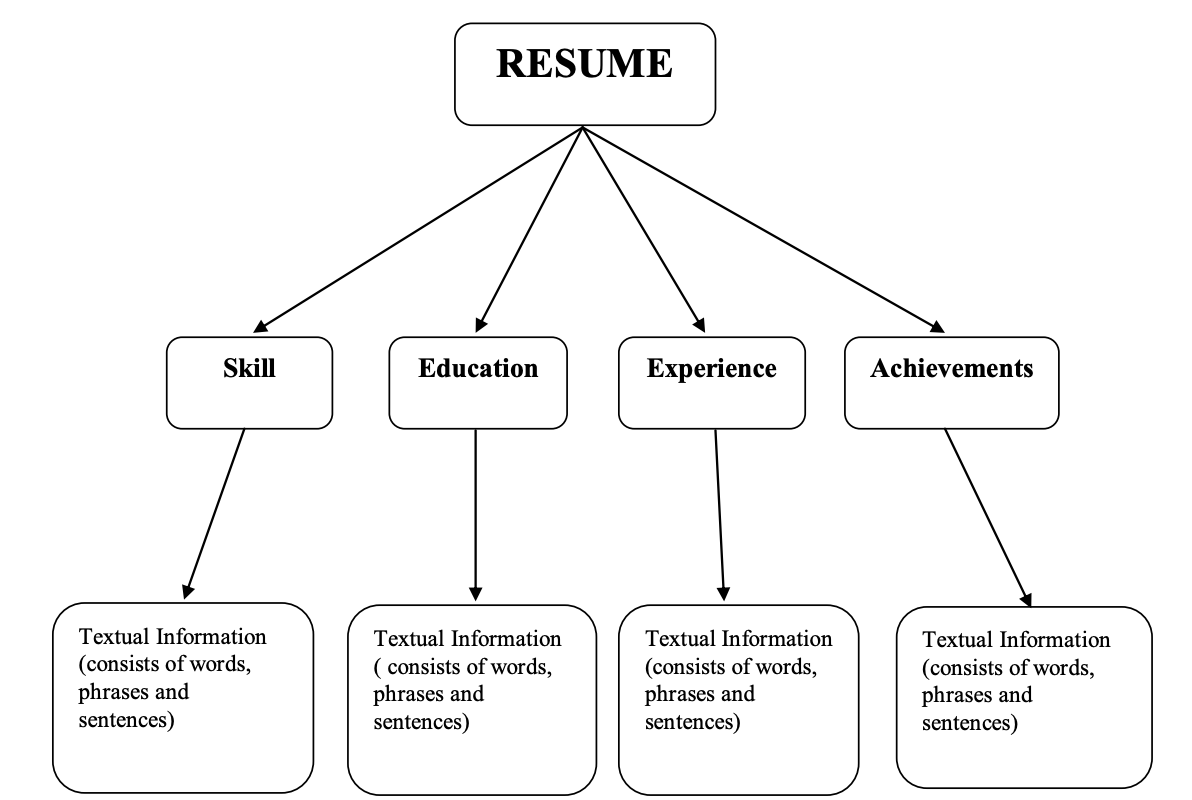
\includegraphics[width=0.9\textwidth]{images/resume_structure.png}
    \caption{Hierarchical Structure of Resume \cite{kudatarkar2015survey}}
    \label{fig:2}
\end{figure}



\section{NLP Techniques}

Natural Language Processing, also known as computational linguistics, is a subarea of computer science which uses computational approaches to learn to comprehend and produce natural language, and has proliferated over the past decades \cite{hirschberg2015advances}. NLP techniques are normally used to handle communication, including lexical, syntax and semantic analysis \cite{alamelu2021resume}. Before this project, there have been many implementations using NLP techniques to process resumes. \cite{alamelu2021resume} created a web application to help the resume screening process more accessible and straightforward. This web application can compare the submitted resumes with the job description and then rank resumes by the matching rate to find the candidates for the job. A modified NER (Named Entity Recognition) model is used to identify the crucial items in resumes, such as skills and work experience, and Cosine Similarity could compute the matching rate. 

Keyword extraction is also a vital process to understand the resumes better. Extracting keywords is complex because natural language is diverse and the concept of keyword is hard to define \cite{firoozeh2020keyword}. Hussey, Williams and Mitchell proposed a study on the comparison of automatic keyphrase extraction method \cite{hussey2012automatic}, which focuses on the extracted performance and result of different features. Moreover, Hasan and Ng researched the errors of the keyphrase extraction system \cite{hasan2014automatic}. As for the extraction features of resumes, the keyword extractors might be different from other systems. Though almost all resumes have unique structures, there can be found a typical hierarchical layered structure for resumes \cite{finn2004multi}, which can make the keyword extraction task for resumes easier. 

Kopparapu and Kumar \cite{kopparapu2010automatic} proposed a system to extract resume information automatically. This system can extract six different necessary informative fields, such as work experience, e-mail address and skill set, from the unstructured resume data by a series of NLP techniques, and can handle resumes in multiple forms. The extraction processes are implemented by part heuristics and part pattern matching techniques, which can be used in our project.
 \begin{figure}[H]
    \centering
    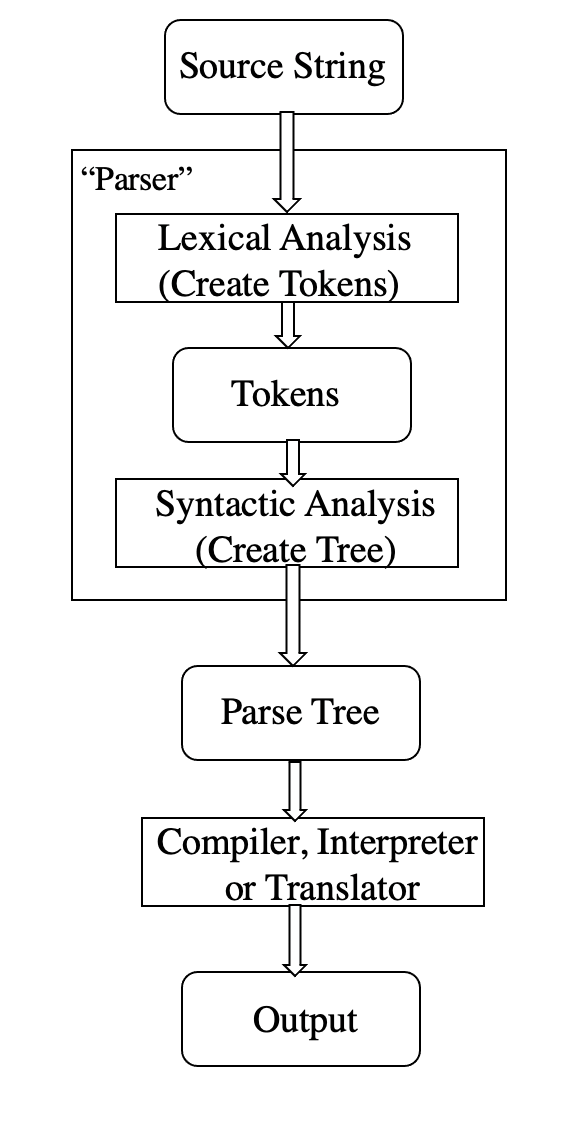
\includegraphics[width=0.35\textwidth]{images/model.png}
    \caption{Model Design \cite{sanyal2017resume}}
    \label{fig:1}
\end{figure}


Sanyal et al. \cite{sanyal2017resume} designed a model to parse all the relevant data in resumes including contact information, education details and work experience, and transform them into JSON format. The parser used Lexical Analysis, Syntactic Analysis and Semantic Analysis these three NLP techniques to constrain the information in the resumes. The Lexical Analysis part tokenized the input resumes data, and then used NER to extract the related information in each segment. The parser generated the parse tree, which can represent and directly reflect the syntax of the input data, through Syntactic Analysis. As for Semantic Analysis, it could study the meaning and the structure of the data, and could find the language-independent meanings. After three analyzers, the system will generate JSON data to represent the resume and store it in the database for further analysis. The model design is shown in the above figure \ref{fig:1}, which would be helpful for our project.



Identifying the features such as skills in the resume is another key point in a CV checker. An ontology-based resume searching system is developed to match CVs and job descriptions \cite{phan2021ontology}. Resume Ontology includes classes, properties and relational concepts, which can represent the resume in a semantic way \cite{ccelik2013towards}. Computer Science Ontology (CSO) Classifier is an unsupervised method that can take the metadata as the input and return the topic category of the document according to CSO \cite{salatino2019cso}. Phan et al. \cite{phan2021ontology} 's system can parse and processes the uploaded CV, extract the skills by CSO Classifier and match the CV to the target position by the calculated similarity of the skill graph. Figure \ref{fig:3} illustrates the process of the architecture of this Resume Searching system, and the design of our project could be referred to it.

 \begin{figure}[H]
    \centering
    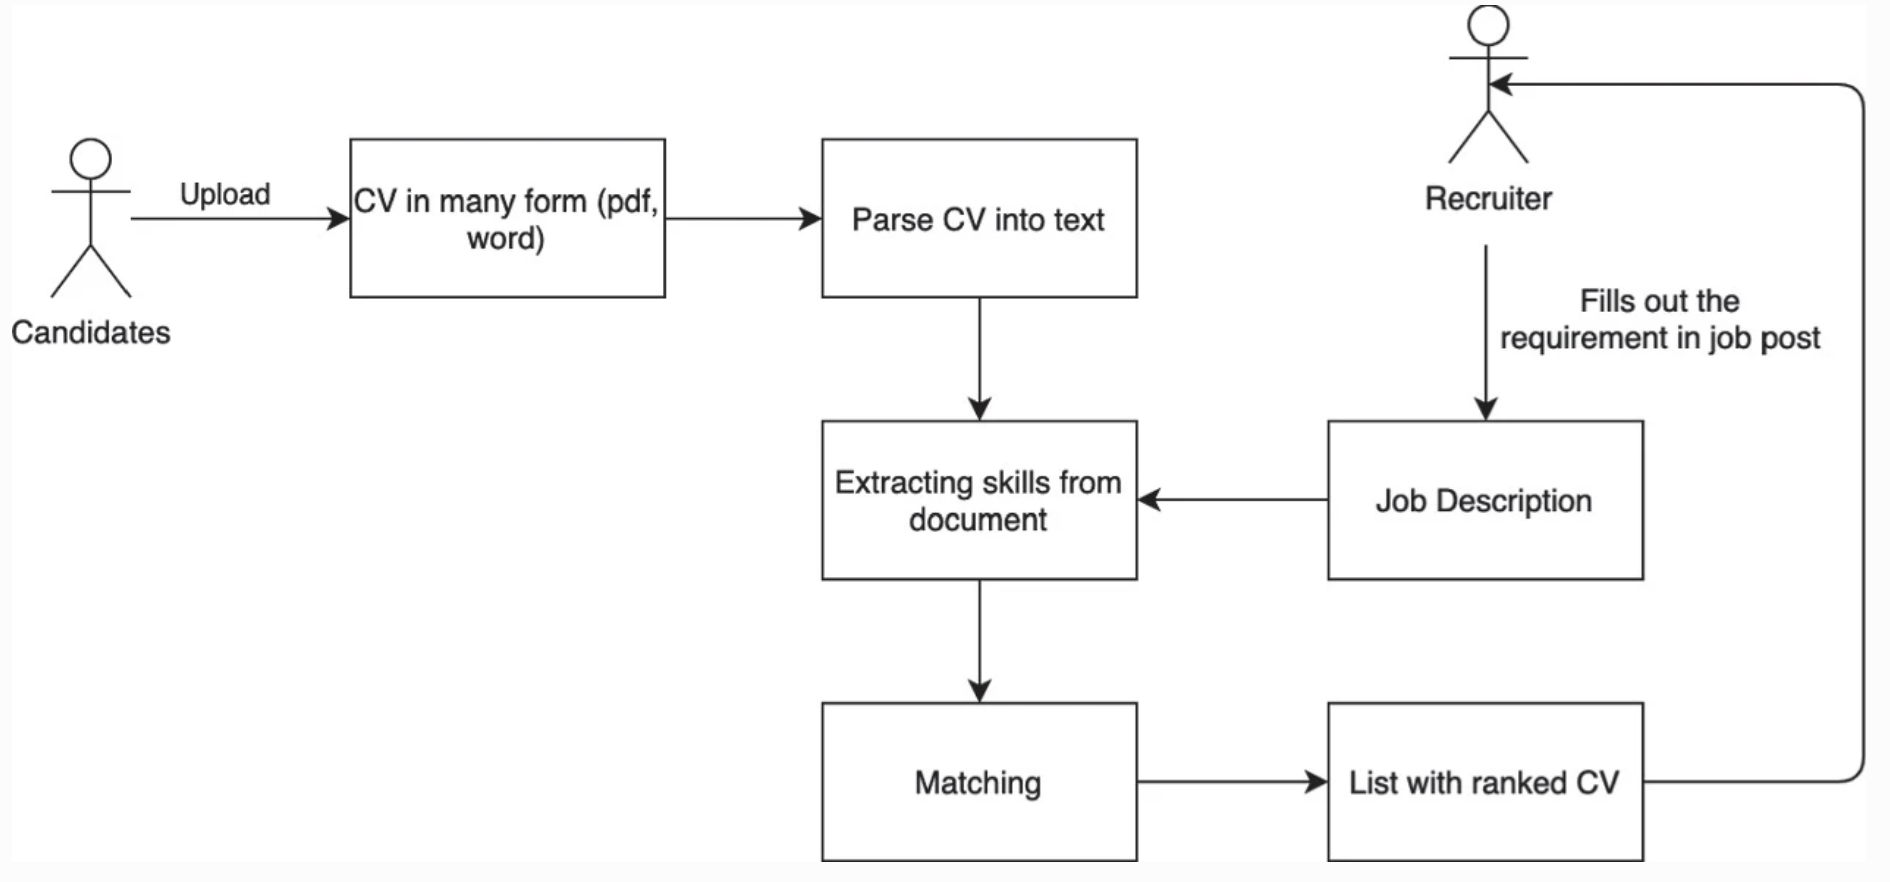
\includegraphics[width=0.9\textwidth]{images/architecture.png}
    \caption{Architecture of the Resume Searching System \cite{phan2021ontology}}
    \label{fig:3}
\end{figure}


In \cite{maheshwari2010approach}, an approach has been proposed for special skill extraction for companies to filter resumes and reduce the number of candidates. It can extract the skill type features and the skill value features, then calculate the specialness value degree of those features to determine and organize the particular skill type. The features could be organized into three levels, common features, common cluster features and special features by setting a similarity threshold value. This proposed framework can help the user or the recruiters to check the resume based on special skill type and get the corresponding skill values. This system is more likely to be used for selecting the suitable resume from a set of similar resumes on the basis of special skills. However, some ideas in it such as skill classification could be considered in our CV checker. 


\section{Machine Learning Techniques}

The machine learning algorithm, regarded as a part of artificial intelligence \cite{enwiki:1103198106}, can build the model based on the sample data to make predictions or decisions without specific program \cite{koza1996automated}. Techniques based on machine learning are widely used in various areas in which it is hard to be implemented by the traditional algorithm for the tasks such as medicine and speech recognition \cite{hu2020voronoi}. Nowadays, machine learning approaches are ubiquitous in NLP tasks, and have been proved to perform well on tasks such as Part of Speech tagging, Named Entity Recognition and Sentiment Analysis \cite{socher2012deep}. According to \cite{sinha2021resume}, it is a difficult task to extract information from human language since human language is diverse and ambiguous, and it can be expressed in many different ways. Machine learning models play an important role in reducing ambiguity and capturing linguistic information from the human language \cite{jurafsky2000speech}. Before using ML techniques, NLP tasks are implemented by rule-based approaches and should be coded manually \cite{khan2016survey}. Khan et al. \cite{khan2016survey} reported a comprehensive survey in machine learning and NLP domain to discuss different existing ML models applied in computational linguistics for disambiguation. 

Machine learning algorithms can also be used to analyze unstructured resume data. Sinha et al. \cite{sinha2021resume} discussed and evaluated several machine learning techniques for resume parsers. Those CV parsers analyze the context of the document by semantic search to obtain reliable and comprehensive results \cite{sinha2021resume}. Sentence segmentation is a vital task in order to extract definite information from the CVs. The rule-based approach uses a set of punctuations such as '.',';','?' to detect the boundary of the sentence \cite{reynar1997maximum}, but when encountering special situations such as abbreviations, it will be failed \cite{kiss2006unsupervised}. Under these circumstances, supervised machine learning methods such as decision tree could be used to classify the punctuations and decide the sentence boundaries more accurate \cite{riley1989some}. Generally, supervised learning needs to be provided input and output by human, and involves a large set of labelled training data to obtain a good performance \cite{saravanan2018state}. An unsupervised approach was proposed by Kiss and Strunk \cite{kiss2006unsupervised}, which used type-based classification for sentence segmentation by analyzing and annotating the word in the full text. Additionally, besides segmenting the sentences, statistical approaches could also be used in the tokenization task. The statistical approach used scanning hidden Markov model (HMM) boundary detector modules to tokenize \cite{jurish2013word}. Above is the usability of machine learning methods in the textual data processing. 

In e-recruitment, machine learning techniques are widely used to screen, classify and rank applicants automatically. Tejaswini et al. \cite{tejaswini2021design} used K-nearest Neighbours (KNN) algorithm to calculate the distance between resumes and the target job description and return the top K resume choices. \cite{vamsi2021resume} used Naive-bayes and one-vs-rest classifier to process and segregate resumes on the basis of knowledge and technical expertise. Ali et al. \cite{ali2022resume} evaluated nine ML models on Resume Classification System (RCS), and the Support Vector Machine (SVM) classifier got the best performance with over 96\% accuracy on the resume dataset. The results indicated that NLP and machine learning techniques could be used to develop the efficient RCS \cite{ali2022resume}. In our project, ranking or classifying resumes would not be involved, but the idea that combining NLP with machine learning approaches in resume-related projects could be taken into consideration.

Deep learning is a subfield of machine learning which aims to develop high-level features and representations from the complex explication input by multiple layers \cite{deng2014foundations}. \cite{gunaseelan2020automatic} proposed a system that can extract information such as skills, education and experience from the resume by a multi-level classification approach. Ontology matching technique can be used to recognize the technical skills by part of speech patterns, but it relies extremely on the completeness of the database \cite{chifu2017system}. In this situation, with the development of computational ability, deep learning models such as LSTM are used for Named Entity Recognition for segment information extraction \cite{gunaseelan2020automatic}. \cite{chen2018two} implemented a text block classification method by regarding the text as blocks based on the title words of the resume documents. But since the unstructured characteristic of resumes, it is complicated to define this kind of document as separate blocks. Ayishathahira et al. \cite{ayishathahira2018combination} used Convolutional Neural Network (CNN) segmentation model to segment the information into educational, occupational and others, and CRF and BiLSTM are developed for information extraction. \cite{kumar2019supervised} came up with a supervised deep learning algorithm regarding the skills as relevant keywords to extract skills from the resume by predicting the relevant keywords. The importance of each word in the data are calculated to indicate the probability of a word being the skill.

Many other machine learning algorithms other than deep learning approaches could be used for the above skill extraction task. \cite{jo2017using} used K-Nearest Neighbors for text segmentation, which calculates the similarity among the feature vectors and classifies the sentences into specific groups based on the similarity. Ensemble learning combines multiple learning algorithms together to obtain better performance than a single learner \cite{enwiki:1100411098}. \cite{goudjil2018novel} proposed a multi-class SVM approach to learn the knowledge of the data by selecting the most informative samples. 

In addition, identifying the skills in the job description to check the resume is regarded as a significant task in the CV checker as well. Liu et al. \cite{liu2021learning} proposed a Multi-Graph Neural Network based Skill Prediction (MGNSP) model to define the job skill requirements for the positions. They built three networks for job, skill and job-skill to get the recommended skills for a job position. Job network can aggregate the information from the neighbors of every job description to handle the false predictions, Skill network models the skills' correspondence and Job-Skill network combines the job descriptions and skills together to get the suggested skills from the similar descriptions of the position. The prediction of skills would not be used in this project, but the three networks to get the aggregation and correlation could help to understand the job description data. Like the unstructured resume data, deep learning models such as LSTM and biLSTM are able to recognize the skills expression from the job posts based on time series data \cite{baad2019automatic}. Moreover, Zhou et al. \cite{zhou2016quantifying} adapted a systematic method to measure the relevance of the skills to the job titles depending on the job description and skill keyword representation. In their research, the skill relevance is assessed by TF-IDF (Term Frequency - Inverse Document Frequency) based score and the dispersion of the skill expression over the positions. The above approaches, such as skill ranking and skill relevance across the job description could be considered as the future work for our project.
\chapter{Methodology \& Theory}
% \addcontentsline{toc}{chapter}{Methodology}
\label{ch:methodology}

This chapter will illustrate the main technologies used in the project. From the web development frameworks, data preprocessing steps, to back-end algorithms, the tools and methodologies that used during the development will be described in detail.


\section{Web Development}

Web is one of the most wide-used networking aids that can fulfil all kinds of user requirements and provide the solution to different problems \cite{lokhande2015efficient}. To develop a well-structured Web application, a suitable technology should be used \cite{lokhande2015efficient}. There are a large number of standard libraries in python that can make web development simple, and Django and Flask frameworks are two popular and frequently-used Web application frameworks. According to \cite{ghimire2020comparative}, Flask is flexible and straightforward controlled, which is easy and quick to learn, while Django is easy to work with because of the substantial libraries and features. 

In this project, the Flask framework in python is chosen to implement the Web application. It provides needed tools, libraries and technologies for back-end development. Flask was developed based on Werkzeug WSGI toolkit, which implements a simple HTTP server and reduces the workload of Web framework development. The structures of Flask can be divided into Static files and Template files \cite{lokhande2015efficient}. The static file contains CSS and JavaScript codes that are the static codes for the website, while the template file has the Jinjia templates for the dynamic page. Additionally, Flask is open-sourced and developers can modify the source code for further design.

In addition, there are many frameworks and libraries for front-end web development, which have helped to promote the development of front-end \cite{dinh2020modern}. In recent years, JavaScript frameworks have made the UI developer more powerful and productive, and React.js, Angular.js and Vue.js are three popular JavaScript front-end frameworks. Vue framework is said to have a high degree of encapsulation and is easy to start because it is simple and reasonable. Vue.js provided data-driven and component-based development by Model View View-Model (MVVM) pattern \cite{li2021research}, which aims to separate the data layer (Model) and UI presentation layer (View), then using ViewModel to achieve the inside logic \cite{anderson2012model}. The following Figure \ref{fig:4} shows the MVVM construction of Vue. Moreover, Vue provides a re-rending feature, because of which most developers prefer to choose Vue.js as the framework \cite{novac2021comparative}. Due to the above advantages, in this project, Vue.js is chosen as the front-end framework for UI development.

 \begin{figure}[H]
    \centering
    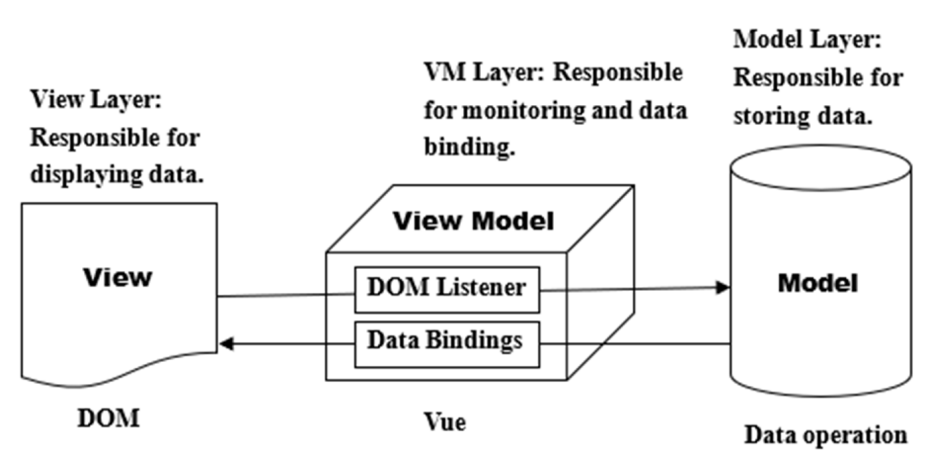
\includegraphics[width=0.6\textwidth]{images/MVVM.png}
    \caption{MVVM Architecture of Vue \cite{li2021research}}
    \label{fig:4}
\end{figure}


\section{CV Parser \& Data Preprocessing}
\label{method_preprocessing}


This section will introduce the technologies for the general parsing processes of unstructured text data and the preprocessing steps in NLP.

The general analysis steps of NLP are shown in Figure \ref{fig:5}, including Lexical Analysis, Syntactic Analysis, Semantic Analysis, Discourse Analysis and Pragmatic Analysis.

 \begin{figure}[H]
    \centering
    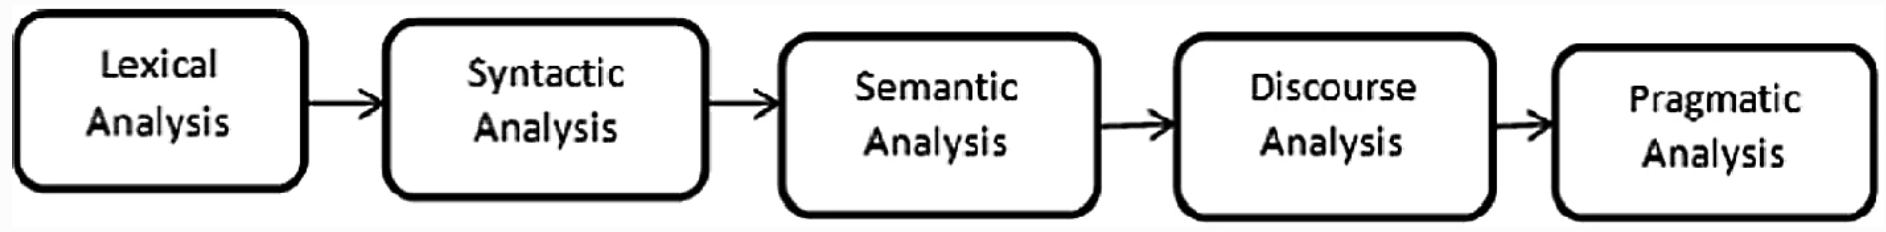
\includegraphics[width=0.8\textwidth]{images/preprocessing_step.png}
    \caption{Analysis Stages in NLP \cite{yogish2018review}}
    \label{fig:5}
\end{figure}

Lexical Analysis is the process that can transform a sequence of characters into tokens \cite{enwiki:1077694767}, which is the first stage of the resume parser. The first phase of the Lexical analyser is scanning, which can divide the input data into syntactic units and categorise them. The second phase is evaluating, which can convert the units into computer-readable values. In our project, the Lexical analyser can be used to parse the input resume to tokens for further processing. As for the second stage of the resume parser, Syntax Analysis takes the input in the form of token streams from the Lexical analyser to parse the code and confirm the rules and the structure of the grammar, then output a parse tree \cite{smith_2022}. A sequence of strings consists of phrases, sentences and paragraphs, and Semantic Analysis is the process related to extracting the structure and language-independent meanings of the sequence. \cite{enwiki:1062314320}. Semantic Analysis can start with the relations between each token to understand the lexical hierarchy such as hyponymy, hypernymy, synonyms and antonyms \cite{manning1999foundations}. In this project, Semantic Analysis can learn the language-independent meanings in the resumes. For example, if the education information from resume A is graduated from 'University of Manchester', and in resume B is 'Manchester University', the Semantic analyser can convert the 'University of Manchester' to 'Manchester University'.

There are many available tools for NLP preprocessing tasks, such as Gensim, NLTK (the Natural Language Toolkit) and Spacy. The comparison of numerous NLP toolkits is shown in Table \ref{tbl:1}. NLTK is a platform to support programs dealing with natural language data, which is regarded as a suitable tool for education, programmers and researchers, and easy to get start with. According to \cite{yogish2018review}, NLTK provides many grammar collections, corpora and trained models for real world data, and comes with many beneficial functions for common NLP tasks. In this project, NLTK is chosen as the toolkit for the data preprocessing tasks.

\begin{table}[htbp]
\centering
\begin{tabular}{|c|c|c|c|c|c|}
\hline
NLP toolkit & Tokenization & POS tagging & Chunking & NER & Stemmer \\
\hline
NLTK & Yes & Yes & Yes & Yes & Yes \\ 
\hline
Apache OpenNLP  & Yes & Yes & Yes & Yes & Yes \\
\hline
Stanford CoreNLP  & Yes & Yes & No & Yes & Yes \\
\hline
Pattern  & Yes & Yes & Yes & No & No \\
\hline
GATE & Yes & Yes & Yes & Yes & No \\
\hline
Spacy  & Yes & Yes & Yes & Yes & No \\
\hline

\end{tabular}
\caption{Comparison of NLP Toolkits \cite{yogish2018review}}
\label{tbl:1}
\end{table}

After parsing the raw text data, the first step is clean the data by removing special characters, carriage returns and line breaks. With the cleaned data, NLP preprocessing tasks could be applied to convenient the subsequent machine learning algorithms. Tokenization is the early step in the NLP pipeline, which is the method that splits the text into tokens. Words, phrases and sentences can all be regarded as tokens, where the word is a token in the sentence and the sentence is a token in the paragraph. NLTK provides several ways to tokenize text. PunktSentence tokenizer can be used to tokenize the text into sentences, and WordPunct tokenizer is based on regular expressions to separate the text by space and punctuation. Additionally, the Treebank tokenizer also uses regular expressions with Penn Treebank corpus to tokenize text, which can separate standard contractions, regard punctuation as the individual token, and split full stops at the end of the sentence. 

Stop word removal is the next widely used method in NLP preprocessing. Words like "the", "a", an "in" occur in all documents frequently and are considered the stop words, which should be removed since they do not contain useful information for further analysis. According to \cite{raulji2016stop}, removing stop words can be applied to strengthen the performance of Information Retrieval System, Text Analytics and Text Summarization tasks. NLTK provides a list of the most common stop word for stop words removal without defining the stop words manually.

 \begin{figure}[H]
    \centering
    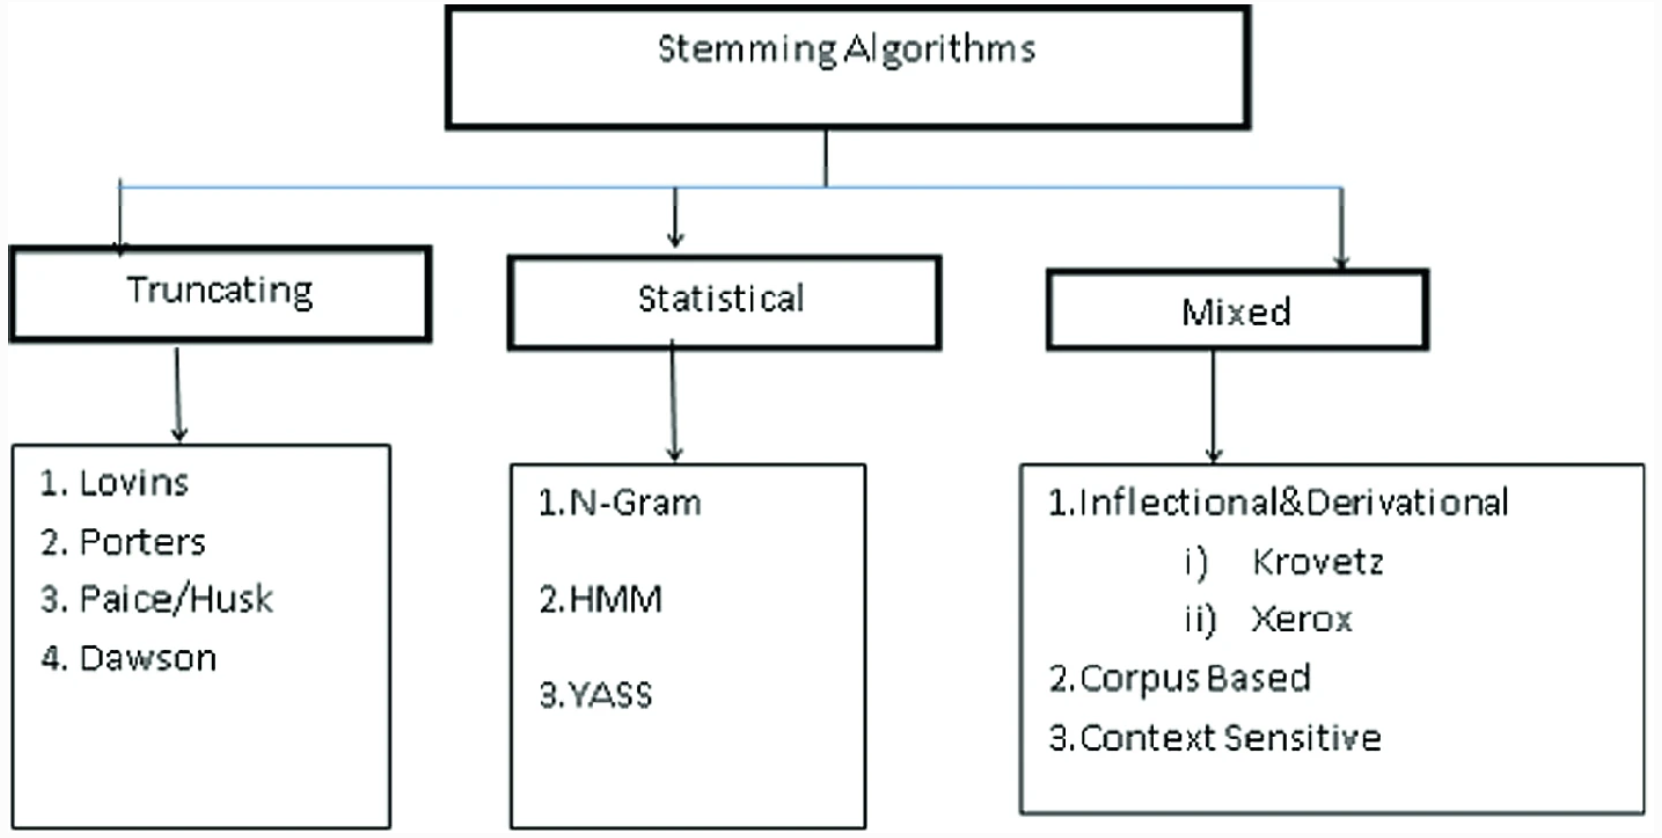
\includegraphics[width=0.9\textwidth]{images/stemming.png}
    \caption{Stemming Algorithms \cite{yogish2018review}}
    \label{fig:6}
\end{figure}

Stemming is a significant preprocessing step that transforms the inflected words to their root form in order to cut down the size of index and increase the accuracy of retrieval. Figure \ref{fig:6} shows the classification of the stemming algorithms. Truncating methods can remove the affixes of the word to build the stem; statistical methods use statistical analysis to produce stem, and stemmers in mixed methods are developed relying on the inflectional and derivational morphology \cite{yogish2018review}. In NLTK, there are several different stemmers such as PorterStemmer, LancasterStemmer and SnowballStemmer. PorterStemmer is one of the most commonly used stemmers, and the output stem is always the short word with the same root meaning.


Lemmatization is the process of gathering the inflected forms of a word so that they can be regarded as a single unit for analysis \cite{enwiki:1100992412}. The lemmatization process is highly close to stemming but includes the intended meaning of a word, which aims to discover the normalized form of the word. For instance, the lemma of the word "better" is "good". NLTK contains the method WordNetLemmatizer() to lemmatize a word by its context and usage in the sentence, which can be used for text understanding, clustering, tokenization and visualization. 

Part of Speech (POS) labelling is another vital preprocessing method that assigns the part of speech tags for each word in a sentence, where POS is a kind of grammatical feature including nouns, verbs, adjectives, et cetera. According to \cite{kumawat2015pos}, POS tagging is known as a necessary tool for numerous NLP activities, like word disambiguation, information recovery, and machine interpretation. The following Figure \ref{fig:7} shows the process of POS tagging, where the tagging algorithm allocates the tags to individual tokens and compares them with the tag set. There are rule-based, stochastic, and hybrid approaches for POS tagging. Rule-based tagger searches the dictionary and returns all the possible tags, then removes ambiguous words using the linguistic features by hand-coded rules to get the single POS tag of a word \cite{yogish2018review}. In contrast, the stochastic tagger assigns the tags by probability and statistics based on corpus evidence. The hybrid approach combines the rule-based and statistical methodology together \cite{rathod2015survey}, which uses hand-coded rules to illustrate the tags and applies statistical machine learning methods to induce rules from the training corpus. NLTK POS tagger uses the Penn Treebank tag set as default and the maximum entropy model to generate the tagged corpus.

 \begin{figure}[H]
    \centering
    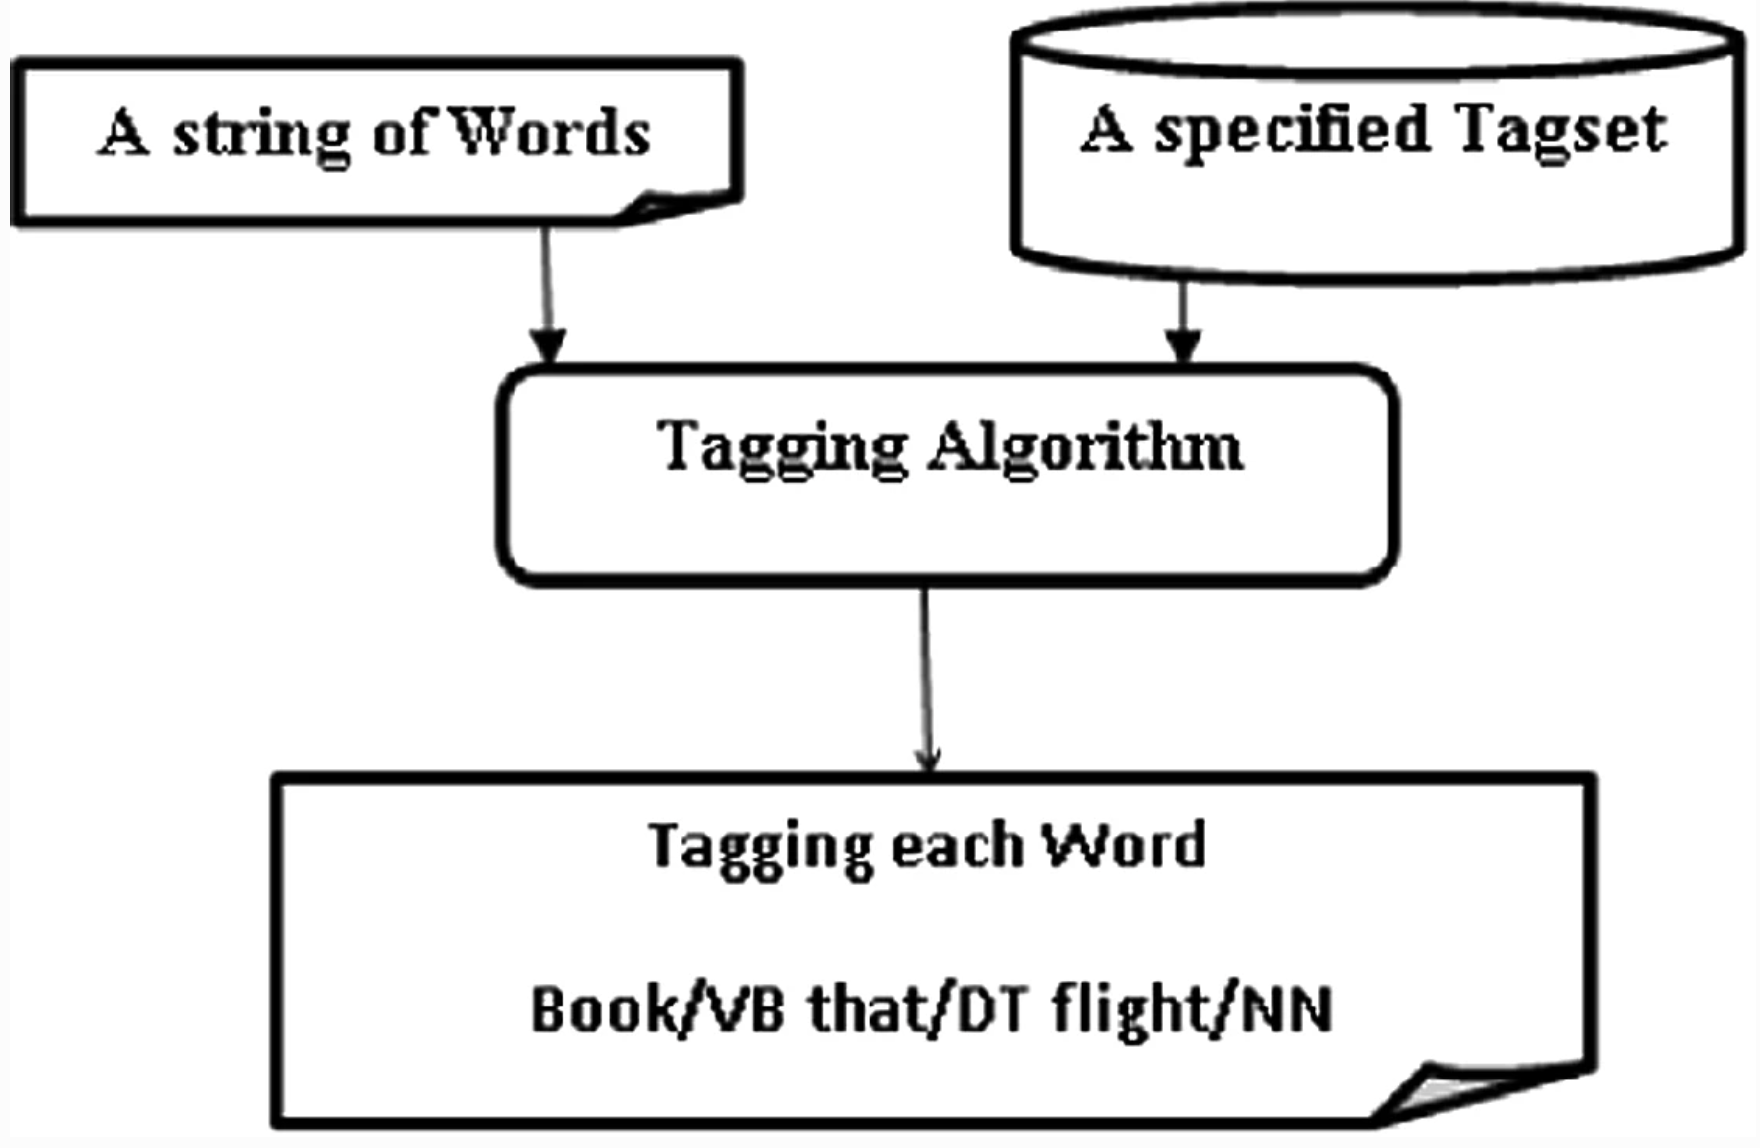
\includegraphics[width=0.5\textwidth]{images/POS.png}
    \caption{Process of POS Tagging \cite{yogish2018review}}
    \label{fig:7}
\end{figure}



\section{Related Techniques}
As illustrated in Chapter \ref{ch:background}, NLP and machine learning techniques would be used to achieve the resume-checking function. This section will describe the methods and tools related to the back-end algorithms separately, including information recognition, skill extraction, and skill matching.

\subsection{Information Recognition}
% NER / profile info / skill extraction (clustering, topic modeling, Bert)
% word embedding

Checking the integrity of personal information in the resume is one of the main tasks for this CV checker, which means the information such as name, e-mail address, education and work experience should be recognized by the back-end algorithms. Named Entity Recognition (NER) can be used as the tool for this task.


NER can implement the information extraction task by locating and classifying real-world objects or proper nouns in unstructured text data. Pre-defined categories such as organizations, locations and persons can be recognized in the text data by NER, and many applications like Information Retrieval System \cite{khalid2008impact} have been improved on account of the usage of NER. According to \cite{mohit2014named}, there are two sub problems of NER, one is named entity boundaries' recognition, and the other is the categories recognition. Dictionary-based, rule-based and machine learning-based are the three approaches of NER. The dictionary-based approach can match features by dictionary looking up, which is a simple method and can obtain good precision. Nevertheless, this hand-crafted-based system requires a massive effort by domain experts to build the dictionaries and is said to have difficulty in complete coverage for many named entity categories \cite{neelakantan2015learning}. The rule-based method uses rules and patterns of named entities which can consider the context of the entities, but the rules should be written before recognition. For this project, the information that needs to be extracted is personal information instead of proper nouns. Therefore, the dictionary-based and rule-based approaches are unsuitable since it is hard to write the common rule set for the entities.

Machine learning-based methods utilize statistical models to recognize the named entities in the text. Hidden Markov Models (HMMs), Conditional Random Fields (CRFs) and Neural Network models can be applied to the NER problem. CRFs is a discriminative sequence framework for sequence labelling, which aims to find the most probable label sequence $y^*$ given the observation sequence $x$ \cite{lafferty2001conditional}, 

\begin{equation}
    y^* = \mathop{\arg\max}{_yp(y|x)}
\end{equation}

where $x$ consists of the sequence of the input tokens. The computation of probability is as follows, where $w$ refers to the weight, $f$ is for the feature function, $T$ refers to the summation of all tokens and $K$ means the summation over all feature functions \cite{lafferty2001conditional}:

\begin{equation}
    p(y|x) = \frac{1}{Z_x}\exp(\sum_{t=1}^{T}\sum_{k=1}^{K}w_kf_k(y_t,y_{t-1},x_t))
\end{equation}

CRFs models can be approximately interpretable and do not need pre-trained vectors. However, it performs prediction using input features, which means feature engineering should be completed before training. Neural networks can handle the sequence processing problem without feature functions, which can detect implicit features from the input data automatically by hidden layers. Take BiLSTM as an example, the feature function in CRFs can be replaced by:

\begin{equation}
    f(tag_i, tag_{i-1}, token_i) = Wh_i + b
\end{equation}

In this project, spaCy is used for the NER task, which is an application-oriented, open-sourced library for NLP. SpaCy supports deep learning workflows, allowing its deep learning library Thinc to connect statistical models trained by other machine learning libraries such as TensorFlow \cite{enwiki:1094217869}. Thinc is a lightweight deep learning library powering spaCy, with which, as the back-end, Convolutional Neural Network (CNN) models can be applied in spaCy to advanced NLP tasks such as POS tagging and NER. With spaCy, developers do not need to take time to build or adjust the neural network structure because spaCy provides the most advanced neural network framework for NER model training instead. According to the official document of spaCy \cite{honnibal_2022}, the NER system presents a highly-developed word embedding approach. It uses the features of subword and Bloom embedding, a Convolutional Neural Network with residual connections, and a transition-based method for named entity parsing, where bloom embedding is an approach that can reduce the model size of NER. This system is developed to balance the efficiency, accuracy and flexibility of NER model training. With a normalized training dataset containing named entity tags, the spaCy NER model can be trained and used to recognize the pre-defined named entities in the new input data.

\subsection{Skill Extraction}

Extracting skills from the resume and the job description data is another main task for the back-end algorithm. NER can also be utilized for skill extraction if suitable training data exists with named entity labels. Otherwise, techniques like clustering algorithms, topic modeling and Bidirectional Encoder Representations from Transformers (BERT) could be considered utilized for the skill extraction task from text data.


The basic idea of using clustering algorithms to extract skills in a document is regarding the word vectors as the samples and gathering them into different groups, which are expected to have one or more clusters indicating to different kinds of skills. 

\subsubsection{Word Embedding \& K-means Clustering}
\label{sec:word2vec}

Before clustering, word embedding techniques should be used for the representation of words in the form of vectors. Word2vec is an approach that can learn the correlation among words from the corpus by neural network and represent each word as a vector. Based on a word's usage in the text, word2vec can infer the meaning of the word with a high level of accuracy. The output is vectors for each word with remarkable linear relationships, which can be calculated like \cite{mikolov2013efficient}:

\begin{equation}
    vec("king") - vec("man") + vec("woman") =~ vec("queen")
\end{equation}

The assumption to get the words' representation is: 1) there is a vector $v \in R^d$ to represent each word $w \in V$; 2) there is a probability $Pr(w|u_1,u_2,...,u_l)$ for the word $w$ appears in a context $(u_1,u_2,...,u_l)$. The task is to find the vector $v$ that can maximize the probabilities for each word $w$ and the context $(u_1, u_2,...,u_l)$, where neural network parameters can be used to compute the probabilities by minimizing the cross-entropy loss.

Continuous bag-of-words (CBOW) and Skip-gram architectures are utilized in Word2vec to generate the distributed word vectors. CBOW model predicts a word from the surrounding words with the architecture shown in below Figure \ref{fig:8}:

 \begin{figure}[H]
    \centering
    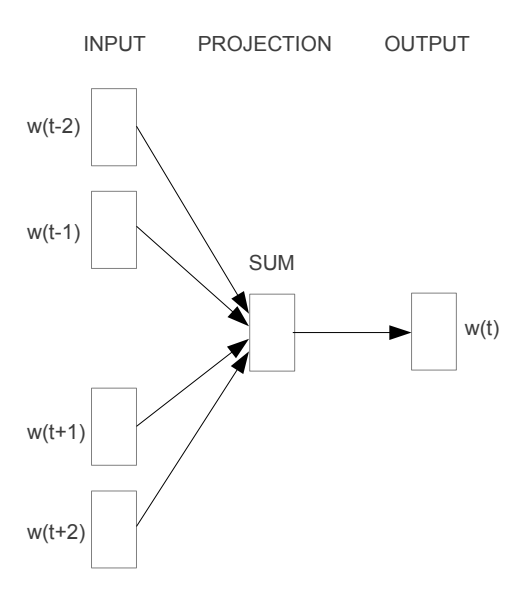
\includegraphics[width=0.35\textwidth]{images/CBOW.png}
    \caption{Model Architecture of CBOW \cite{mikolov2013efficient}}
    \label{fig:8}
\end{figure}

where the probability $Pr$ of word $w_t$ appears in its context $(w_{t-1},...,w_{t-m+1})$ is:

\begin{equation}
    Pr(w_t|w_{t-1},...,w_{t-m+1}) = softmax(Wy)
\end{equation}

\begin{equation}
    y = average(w_{t-1},...,w_{t-m},w_{t+1},...,w_{t+m})
\end{equation}

In contrast, Skip-gram uses a neural network model to predict contextual words instead of a target word, and the structure of the model is shown in the following Figure \ref{fig:9}. According to \cite{mikolov2013efficient}, Skip-gram performs well with a small amount of data and is effective at representing uncommon words, while CBOW is faster and more suitable for representing frequent words.

 \begin{figure}[H]
    \centering
    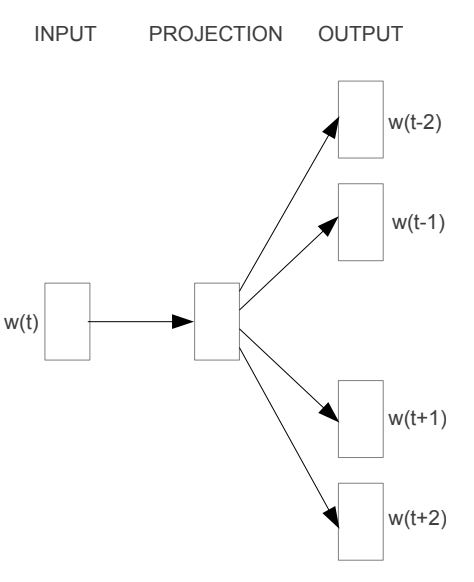
\includegraphics[width=0.35\textwidth]{images/skip_gram.png}
    \caption{Model Architecture of Skip-gram \cite{mikolov2013efficient}}
    \label{fig:9}
\end{figure}

Word2vec algorithm can be implemented by Gensim, an open-sourced library contains word2vec algorithm, latent semantic analysis and so on. Moreover, Gensim provides both CBOW and Skip-gram algorithms to train the model and get the word vectors. In this project, Gensim would be used as the tool to get the representation of the words for the subsequent clustering algorithm.

After getting the word embeddings, K-means algorithm can be used to partition the word vectors as the samples to get the expected skill clusters. K-means algorithm assumes that a given sample set could be separated into K clusters based on the distance between the samples and the centers \cite{macqueen1967classification}. The distance among the clusters is anticipated to be sufficient and the member points in each cluster are expected to be as close as possible to one another. Scikit-learn, a progressively popular machine learning library, provides the implementation of K-means algorithm, which will be used in this project to get meaningful clusters. With the trained clusters, each word in a new input document can be allocated to a suitable cluster, where those assigned to skill clusters are identified as skills in the text.


\subsubsection{Topic Modeling}
%Topic modeling
Besides K-means clustering algorithm combined with word embedding techniques, topic modeling is also a clustering tool for figure out the connection among text content. The skill vocabularies or phrases can be regarded as keywords in the job description. Topic Modeling techniques are expected to extract the important keywords by treating words in the corpus as features.


Unlike K-means, topic modeling is a probability-based algorithm using an unsupervised machine learning approach to identify word clusters through a set of documents. Latent Dirichlet Allocation (LDA) model is a classic topic model with a three-level hierarchical Bayesian model proposed by Blei et al. \cite{blei2003latent}, which applies Dirichlet distribution as the prior and estimates the posterior to infer the parameters by learning from the given document set. LDA assumes that each document is generated by potential topics and each topic is a probabilistic distribution over words. The graphical representation of LDA is as following Figure \ref{fig:10}, where $\alpha$ and $\beta$ are given parameters, $\theta$ is the joint distribution of a topic mixture, inner rectangle $N$ denotes the replicates of the selection of topics $z$ and words $w$ in a document, and outer rectangle $M$ represents the repeats of the document generation process \cite{blei2003latent}. And the purpose of LDA algorithm is to extract the latent topics in a set of the document by determining the probability that a word is associated with a topic and the proportion of a document that is related to a topic.

 \begin{figure}[H]
    \centering
    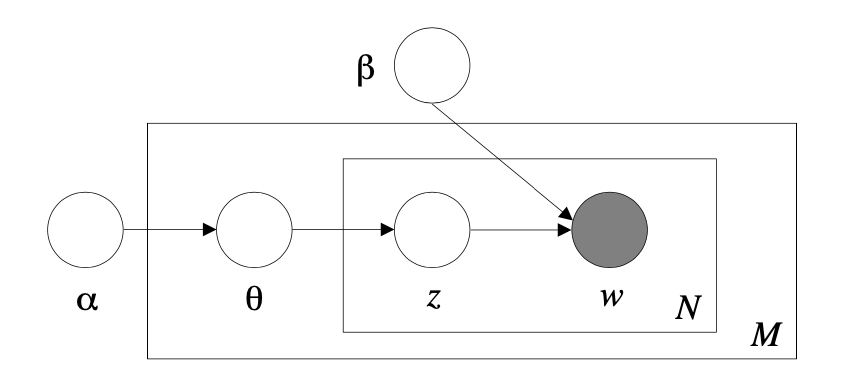
\includegraphics[width=0.5\textwidth]{images/LDA.png}
    \caption{Graphical Representation of LDA \cite{blei2003latent}}
    \label{fig:10}
\end{figure}

Gensim provides an optimized LDA implementation, which not only enables estimating the LDA model from the training corpus, but also can infer the topic distribution on new documents. The output topics are represented by the combination of top keywords in each topic with their weight. Additionally, the Gensim LDA module provides the perplexity and coherence score for the topic to evaluate the generated topic model. 

\subsubsection{Hybrid Approach}
\label{sec:hybrid}

Without a sufficient skill database, Some simple approaches might not produce the desired extraction result. In this situation, combining several NLP techniques and a machine learning-based classifier may perform better. Ketterer \cite{ketterer} proposed an approach that used POS, Chunking and a BERT Embedding classifier to identify the skills in the job description. The overall design of this hybrid approach is depicted in Figure \ref{fig:13}, where the regex (regular expression) chunking strategy is used to obtain the potential phrases, and the training set of the subsequent neural network is made up of the labeled extracted chunks.

 \begin{figure}[H]
    \centering
    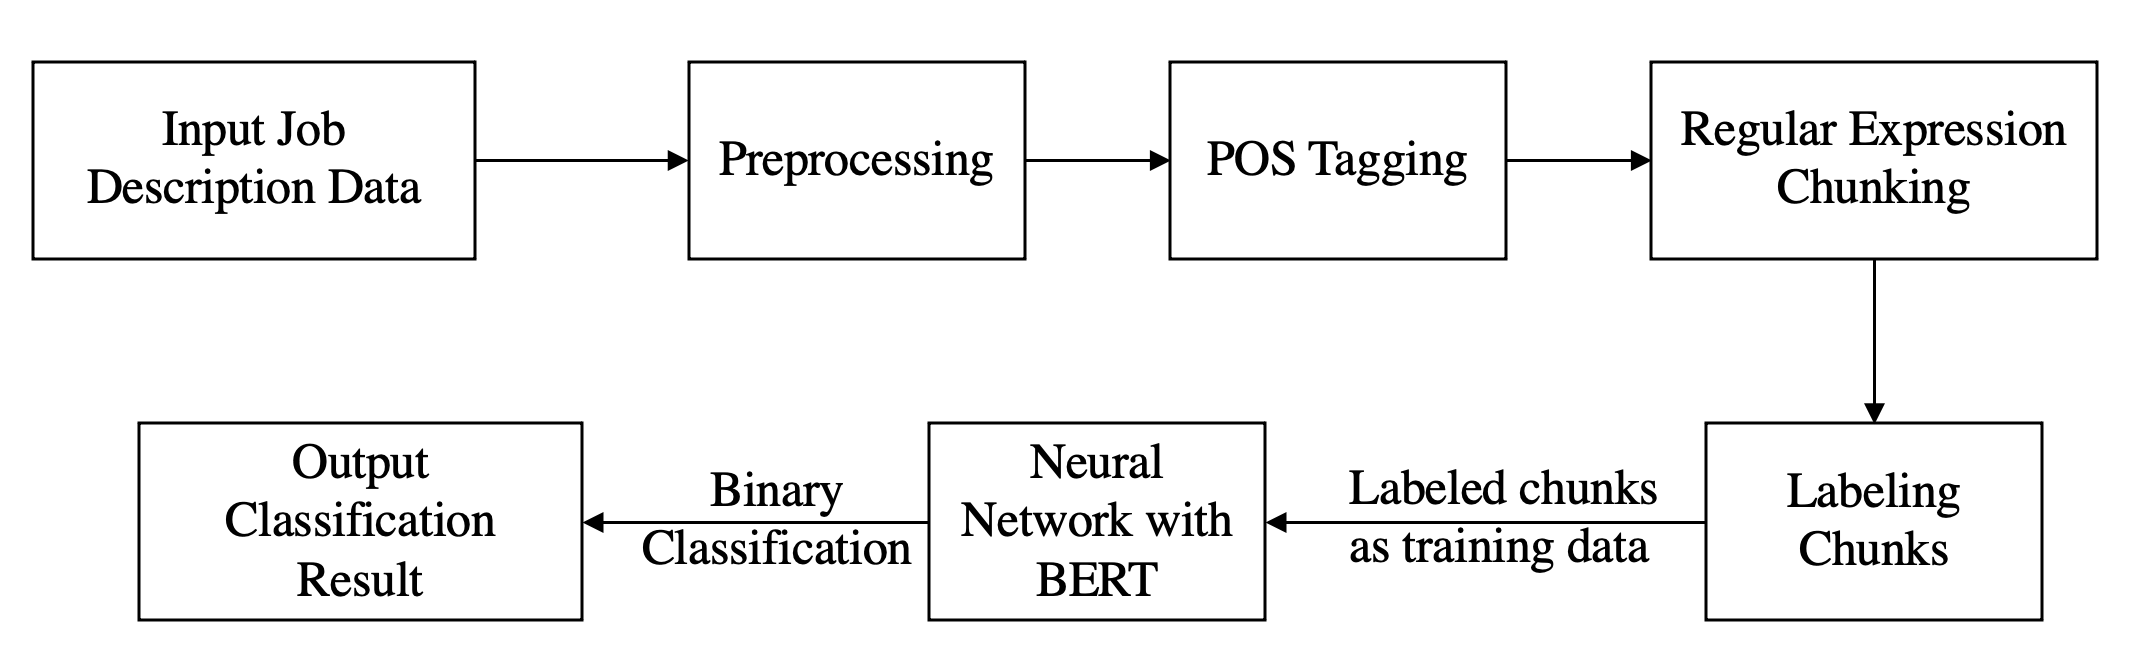
\includegraphics[width=0.85\textwidth]{images/Process.png}
    \caption{Overall Process}
    \label{fig:13}
\end{figure}


Preprocessing techniques and POS tagging are introduced in the previous sections, which are the first two steps in this model. Given the job description data, clean the dataset by tokenization, stemming, removing stop words and other preprocessing methods, then identify the Part of Speech in each job description for further analysis. 

POS tagger labels the individual words in the text with their probable Part of Speech. To understand the structure of the text and extract the patterns that might contain the skill expressions, Chunking should be used to determine certain phrases according to the words' POS combinations. The chunking algorithm takes POS tags as the input and outputs the chunks in the text. According to \cite{d'souza_2018}, Chunking is crucial when extracting Location, Organization, and Person Name information from the text. Similar to POS tag sets such as Penn Treebank tagset, phrase tags also have standard types like Noun Phrase(NP), Preposition Phrase(PP), etc. For the chunking process, NLTK provides a technique for the generation of chunks with the use of regular expressions. Ketterer defined four patterns' regular expressions for the phrases might hold the skill terms: Noun Phrase, Noun Phrase with preposition or conjunctions, Verb Phrase and Nouns between commas \cite{ketterer}. With these regular expressions, NLTK can extract the potential skill phrases to build the training dataset.

The extracted phrases are labeled to 1 (isSkill) or 0 (notSkill) manually, and a neural network are built to handle the binary classification of phrase samples. Transfer learning is a machine learning research subject that concentrates on storing knowledge obtained from one task and applies to the other related task \cite{enwiki:1099727359}, which means the pre-trained model can be regarded as a start point for a new model on different problem. Therefore, transfer learning enables the training process to depend less on the volume of data and results in better learning performance than training on a small dataset alone \cite{zhuang2020comprehensive}. Bidirectional Encoder Representations from Transformers (BERT) is a state of the art NLP model, which has been pre-trained by numerous corpora to produce better word embedding. With the advantage of word embeddings, BERT is used in this skill extraction task to generate significant robust, contextual understanding and semantic similarity word embeddings \cite{ketterer2}. The structure of the BERT layer is as follows.

 \begin{figure}[H]
    \centering
    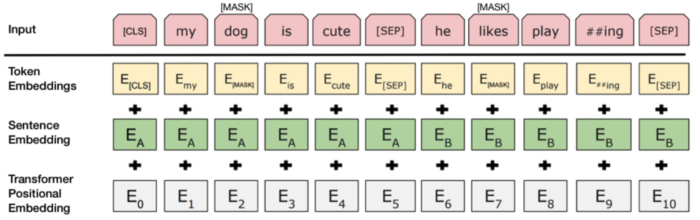
\includegraphics[width=0.85\textwidth]{images/BERT.png}
    \caption{Structure of BERT Layer \cite{ketterer2}}
    \label{fig:11}
\end{figure}

% Using the BERT layer, the architecture of the neural network is shown in following Figure \ref{fig:12}.

%  \begin{figure}[H]
%     \centering
%     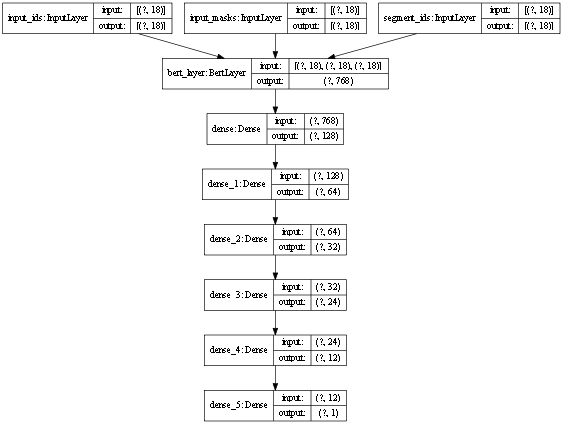
\includegraphics[width=0.9\textwidth]{images/withBERT.png}
%     \caption{Architecture of Neural Network \cite{ketterer2}}
%     \label{fig:12}
% \end{figure}

The trained neural network model enables to determine whether the phrase is a skill or not. When inputting an unseen job description, the text should be preprocessed, labeled with the POS tags and chunked. Then the neural network model with BERT layer is utilized to determine the skills in the extracted chunks.


\subsection{Skill Matching}

The match rate between resume and job description could be calculated using the extracted skills from both the two text, because in this project, skill matching is the most concerning part.

A straightforward idea to calculate the match rate is using semantic cosine similarity. Cosine similarity is measured by the cosine value of the angle between the text vectors to detect if they are pointing to a similar direction \cite{han2011data}, where larger cosine values denote smaller vectors' angles. Word embedding techniques like Word2Vec and TF-IDF (Term Frequency-Inverse Document Frequency) can convert the process from linguistic sentences to vectors. Word2Vec algorithm has been introduced in the previous Section \ref{sec:word2vec}, which is a prediction-based approach for word embedding, while TF-IDF is a count-based approach. The aim of TF-IDF is to emphasise terms that only appear in a few documents while weighing down the common words that are used in almost all documents. TF is the term frequency of a word, which means the count of the word appearing in one document, and IDF denotes the inverse document frequency, whose value would be smaller if the words occurred in the corpus frequently. The formulas for word $i$ in document $j$ are as follows:

\begin{equation}
    {TF_{i,\ j}=\ \frac{n_{i,j}}{\sum_{k}n_{k,j}}}
\end{equation}

\begin{equation}
    IDF_i=\log{\frac{|D|}{\{j\ :\ t_i\ \in d_j\}\ +\ 1}}
\end{equation}

where $n_{i,j}$ represents the count of word $i$ in the document $j$, $\sum_k n_{k,j}$ denotes the sum of the count of the words' occurrence in document $j$, $|D|$ is the number of all documents and $\{j\ :\ t_i\ \in d_j\}$ means the count of documents taht contain word $i$. And $TF - IDF$ of word $i$ in document $j$ is calculated by the product of $TF_{i,j}$ and $IDF_{i,j}$.

Based on the two vectors generated from embedding techniques, the cosine similarity can be computed by the following formula:


\begin{equation}
    cos(\theta) = \frac{\sum_{i=1}^{n}(x_i \times y_i)}{\sqrt{\sum_{i=1}^{n}(x_i)^2} \times \sqrt{\sum_{i=1}^{n}(y_i)^2}}
\end{equation}

Further on, apart from getting the match rate, the CV checker is expected to check the single skill matching, which means each skill extracted from the job description needs to be checked in the resume. The simplest method is using a pattern matching algorithm to check if the exact skill tokens are present in the resume sequence. Nevertheless, because of the diversity of natural language, the pattern matching approach might not get the expected match result since one skill could have multiple expressions in terms of numerous stem forms. For instance, "software development" and "develop software" should be regarded as the same skill but not the exact same pattern. 

In this case, the skill match process should take some 'tolerance' into account, which means the two skills do not need to be exactly the same pattern but still can be viewed to express the same skill. For each skill in the job description, we traverse all the skills in the resume to find the most matching skill by calculating the cosine similarity. Additionally, a threshold for the cosine similarity value should be set to determine whether this most similar expression presents the same skill as the target one.

\chapter{Design \& Implementation}
\label{ch:design}

This chapter will introduce the design and implementation of the project in part. From the overall design of the system, Unified Modeling Language (UML) will be demonstrated next, and the detailed components of the application are indicated in the following with the order from data collection and preprocessing, UI design, to the back-end algorithms.

\section{Overall Design}

To meet the objectives of the project, the graphical architecture of the system is demonstrated in the following Figure \ref{fig:14}. The general design is divided into two parts, front-end operations and back-end algorithms. According to Figure \ref{fig:14},  the rectangles refer to the main processes of the project, and the parallelograms denote the input data or output products of the steps.


The left side of the diagram indicates the front-end operations, containing two simple processes: uploading data and receiving the visualisation result. While the right side illustrates the back-end processes, and the main steps are: 1) collecting the training data including resume dataset and job description dataset, 2) parsing and preprocessing the data, 3) analysing and understanding the features of data by word count, POS distribution, etc., 4) designing and training the models for different aims such as information recognition, skill extraction, etc., 5) applying the models on the input data from user to get the general feedback of the resume and the matching result between the uploaded resume and job description.

\label{overall_design}

 \begin{figure}[H]
    \centering
    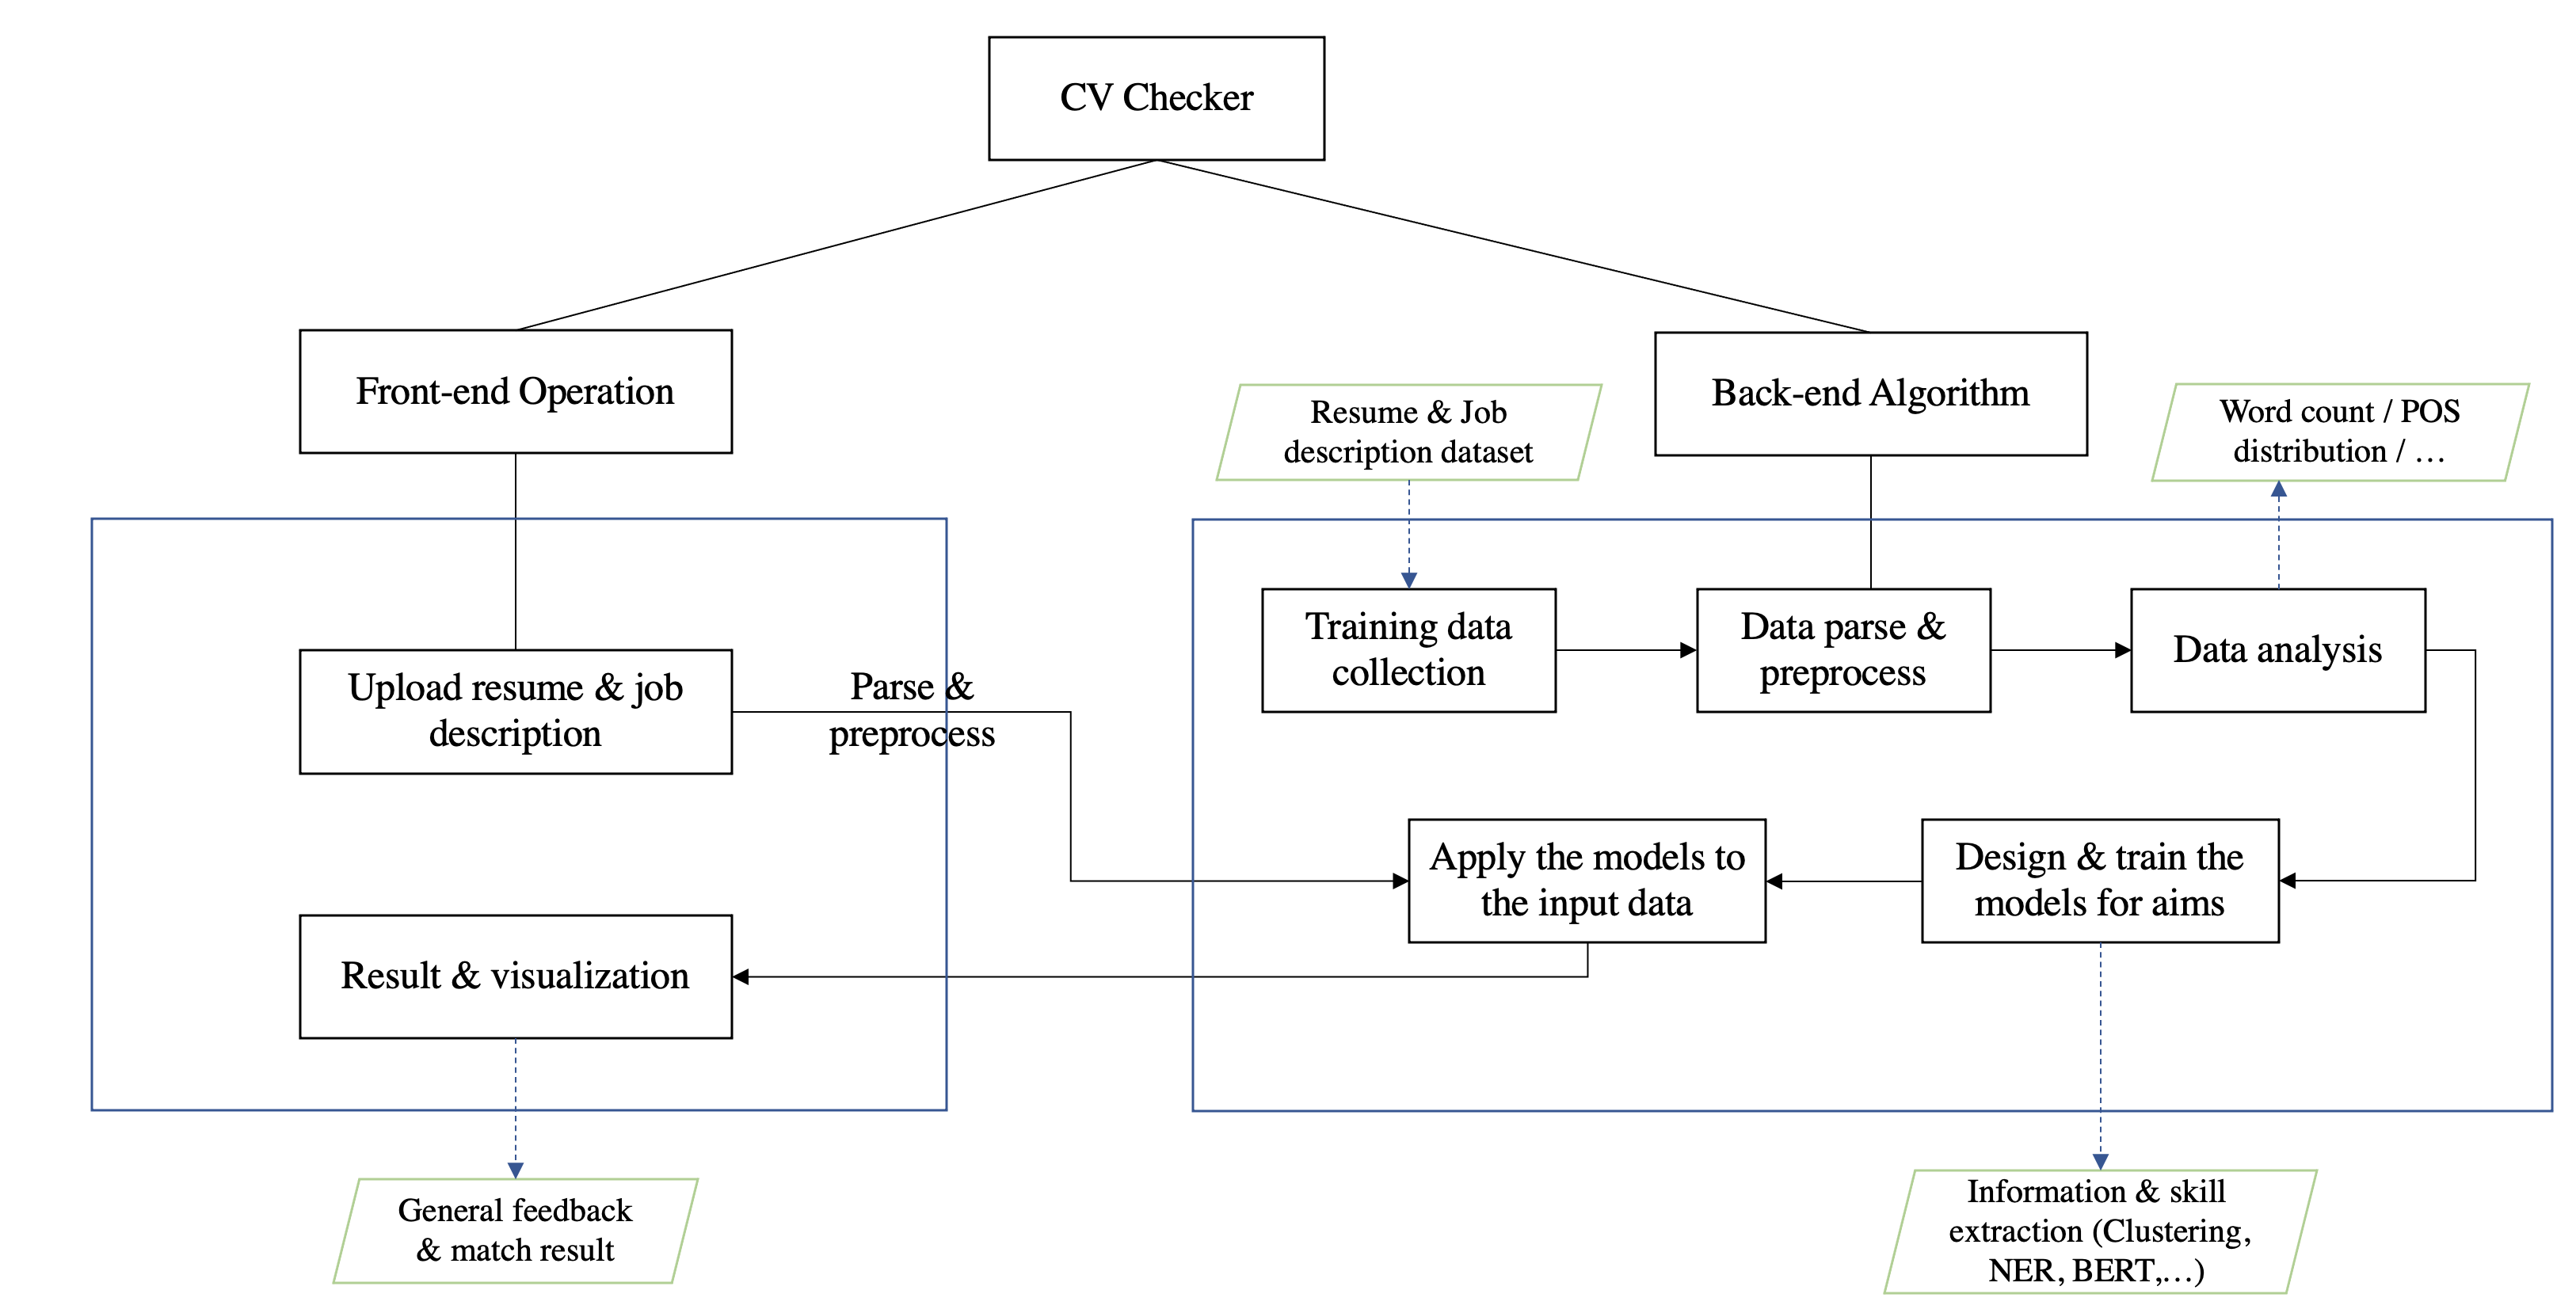
\includegraphics[width=1.2\textwidth]{images/overall_design.png}
    \caption{Overall Design}
    \label{fig:14}
\end{figure}




\section{Unified Modeling Language (UML)}

The Unified Modeling Language (UML) is a standard modeling language aiming on visualizing the design components of a software system \cite{siau2001unified}. UML includes structure diagrams and behaviour diagrams two basic types of diagrams , where structure diagrams are used to show the architecture of the system and behaviour diagrams are widely used to describe the functionalities of the system. In this section, two behaviour diagrams of this project, the sequence diagram and use case diagram, will be illustrated to represent the dynamic behaviour and functionality.

Sequence diagram depicts interactions between objects, focusing on lifelines and the message exchange between the processes. Since the interactions between the front-end and back-end in this project simply consist of uploading the resume file and the job description text data, and returning the feedback and matching result, the sequence diagram for this CV-checking website should be uncomplicated as shown in Figure \ref{fig:19}.


 \begin{figure}[H]
    \centering
    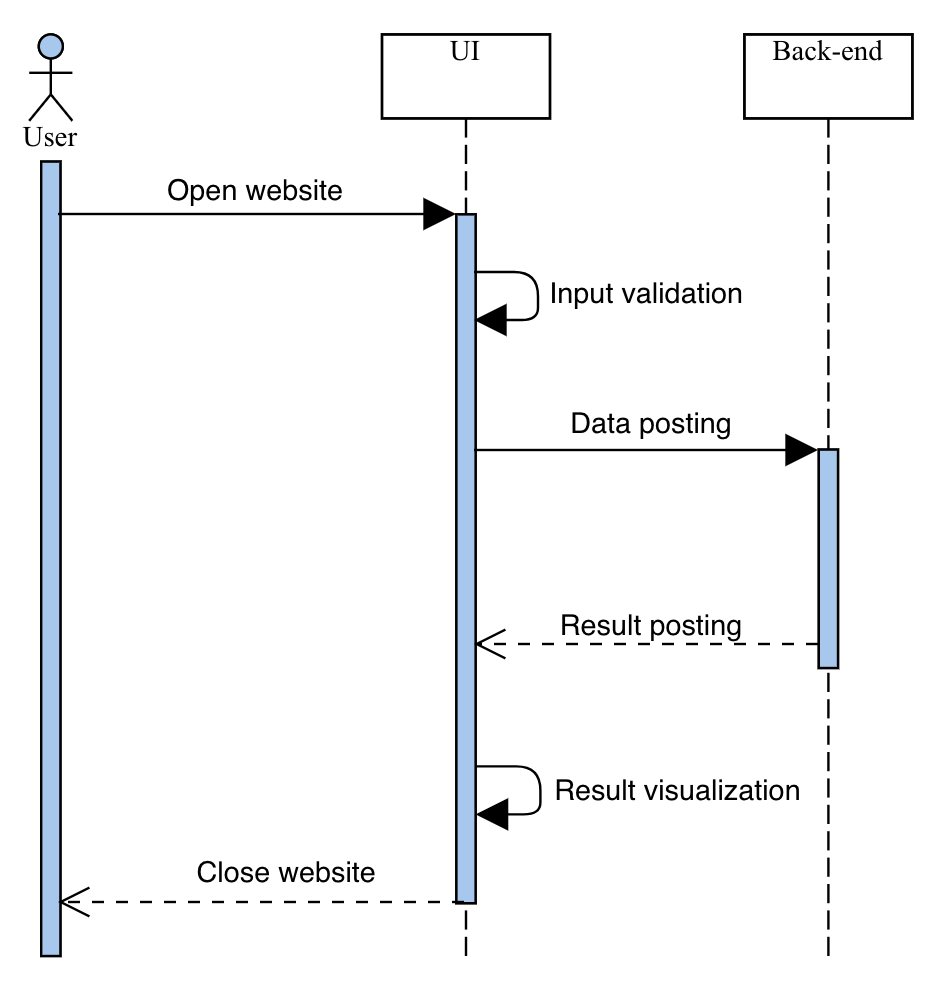
\includegraphics[width=0.6\textwidth]{images/sequence_diagram.png}
    \caption{Sequence Diagram}
    \label{fig:19}
\end{figure}

Use case diagram is also a behaviour diagram, which shows the interaction details between the actors and the system. Users and trained back-end models are regarded as the actors for our system, and the interactions are illustrated in the following Figure \ref{fig:20}.


 \begin{figure}[H]
    \centering
    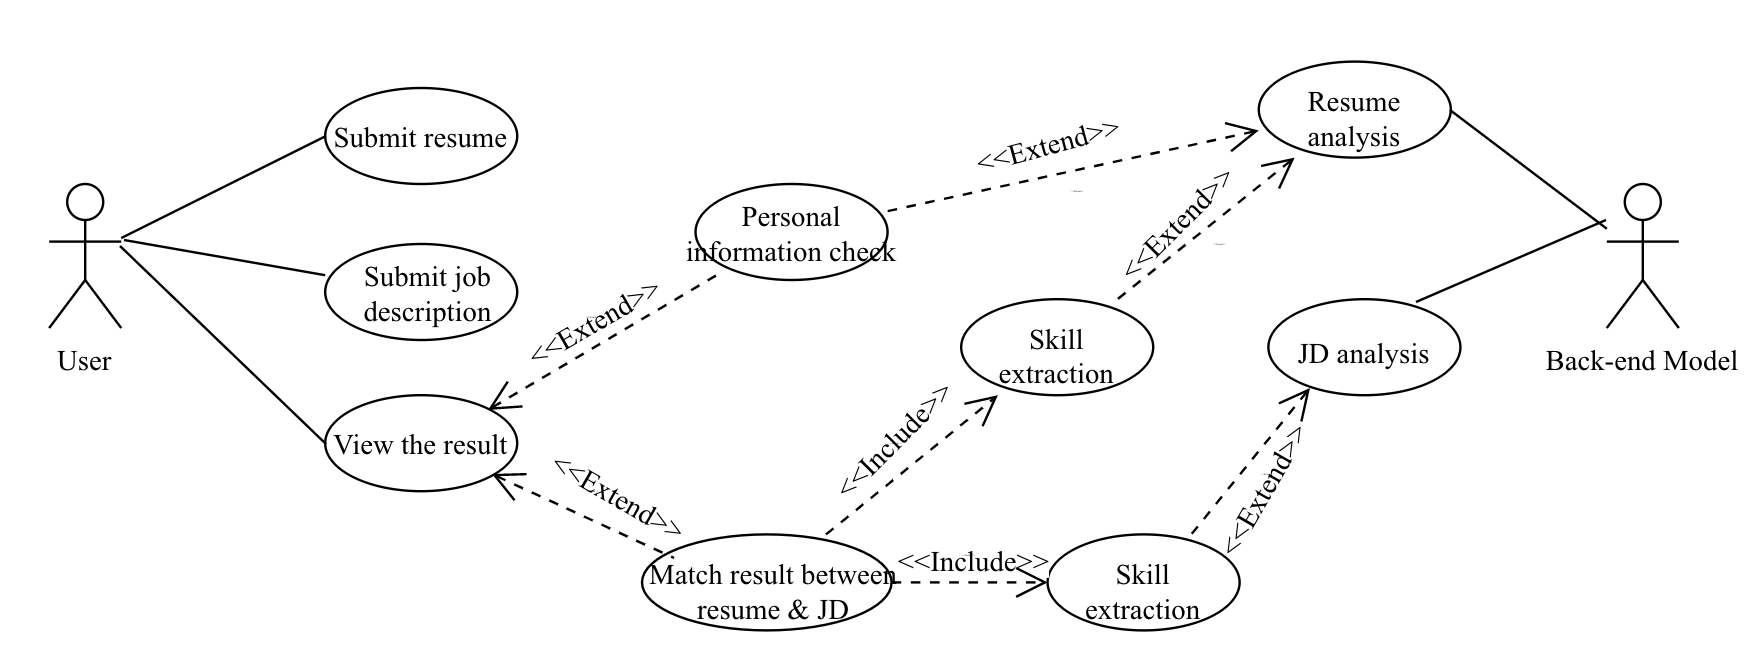
\includegraphics[width=0.9\textwidth]{images/usecase_diagram.png}
    \caption{Use Case Diagram}
    \label{fig:20}
\end{figure}


\section{User Interface}

User Interface (UI) is not set as a key objective of this project, but it still is an essential part of web development. The UI design for this project should consider the following requirements:

\begin{enumerate}
    \item The interface should be simple and straightforward.
    
    \item The website should allow users to choose a resume file and submit it. 
    
    \item The website should allow users to enter and submit the job description text.
    
    \item There should be some instructions for users to understand the usage of this application. For instance, it should be clarified which kinds of file formats could be submitted.
\end{enumerate}


 \begin{figure}[H]
    \centering
    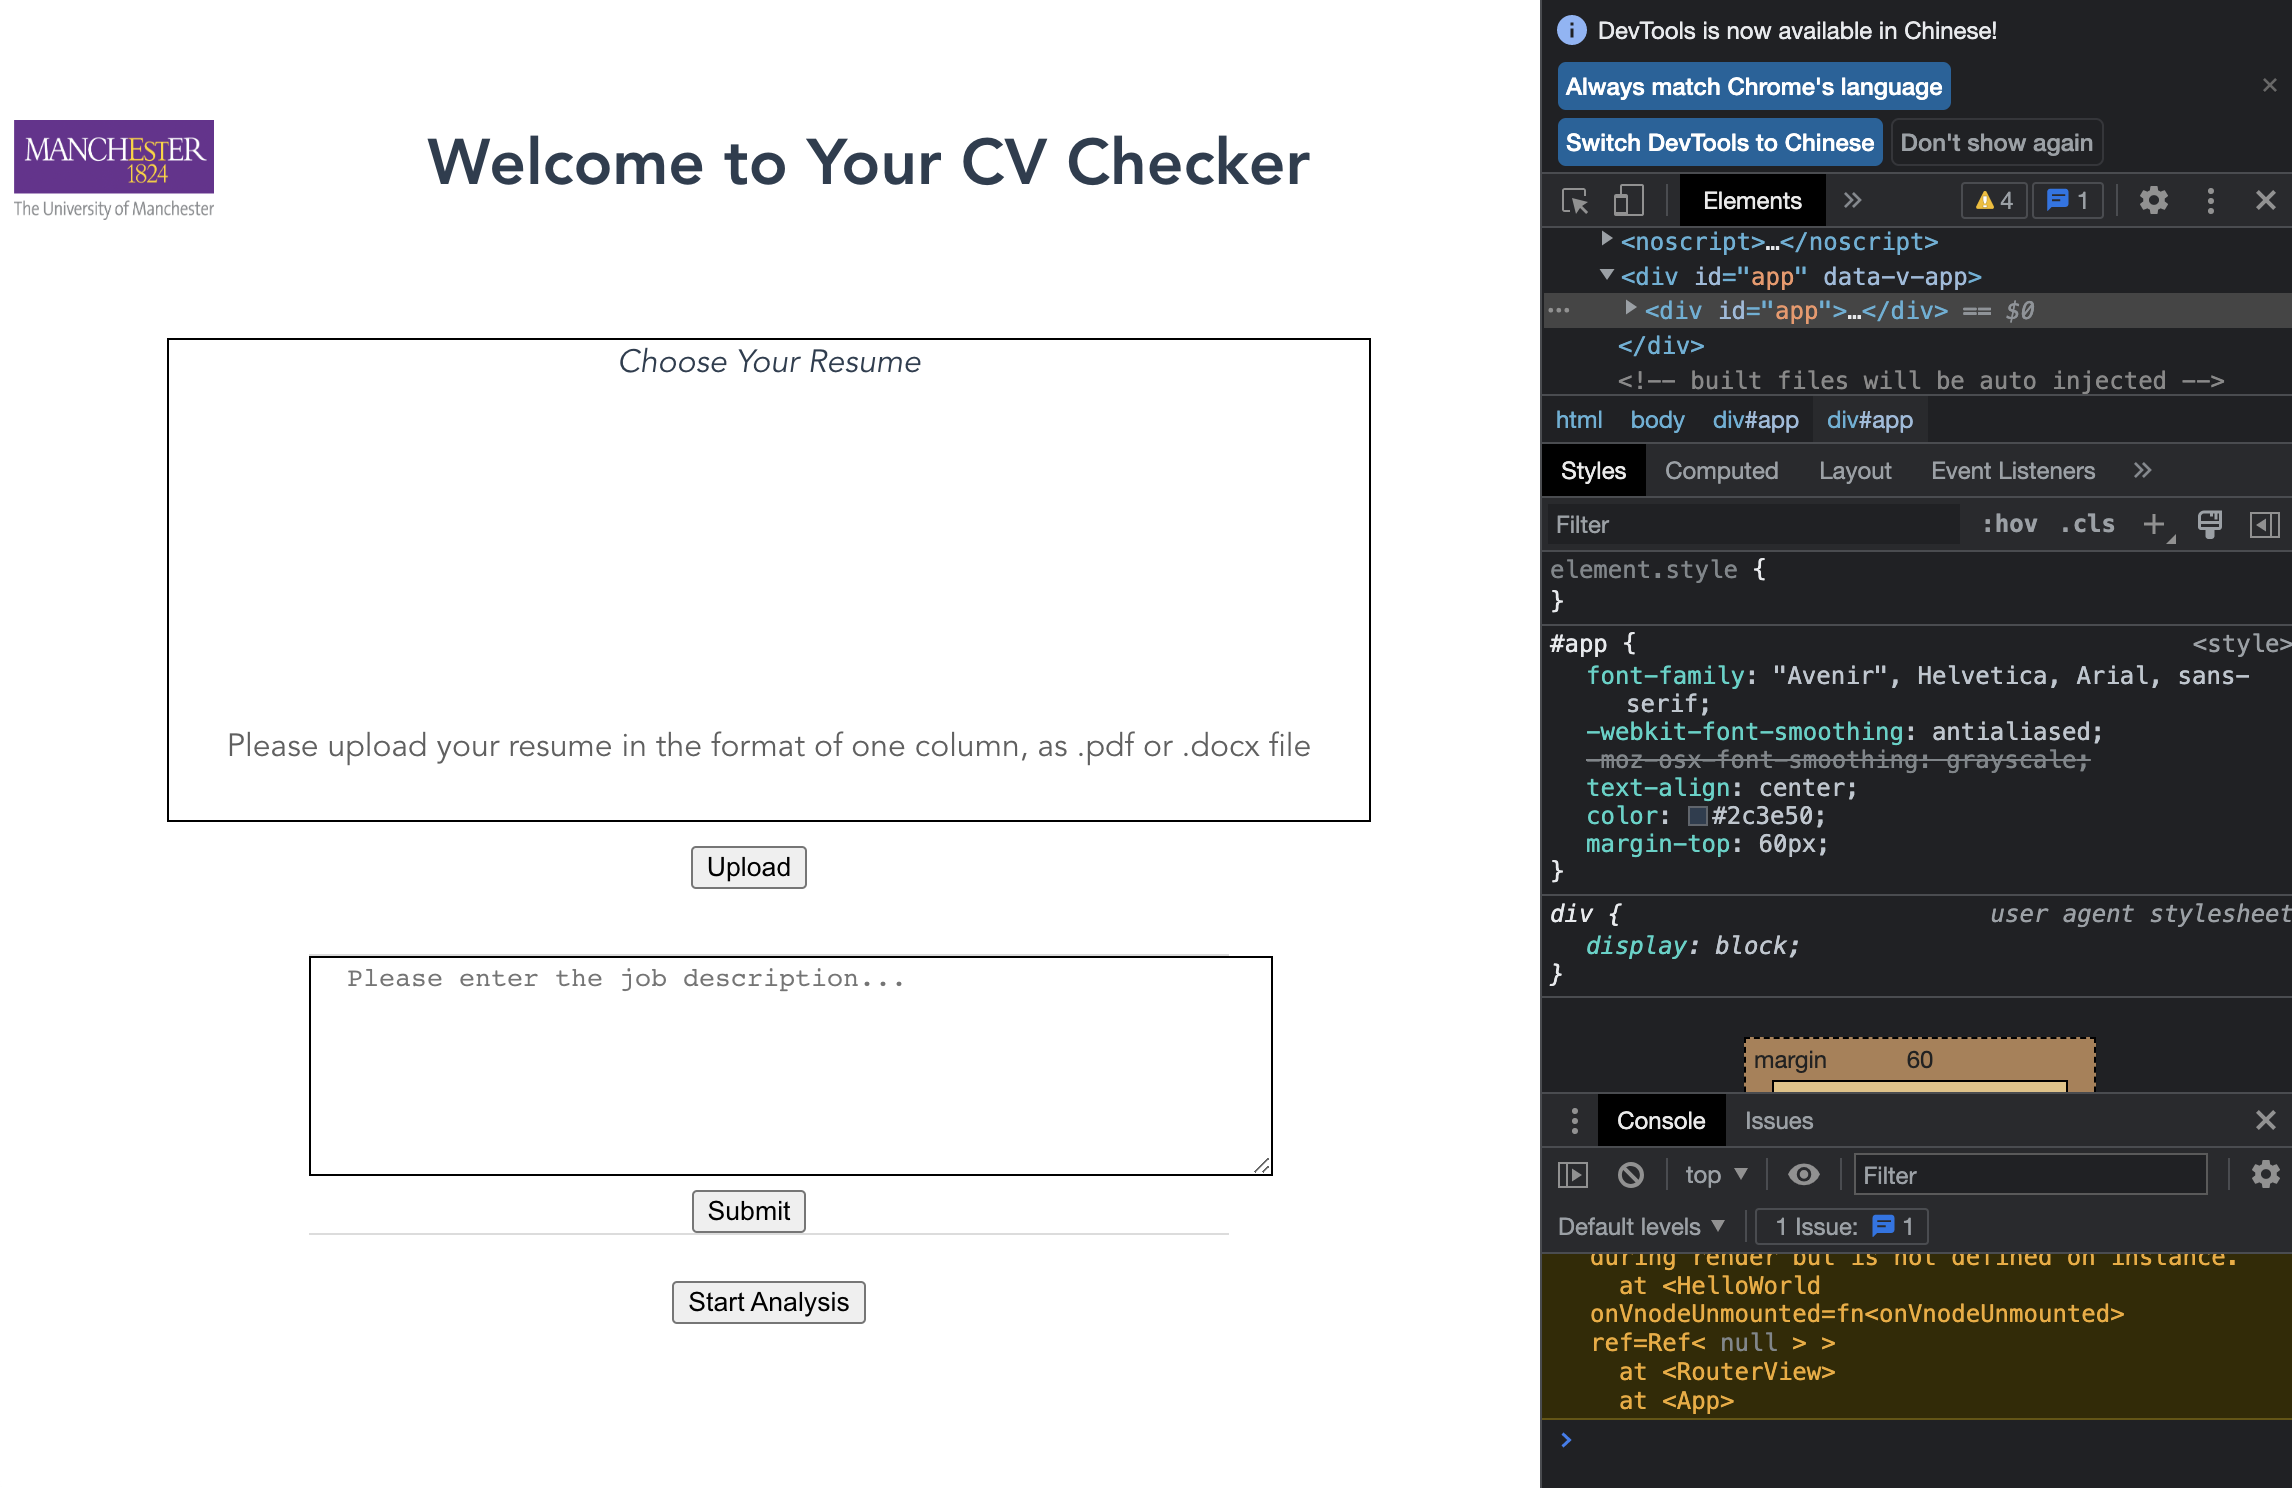
\includegraphics[width=1.2\textwidth]{images/ui.png}
    \caption{User Interface}
    \label{fig:35}
\end{figure}

Based on the design ideas, the above Figure \ref{fig:35} shows the simple user interface of the main page with the console. The top rectangle is for resume choosing and uploading, while the user can write the target job description in the bottom rectangle and submit the text. When submitting and uploading successfully, alerts would be returned on the screen. Then, the user can get the result page by pressing the 'Start Analysis' button.


\section{Data Preparation}

As illustrated in the previous section \ref{overall_design}, the resume and job description dataset should be collected for the back-end models training to implement the key information and skill extraction tasks from the input resume and job description text. This section will introduce the data preparation of the project in two parts; one is data collection, followed by the preprocessing steps for the training data in detail.

\subsection{Data Collection}
\label{sec:data}

To obtain the training data, the following requirements should be taken into consideration:

\begin{enumerate}
    \item Both resume and job description dataset should be large enough to learn the features.
    \item The resume dataset should be annotated with named entities for SpaCy NER model training, containing at least person name, e-mail address, educational information and skills , which means the label should in a specific format to point the named entities and their locations (start and end) in the data.
    \item The job description dataset is expected to cover sufficient positions from different area.
\end{enumerate}

Kaggle, a platform for data science and machine learning researchers, provides plenty of open-sourced datasets, notebooks and projects. The job description dataset used in this project is acquired from Kaggle, which contains 19,000 job postings from 2004-2015 with the content of job title, company, location, job description, job requirement, et cetera. This dataset can be accessed on \href{https://www.kaggle.com/datasets/madhab/jobposts?datasetId=1150}{Kaggle}, and has been used in multiple related tasks for job description analysis.

The resume dataset with named entities annotations is collected from an open-sourced similar project, which can be accessed on \href{https://github.com/OmkarPathak/pyresparser}{Github}. This dataset consists of 700 labeled resumes, where personal profile named entities like name, email, mobile numbers, and the entities of other information such as skills, experience, and college name are all located and annotated for NER model training.

Additionally, there is another published dataset containing multiple real-word resumes with both .pdf and .doc file format, which is available on \href{https://github.com/Msq-9/Extraction-of-Skills}{Github}. These resumes can be utilized to test our CV-checking application as the user input.

\subsection{Data Preprocessing}

Data preprocessing is a significant and essential step before applying the data to machine learning algorithms. Especially for text data, there are many structural variations of terms in the natural language and the structure of text data could be complex and inconstant \cite{kannan2014preprocessing}, which makes the preprocessing phase necessary for the tasks involving text data. The primary aims of data preprocessing is to reduce the noises, preserve the features of the text, and obtain clean and normalized data. To achieve the above goal of preprocessing, the graphical design of preprocessing pipeline is as follows in Figure \ref{fig:15}.

 \begin{figure}[H]
    \centering
    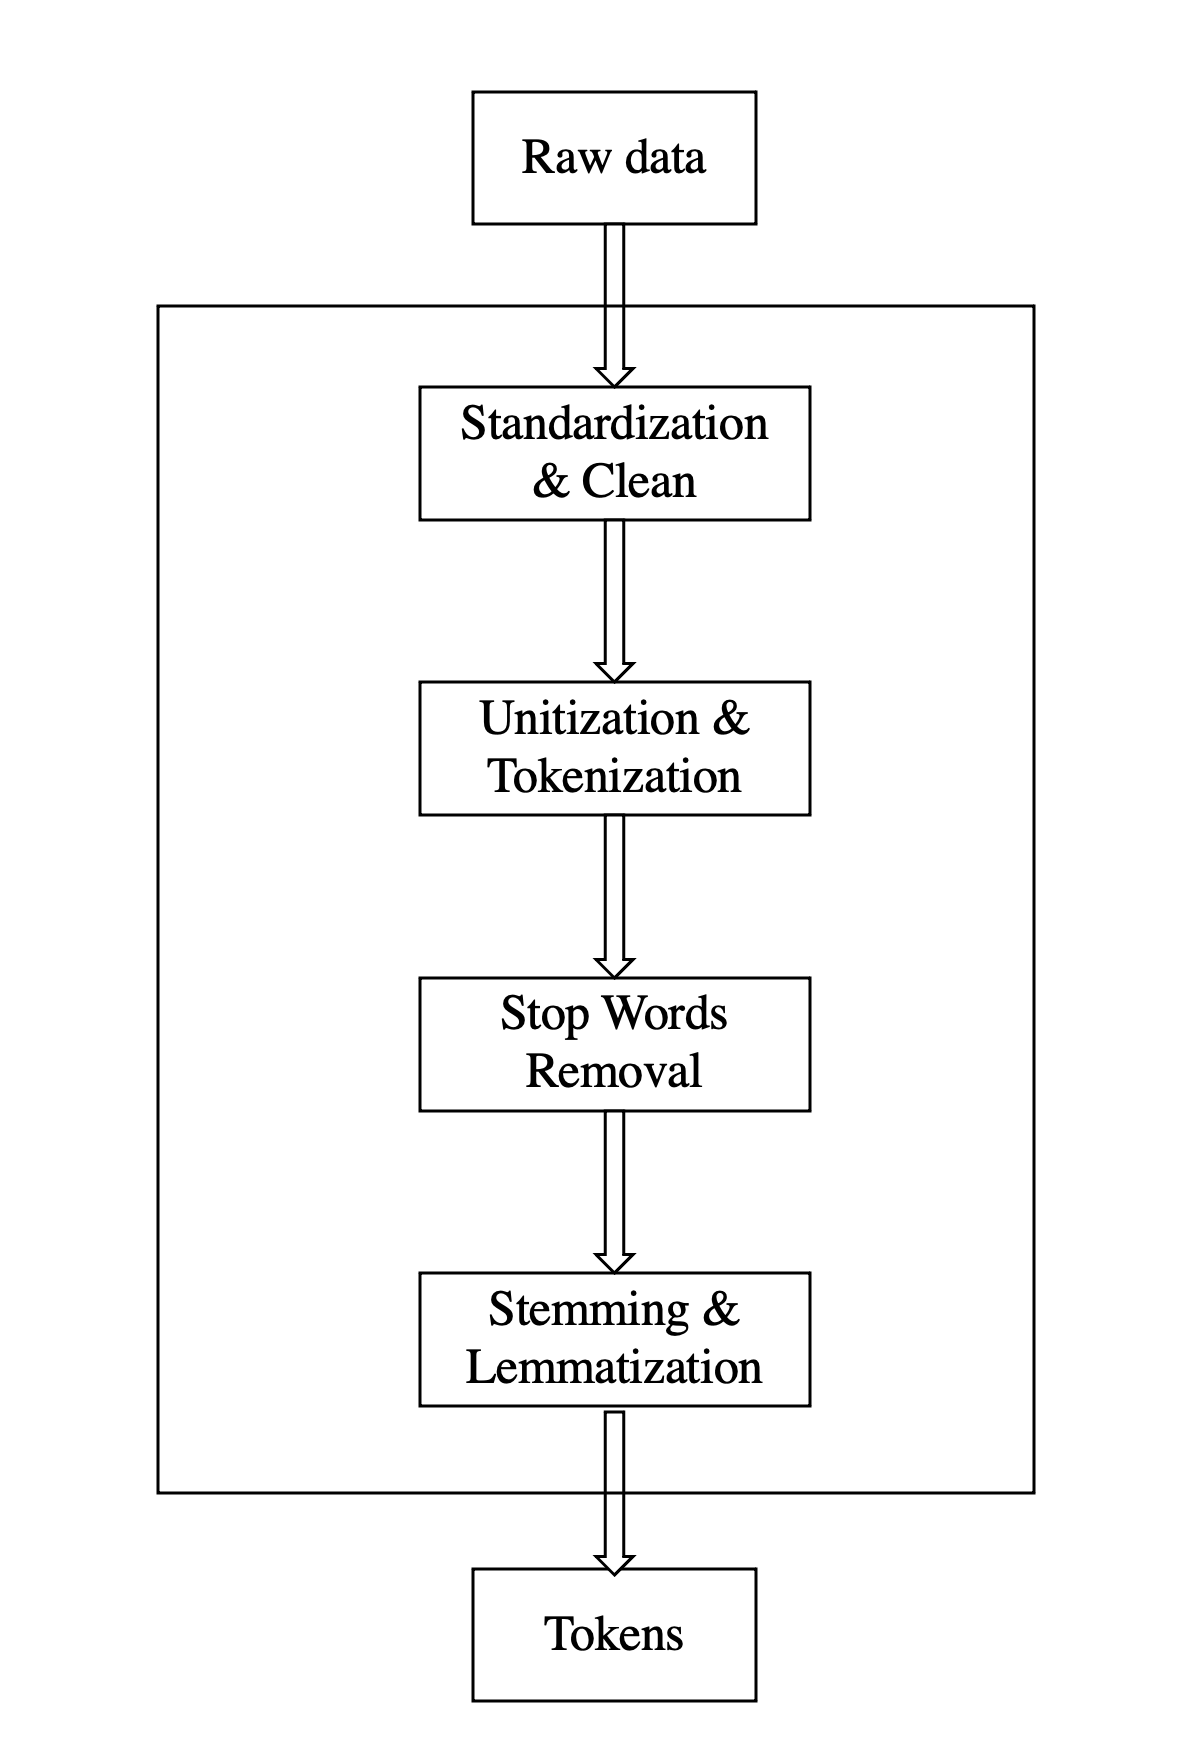
\includegraphics[width=0.45\textwidth]{images/preprocessing.png}
    \caption{Preprocessing Pipeline}
    \label{fig:15}
\end{figure}

The main steps of data preprocessing include: 1) standardizing and cleaning the data by removing punctuation, special characters and format using regular expressions, 2) unitization and tokenization to get smaller units from the document to understand the data structure, in terms of sentence tokens and word tokens, then lower case all the tokens, 3) removing the stop words such as pronouns and preposition by NLTK stop words list, 4) stemming and lemmatization, then tagging with POS. As introduced in Section \ref{method_preprocessing}, NLTK is used as the tool for the above preprocessing processes. Moreover, after preprocessing the data, visualization techniques such as word cloud and histogram will be used for data analysis to show the keywords and word distribution. The examples of the visualization result are as follows. Through manual check, the related words computed by word vectors are reasonable, which means this word2vec model performs well.

\begin{figure}[H]
    \begin{minipage}[t]{0.5\linewidth}
        \centering
        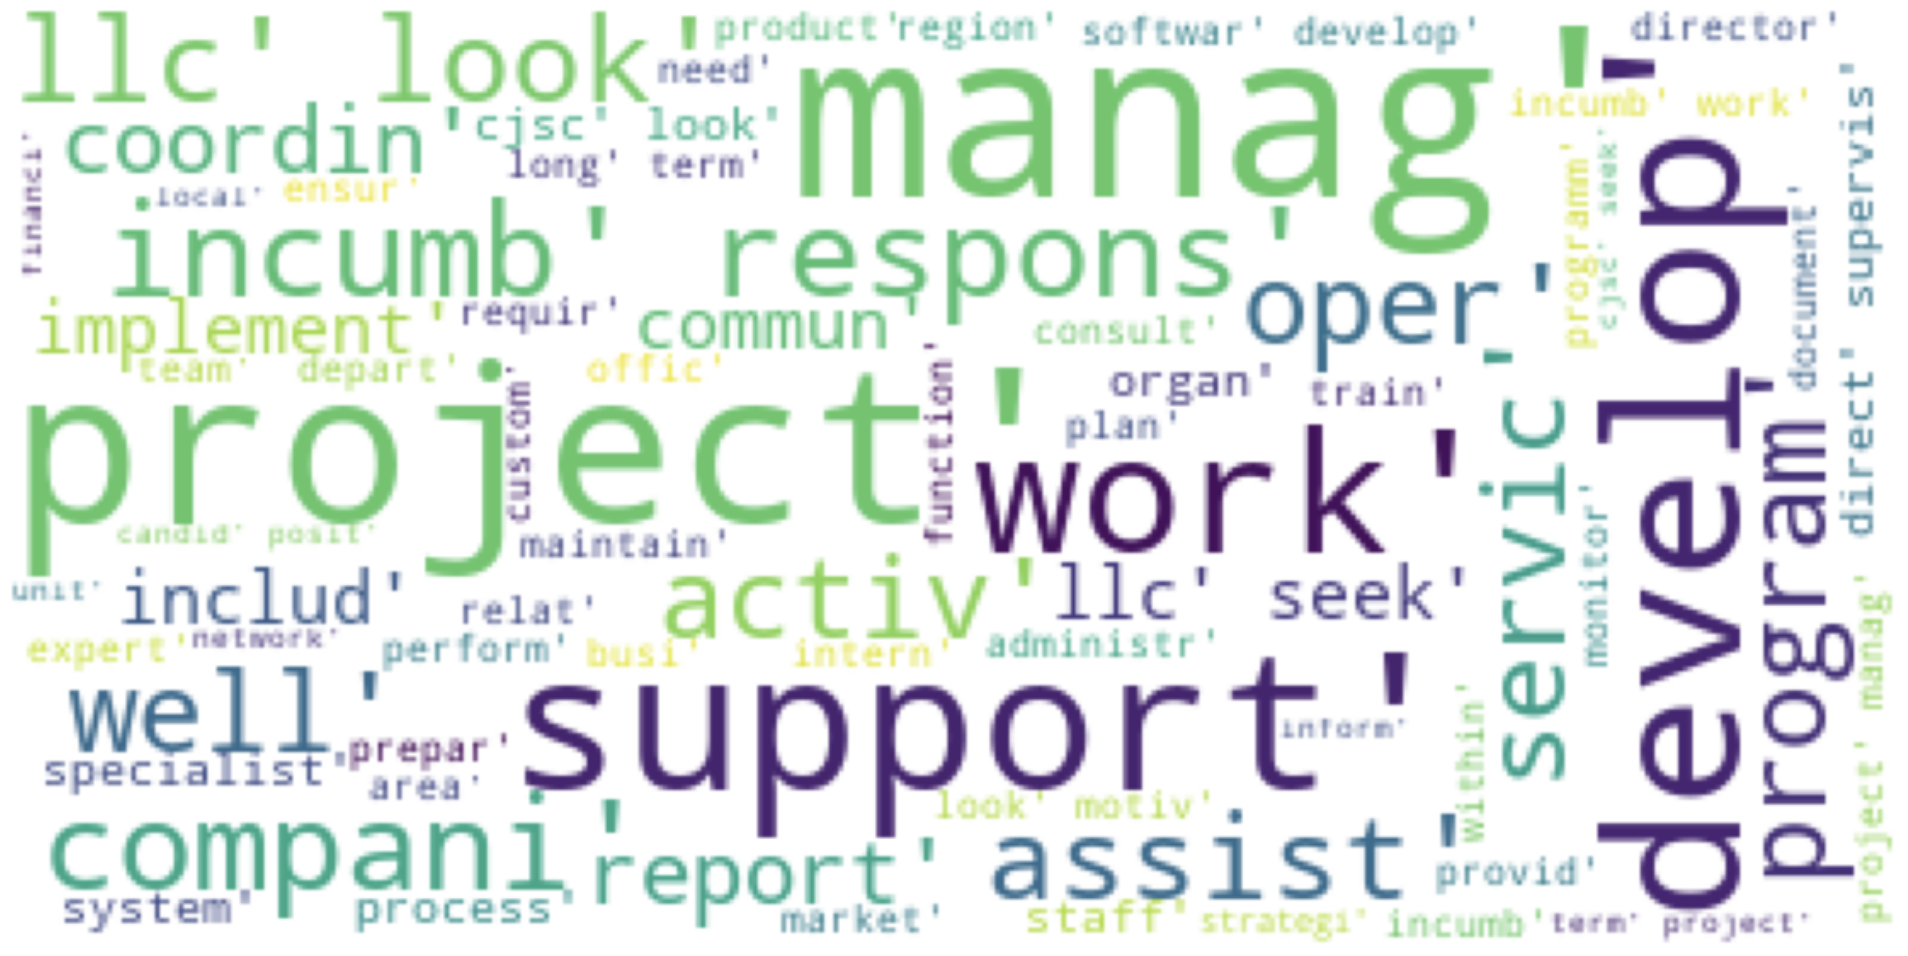
\includegraphics[scale=0.2]{images/wordcloud_exp.png}
        % \caption{Word Cloud}
        \label{fig:16}
    \end{minipage}%
    \begin{minipage}[t]{0.5\linewidth}
        \centering
        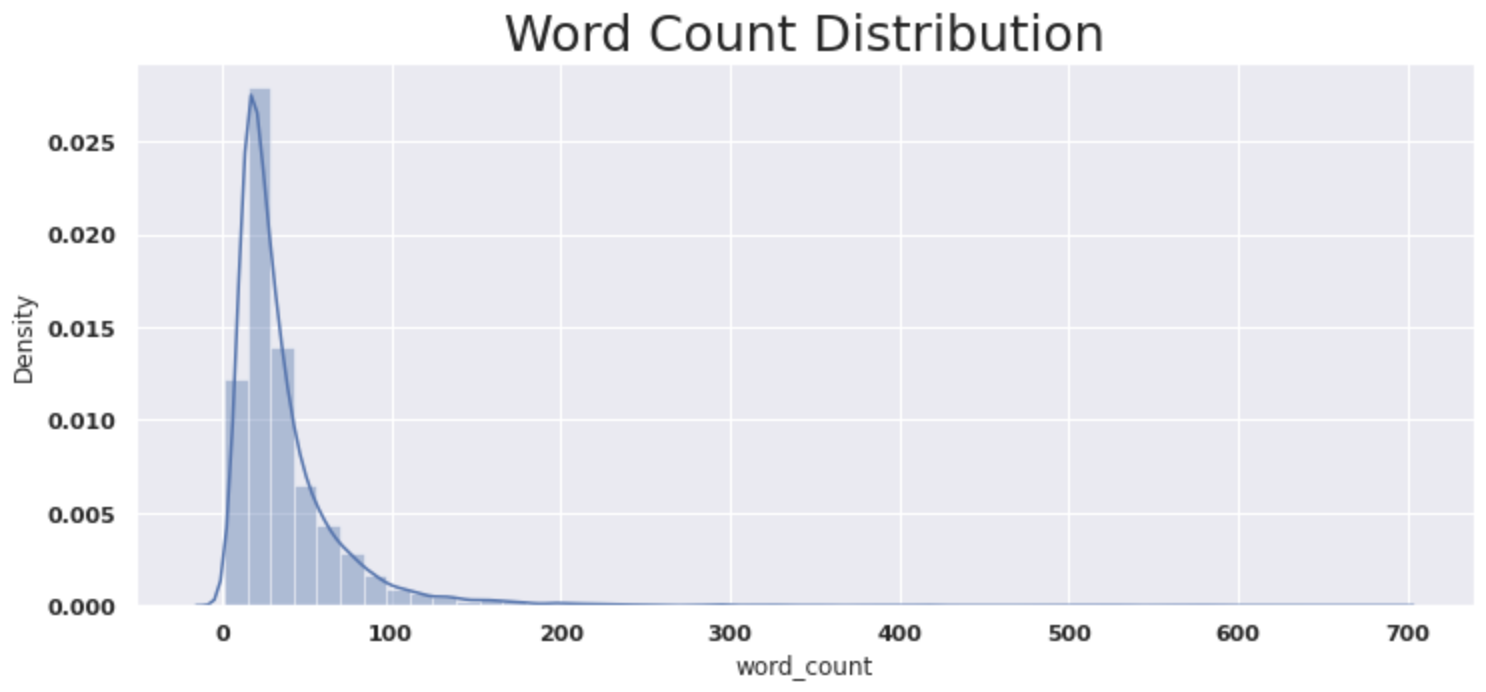
\includegraphics[scale=0.3]{images/distribution_exp.png}
        % \caption{Histogram}
        \label{fig:17}
    \end{minipage}
    \caption{Example of Visualization}
\end{figure}

By using the word vectors as the training samples, K-means algorithm could be applied to get the clusters. 

\section{Back-end Algorithms}
\label{sec:backend_design}

With the preprocessed training data, back-end algorithms are designed to recognize key information, extract skills and compute the match rate tasks like the existing CV checkers such as \href{https://www.jobscan.co/}{Jobscan}. The following specifications should be considered when designing models:

\begin{enumerate}
    \item The system should be able to understand the content of the submitted new resume and check the coverage of basic information such as person name, email address, educational detail, etc.
    
    \item The system should be able to extract the skills mentioned in the submitted resume.
    
    \item The system should be able to discover the requirements of the position from the job description by skill extraction.
    
    \item The system should enable to match the person's skills and the position requirements, and return the match rate combined with detailed result.
\end{enumerate}

 \begin{figure}[H]
    \centering
    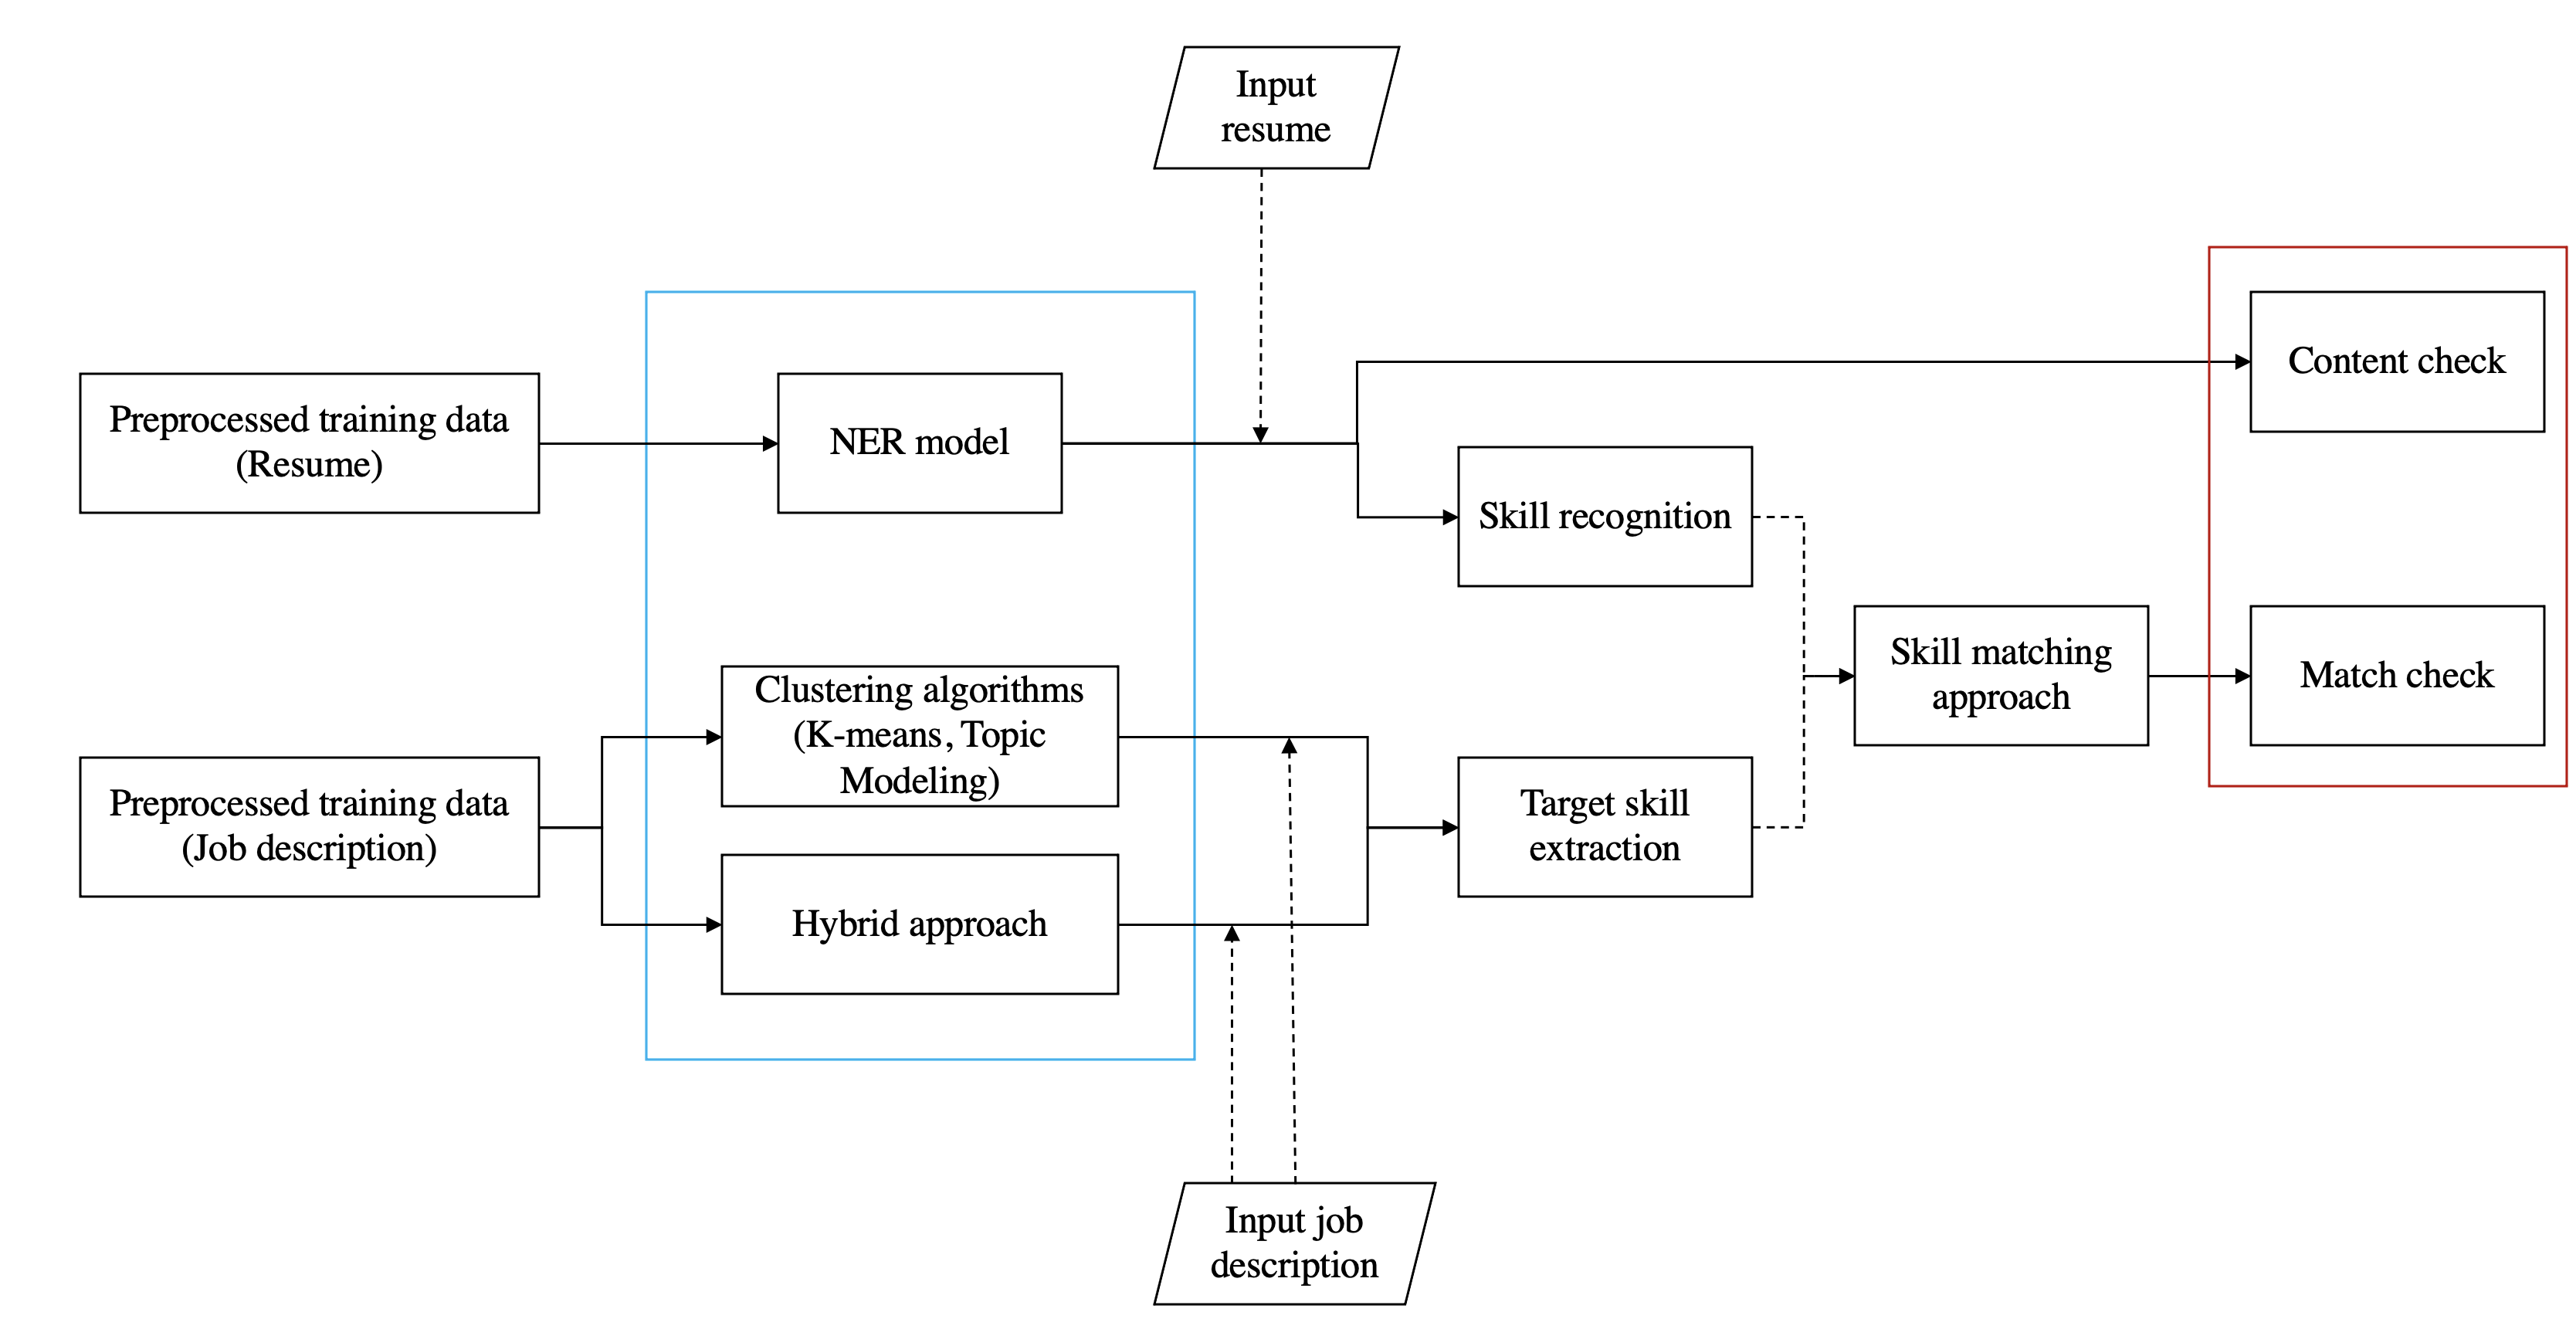
\includegraphics[width=1.2\textwidth]{images/backend_design.png}
    \caption{Back-end System Design}
    \label{fig:18}
\end{figure}

In order to fulfill the specifications, the general design of the back-end system is presented in the above diagram \ref{fig:18}. Because the inside algorithms of the existing CV checkers could not be known to the public, though the functionalities of our project refer to the existing CV checker, the implementation of the functionalities is like a black box for us. In this case, various approaches, which have been described in Chapter \ref{ch:methodology}, need to be experimented during the development to find a suitable approach for target tasks. In the diagram of the back-end design, the blue area refers to the experimented models and approaches to implement different functionalities, the dashed arrows denote applying the input data to the trained models for prediction or extraction, and the red area means the two final targets. As for the aim of the content check, preprocessed resume data is used to train an NER model, which will be applied to the input resume to check the coverage of the necessary information. Since the training dataset contains the skill annotation as well, the NER model could also be used to recognize the skills from the input resume. For the target of the match check, besides skill extraction from the input resume, the skills in the uploaded job description should also be identified. The preprocessed job description dataset should be used as the training set, and experiments on different approaches are needed for the extraction task. With the extracted skills from the input resume and job description, the skill matching approach can be used for the match check.

Chapter \ref{ch:methodology} introduced several libraries to train the models for the CV checker. NER model training for the content check is implemented by spaCy, K-means clustering training is provided by Scikit-learn, and LDA topic model can be achieved by Gensim. 

As for the hybrid approach for determining skills in the job description, the basic processes have been shown in section \ref{sec:hybrid}. After tagging the POS of tokens by NLTK, regular expression chunking techniques should be used to obtain reasonable chunks. According to \cite{ketterer}, skills usually appear in four kinds of patterns, and their regular expressions are described as follows:

\begin{enumerate}
    \item Basic Noun Phrase: including singular and plural noun, proper noun, noun with a determinate, and noun with adjectives. The regular expression can be written as $\{<DT>?<JJ>*<NN|NNS|NNP>+\}$, where $"?"$ means optional included, $"*"$ refers to any number of tags included and $+$ means including one or more. $DT$ is the POS tag for determiner, $JJ$ means adjective, $NN$, $NNS$, $NNP$ are singular noun, plural noun and proper noun separately.
    
    \item Variation of Noun Phrase: containing an optional preposition or conjunction, followed by nouns or adjectives and ending with a singular noun or plural noun. Its regular expression is $\{<IN>?<JJ|NN>*<NNS|NN>\}$, where $IN$ is the POS tag for preposition.
    
    \item Verb Phrase: including all kinds of verbs followed by a singular noun or plural noun. The regular expression is $<VBG|VBZ|VBP|VBD|VB|VBN><NNS|NN>*$
    
    \item Nouns splitted by comma: this situation is considered because some of the job descriptions might list the expected requirements (skills) separated by comma. The regular expression could be $<NN|NNS>*<,><NN|NNS>*<,><NN|NNS>*$
    
\end{enumerate}

After defining the regular expressions of the patterns, NLTK RegexChunkParser can find the chunks in the text by using those regular expressions as the rules. Manually labeling the chunks, the training dataset is prepared. The subsequent neural network with BERT layer is built based on Keras, an API for high-level neural networks running on top of the TensorFlow machine learning platform \cite{keras}. The architecture of the deep learning neural network with BERT layer is shown in the following Figure \ref{fig:12}.

 \begin{figure}[H]
    \centering
    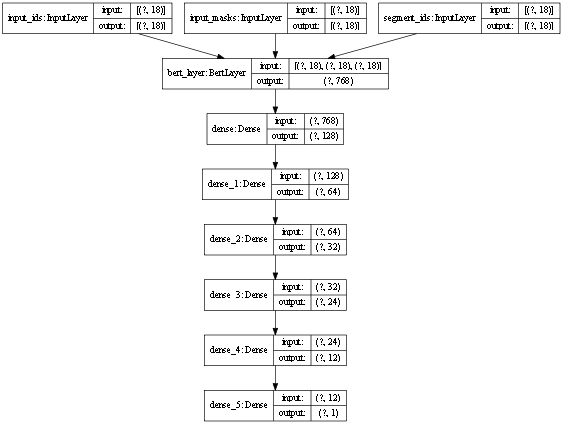
\includegraphics[width=0.9\textwidth]{images/withBERT.png}
    \caption{Architecture of Neural Network \cite{ketterer2}}
    \label{fig:12}
\end{figure}

With the extracted skills from the resume and the job description, the match rate can be obtained by calculating the cosine similarity from the text.
% skill matching implementation

% \section{Visualization Result}


\chapter{Result \& Evaluation}
% \addcontentsline{toc}{chapter}{Evaluation}
\label{ch:evaluation}

This chapter will provide the evaluation of the application via the experimental results and the overall visualization result. 

\section{Evaluation Method}

In order to evaluate the back-end machine learning approaches such as NER and deep learning models, accuracy, precision and F1 score can be used to examine the quality of the output result. Due to the human-readable characteristic of natural language, the feedback returned from the CV checker could be checked manually. Moreover, comparing with the result of existing systems and applications could also help to evaluate the performance of our application.


\section{Experimental Result}
Experimental results contain the results and evaluations for both dataset and all experimented back-end AI algorithms, including information extraction by NER, skill extraction and skill match.

\subsection{Information Extraction Result}
\label{sec:ner_result}

With the annotated resume dataset, which has been introduced in Section \ref{sec:data}, an NER model is trained for the information extraction task to check the CV content. The dataset is divided into the training set and test set with the ratio of 9:1. $Scorer.score$ module provided by spaCy is used to evaluate the NER model, which can calculate the precision, recall and f1 score of the model for each entity and the average score for all entities as well. The following table shows the evaluation result of our NER model, with the average score for all entities and the scores for some important entities. 


\begin{table}[htbp]
\centering
\begin{tabular}{|c|c|c|c|}
\hline
Entity Type & Precision & Recall & F1 Score\\
\hline
Name & 0.94 & 0.99 & 0.96\\
\hline
Designation & 0.58 & 0.72 & 0.65\\
\hline
Companies worked at & 0.72 & 0.77 & 0.74\\
\hline
Email Address & 0.94 & 0.95 & 0.95\\
\hline
Degree & 0.71 & 0.86 & 0.78\\
\hline
Skills & 0.50 & 0.35 & 0.41\\
\hline
Average & 0.63 & 0.57 & 0.60\\
\hline
\end{tabular}
\caption{Result of NER Model}
\label{tbl:4}
\end{table}

% too many types of entities, various of skill expressions, insufficient of training set

There are over fifteen types of named entities in the training set, some of which are not very common in resume data. In this case, the named entity labels in the training set are insufficient, and the obtained score of each entity are uneven. So, the average precision, recall and F1 score of all entities are not very high with about 0.60. By focusing on parts of results, the recognition results of the entities we are most concerned about are listed in the above Table \ref{tbl:4}. The obtaining scores for the basic information like Name and Email Address are pretty high with almost over 0.95, while the work experience recognition such as designation and companies are lower with around 0.70. As for the task of identifying skills in the resume, this NER model did not perform well though there are numerous annotations for skill entity. Through this result, it can be observed that recognition of the entities with similar patterns or expressions in different resumes such as Name and Email Address could get a high score. In contrast, the entities with diverse and complex expressions such as skills, obtained lower scores. Extending the training set could be one solution for getting a better result. According to \cite{fu2020interpretable}, the labeling consistency also affects the NER model, which could be regarded as the future work of our project.



\subsection{Data Analysis}

This section will give the visualization analysis of the job description dataset for skill extraction since visualization of the dataset can help the developer to have a deep understanding of the data for further processes. The job description dataset from Kaggle collected 19,001 job position details with 24 columns, including job title, company, job requirement, required qualification, etc. The column of job requirements is used in this project to obtain as many skills as possible.

After obtaining the tokens of the clean dataset by removing punctuation and special characters, the following figures show the word count and sentence count distribution of the job description (job requirement) text in the dataset, with a mean value of 95 words and eight sentences in each job description.

\begin{figure}[H]
    \begin{minipage}[t]{0.5\linewidth}
        \centering
        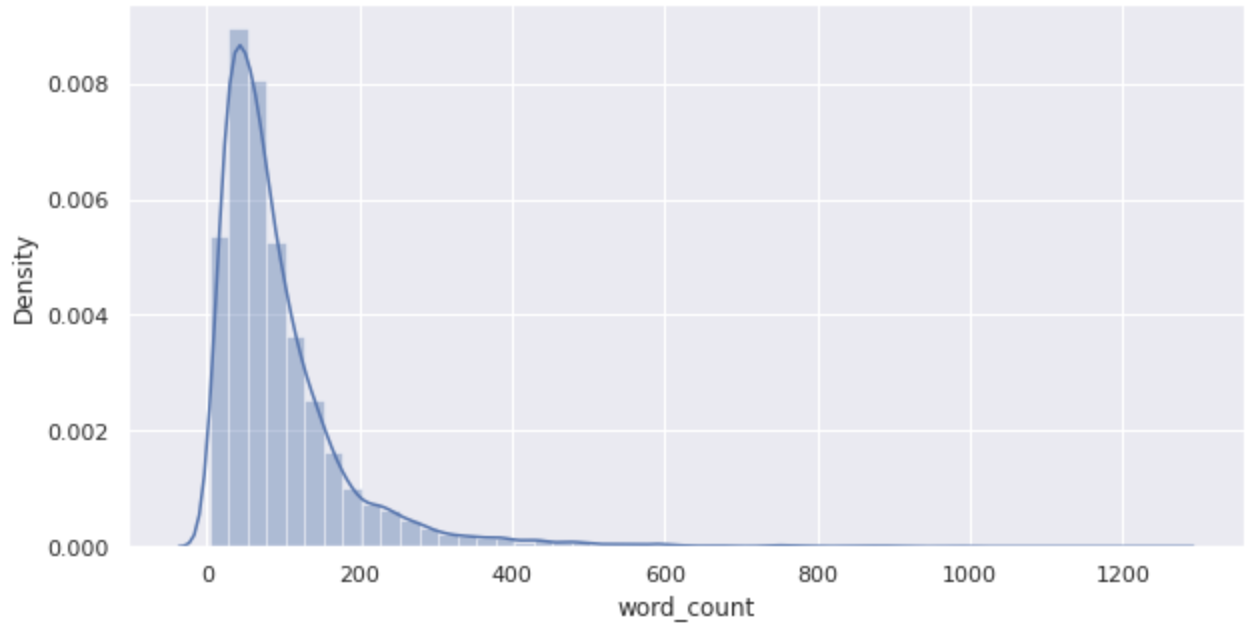
\includegraphics[scale=0.35]{images/wordcount.png}
        \caption{Word Distribution}
        \label{fig:21}
    \end{minipage}%
    \begin{minipage}[t]{0.5\linewidth}
        \centering
        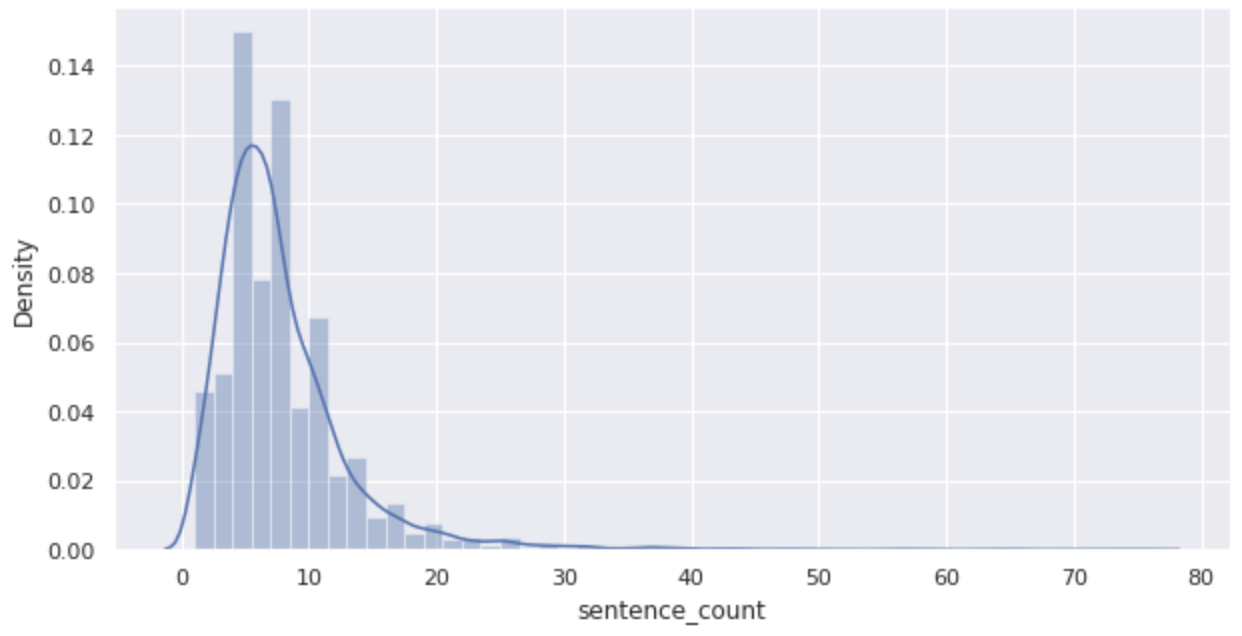
\includegraphics[scale=0.35]{images/sentencecount.png}
        \caption{Sentence Distribution}
        \label{fig:22}
    \end{minipage}
\end{figure}

With the preprocessing steps including stop words removal and lemmatization, the word frequency in the corpus is presented through histogram as Figure \ref{fig:23}. In order to see the words more straightforward, the most frequent words in the corpus are shown in Figure \ref{fig:24} via word cloud.

% \begin{figure}[H]
%     \centering
%     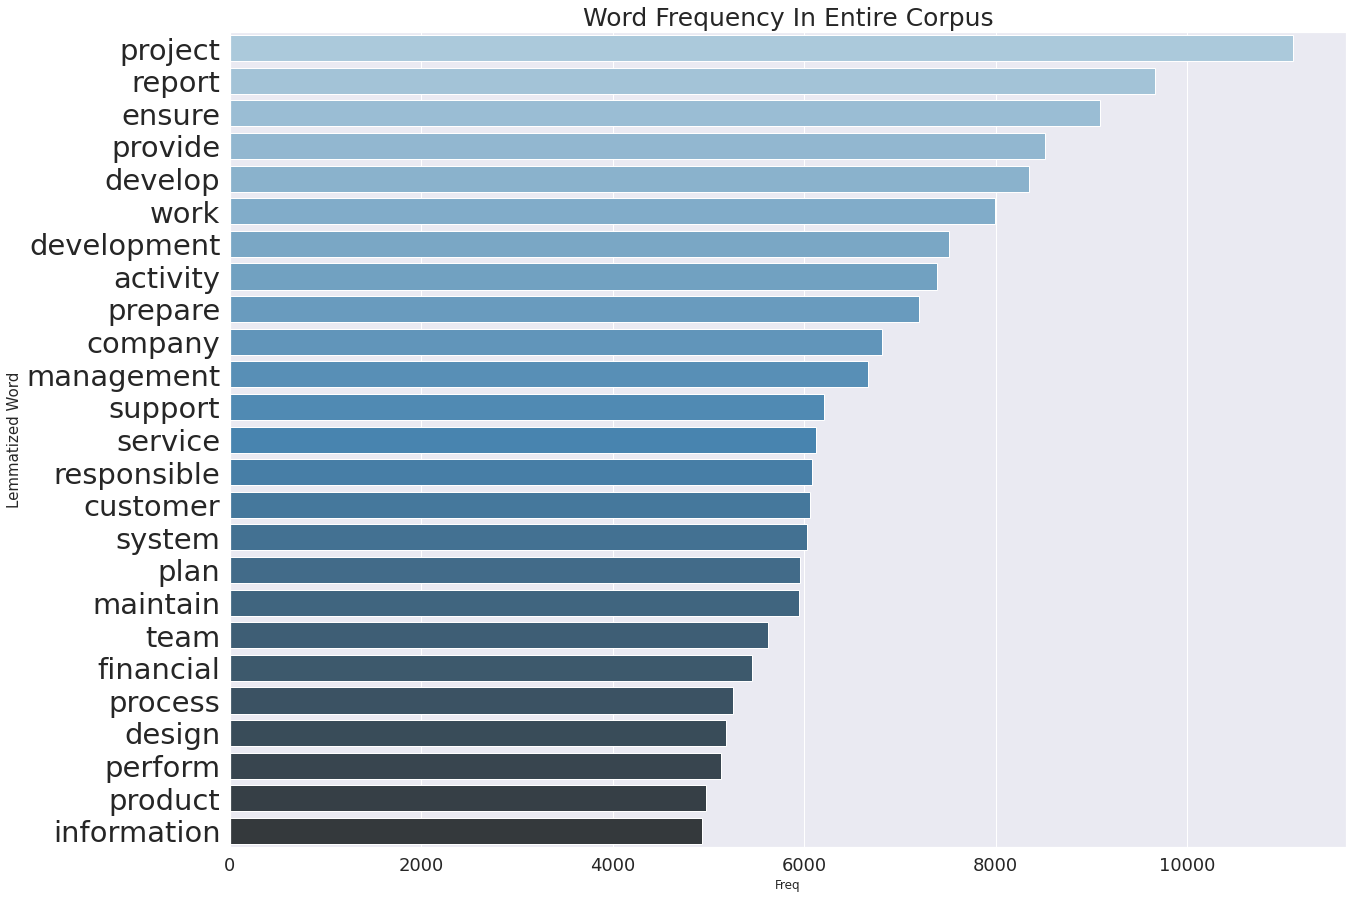
\includegraphics[width=0.7\textwidth]{images/frequent_hist.png}
%     \caption{Histogram of Word Frequency}
%     \label{fig:23}
% \end{figure}


% \begin{figure}[H]
%     \centering
%     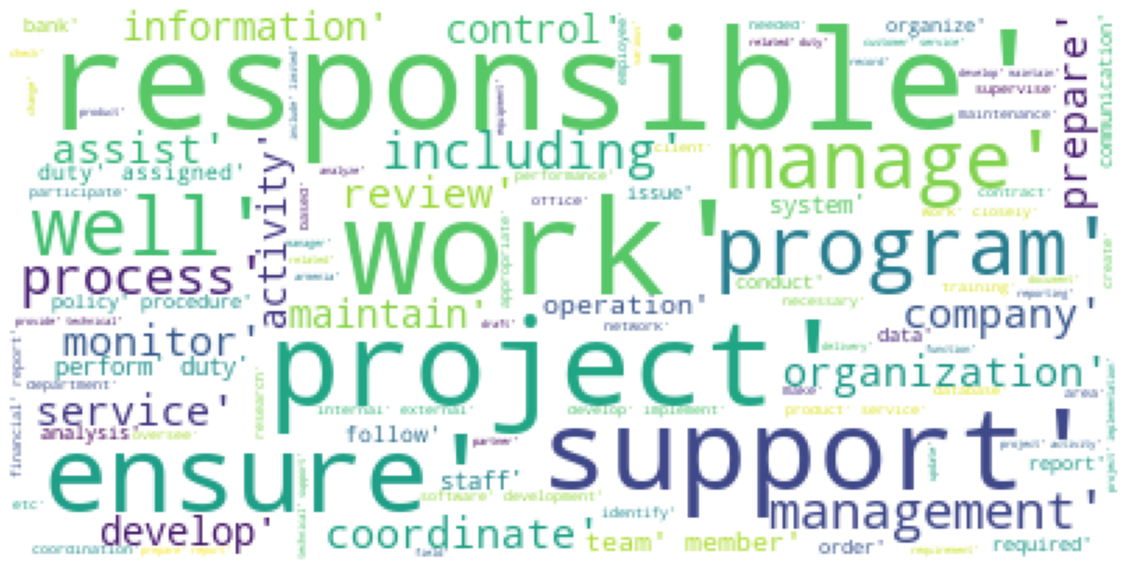
\includegraphics[width=0.6\textwidth]{images/frequent_cloud.png}
%     \caption{Word Cloud for Frequent Words}
%     \label{fig:24}
% \end{figure}

\begin{figure}[H]
    \begin{minipage}[t]{0.5\linewidth}
        \centering
        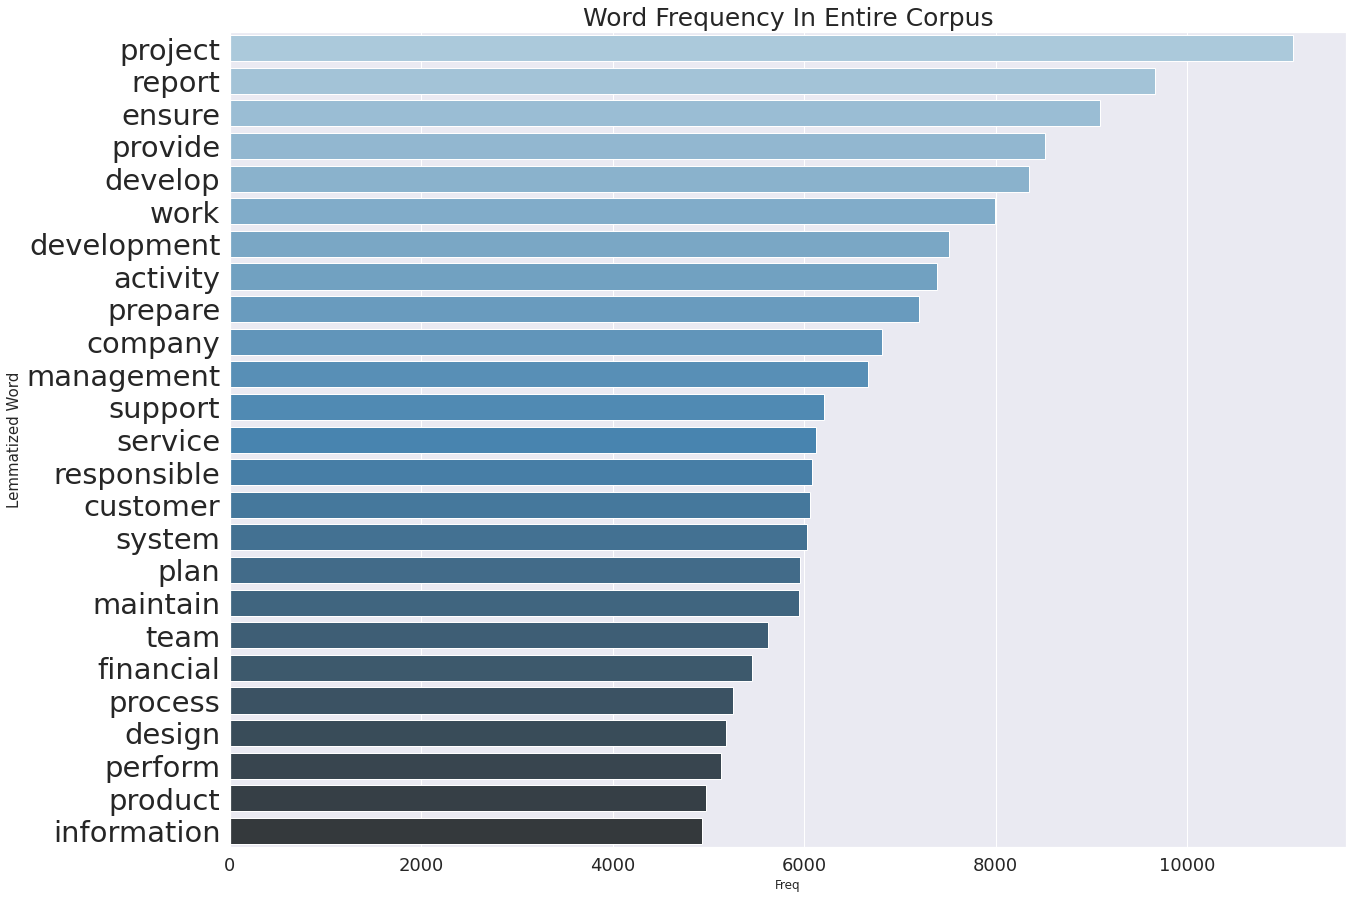
\includegraphics[scale=0.15]{images/frequent_hist.png}
        \caption{ Word Frequency Histogram}
        \label{fig:23}
    \end{minipage}%
    \begin{minipage}[t]{0.5\linewidth}
        \centering
        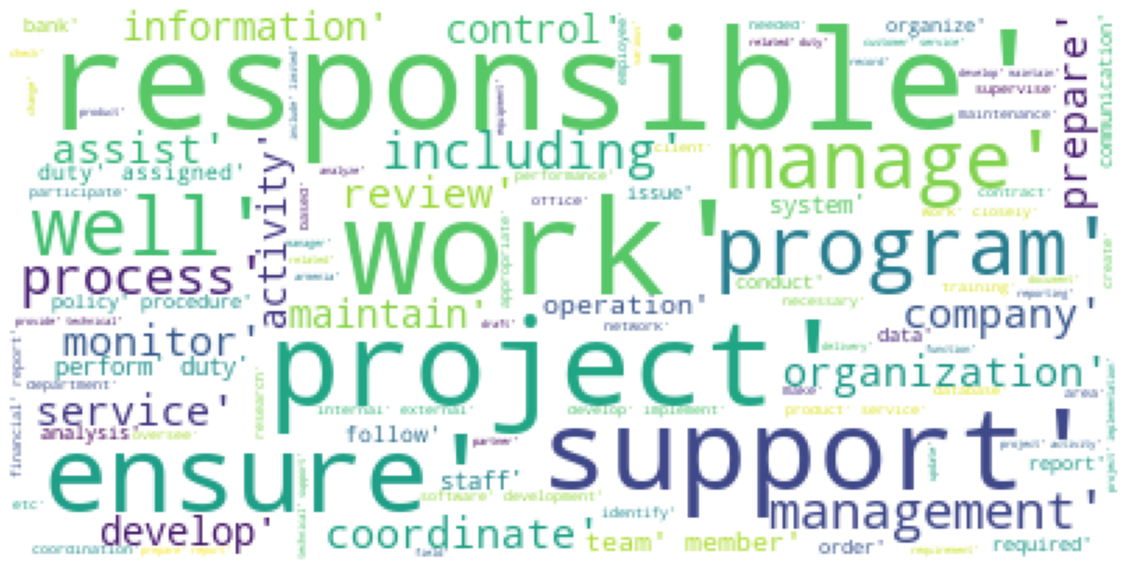
\includegraphics[scale=0.15]{images/frequent_cloud.png}
        \caption{Word Cloud}
        \label{fig:24}
    \end{minipage}
\end{figure}

According to the above figures, it seems that these top single words are indeed close to job positions but not totally skill-related. The most frequent n-grams (including Bigram and Trigram) are demonstrated as follows, which are more likely to be regarded as skill expressions than just single words. 

\begin{figure}[H]
    \begin{minipage}[t]{0.5\linewidth}
        \centering
        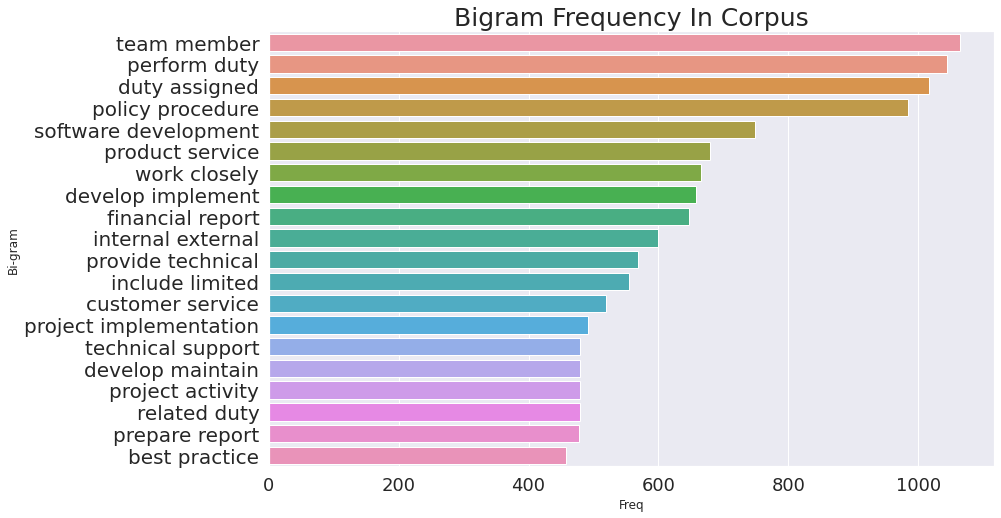
\includegraphics[scale=0.2]{images/bigram.png}
        \caption{Bigram Frequency}
        \label{fig:25}
    \end{minipage}%
    \begin{minipage}[t]{0.5\linewidth}
        \centering
        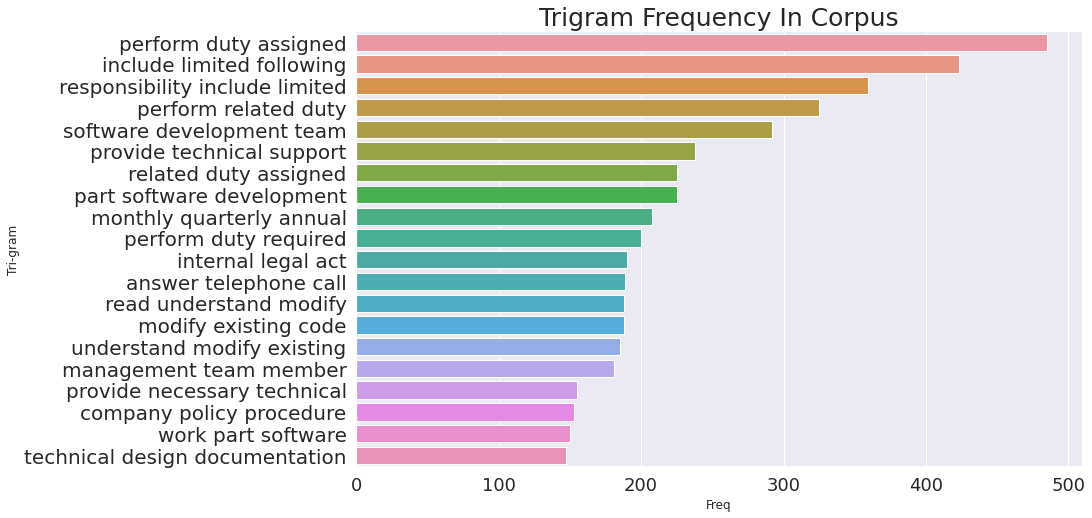
\includegraphics[scale=0.2]{images/trigram.png}
        \caption{Trigram Frequency}
        \label{fig:26}
    \end{minipage}
\end{figure}

% To gain the potential words and phrases for skills, POS tagging is used to get the chunks.


 \begin{figure}[H]
    \centering
    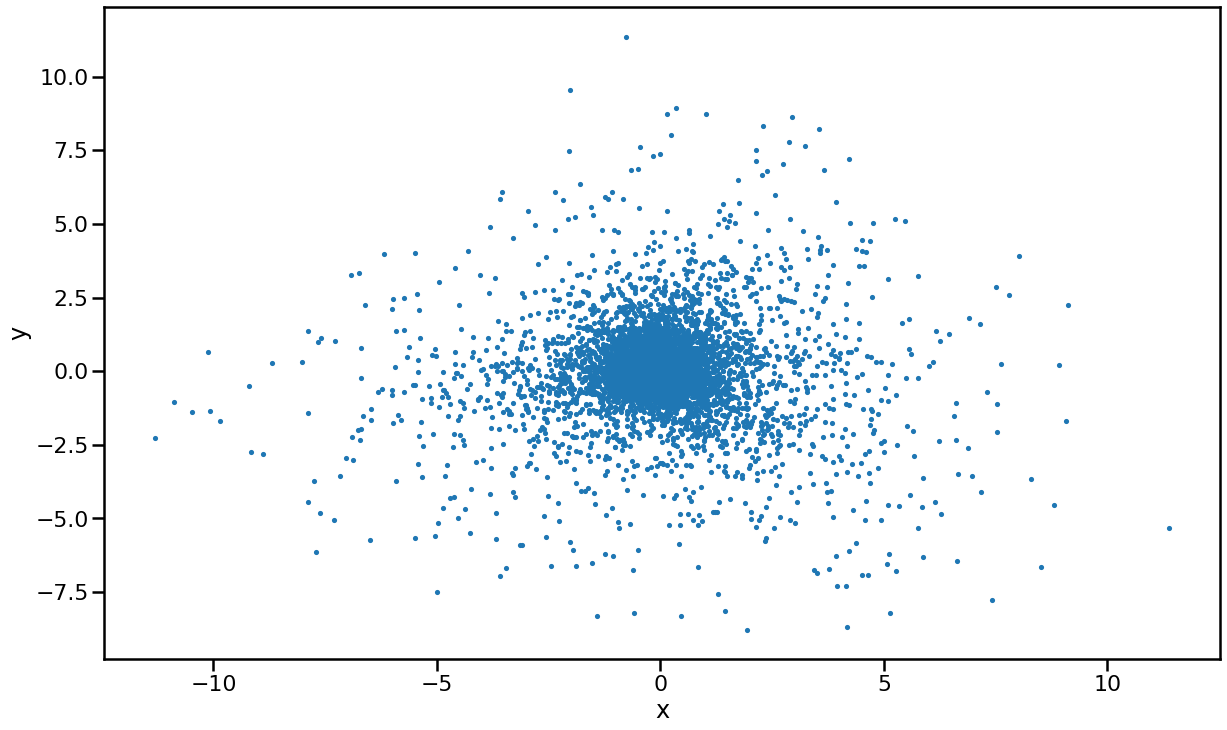
\includegraphics[width=1.0\textwidth]{images/word2vec_scatter.png}
    \caption{Scatter}
    \label{fig:27}
\end{figure}

\subsection{Skill Extraction Result}

\subsubsection{K-means Clustering}

The idea for using K-means algorithm to predict skills in the text is to get K clusters and expect some of the clusters to contain skills. As introduced in Section \ref{sec:word2vec}, word2vec is used to generate the word vectors for clustering. Based on Word2Vec model from Gensim and the pre-trained dataset  GoogleNews-vectors-negative300.bin.gz, which can be downloaded from \href{https://www.kaggle.com/datasets/leadbest/googlenewsvectorsnegative300}{kaggle}, we trained our word2vec model by the preprocessed job description dataset.

The dimension of the word vectors is set to 300; thus, to visualize the result of word2vec, Principle Components Analysis (PCA) is utilized to implement the dimensionality reduction from 300d to 2d. The scatter diagram of the word vectors is shown in Figure \ref{fig:27}, and a piece of the region of the vector points with the corresponding words is shown in Figure \ref{fig:28}.



\begin{figure}[H]
    \centering
    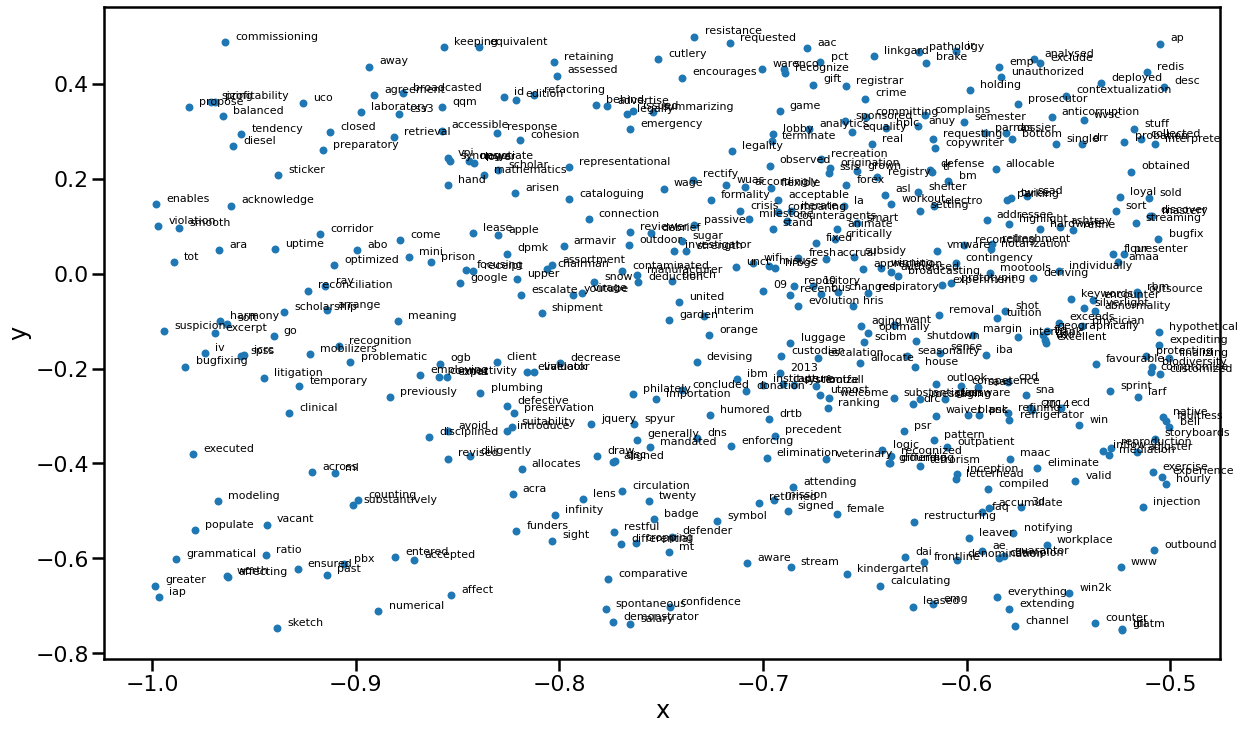
\includegraphics[width=1.0\textwidth]{images/word2vec_words.png}
    \caption{Scatter with Words}
    \label{fig:28}
\end{figure}

With the generated word vectors, the similarity between words can be calculated via 'similar\_by\_word' in Word2Vec module from Gensim. The following figures are screenshots demonstrating two examples, where the input word is the test word and the result presents the top 5 words most similar to the input word with their similarity. Through manual check, the related words computed by word vectors are reasonable, which means the word2vec model performs well.


\begin{figure}[H]
    \begin{minipage}[t]{0.5\linewidth}
        \centering
        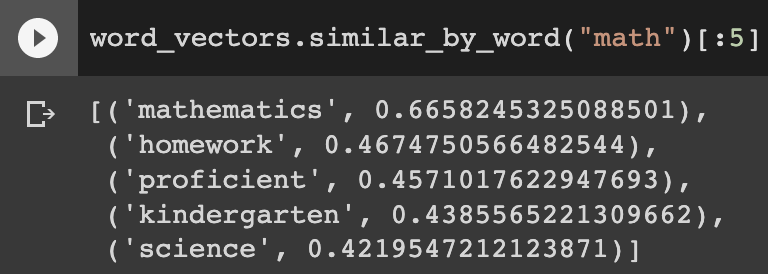
\includegraphics[scale=0.5]{images/wv_exp1.png}
        % \caption{Bigram Frequency}
        \label{fig:29}
    \end{minipage}%
    \begin{minipage}[t]{0.5\linewidth}
        \centering
        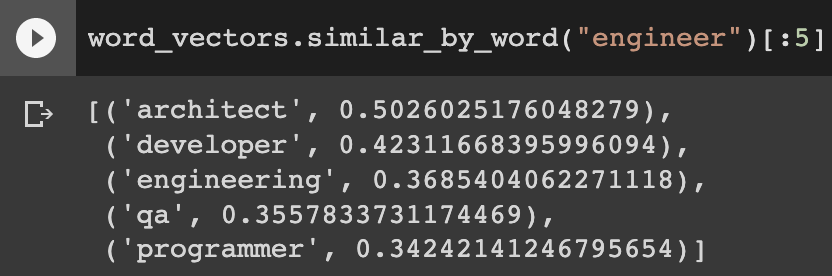
\includegraphics[scale=0.5]{images/wv_exp3.png}
        % \caption{Trigram Frequency}
        \label{fig:30}
    \end{minipage}
    \caption{Examples of Word Similarity}
\end{figure}

By using the word vectors as the training samples, K-menas algorithm could be applied to get clusters. Setting $n\_clusters$ to 12, top members, the 8 most close words of each clustering center, are listed in the following table \ref{tbl:2}. According to the result, some of the clusters are interpretable, where cluster $\#03$ is related to the information of bank or financial position, cluster $\#08$ might be about the verbs appeared in the job description and cluster $\#12$ could be connected to problem solving. But there is no cluster that obvious relate to skill as expected. The reason could be that the skill-related words are not all with the similar meanings, which means that the representation of those words would not be close to each other and would not be gathered in the same cluster. It is a common difficulty for clustering algorithm to deal with this kind of problem. The samples most close to the cluster center are regarded as the top words in K-means algorithm, but they are not the most representative and interpretable samples for the cluster in human-understanding. Moreover, K-means algorithm defines the members of the cluster based on Euclidean distance, and Euclidean distance could not work well in high dimensional data. Additionally, K-means can only detect spherical clusters, which might not fit this text dataset. Consequently, K-means clustering is not a suitable choice for the skill extraction task.


% \begin{figure}[H]
%     \centering
%     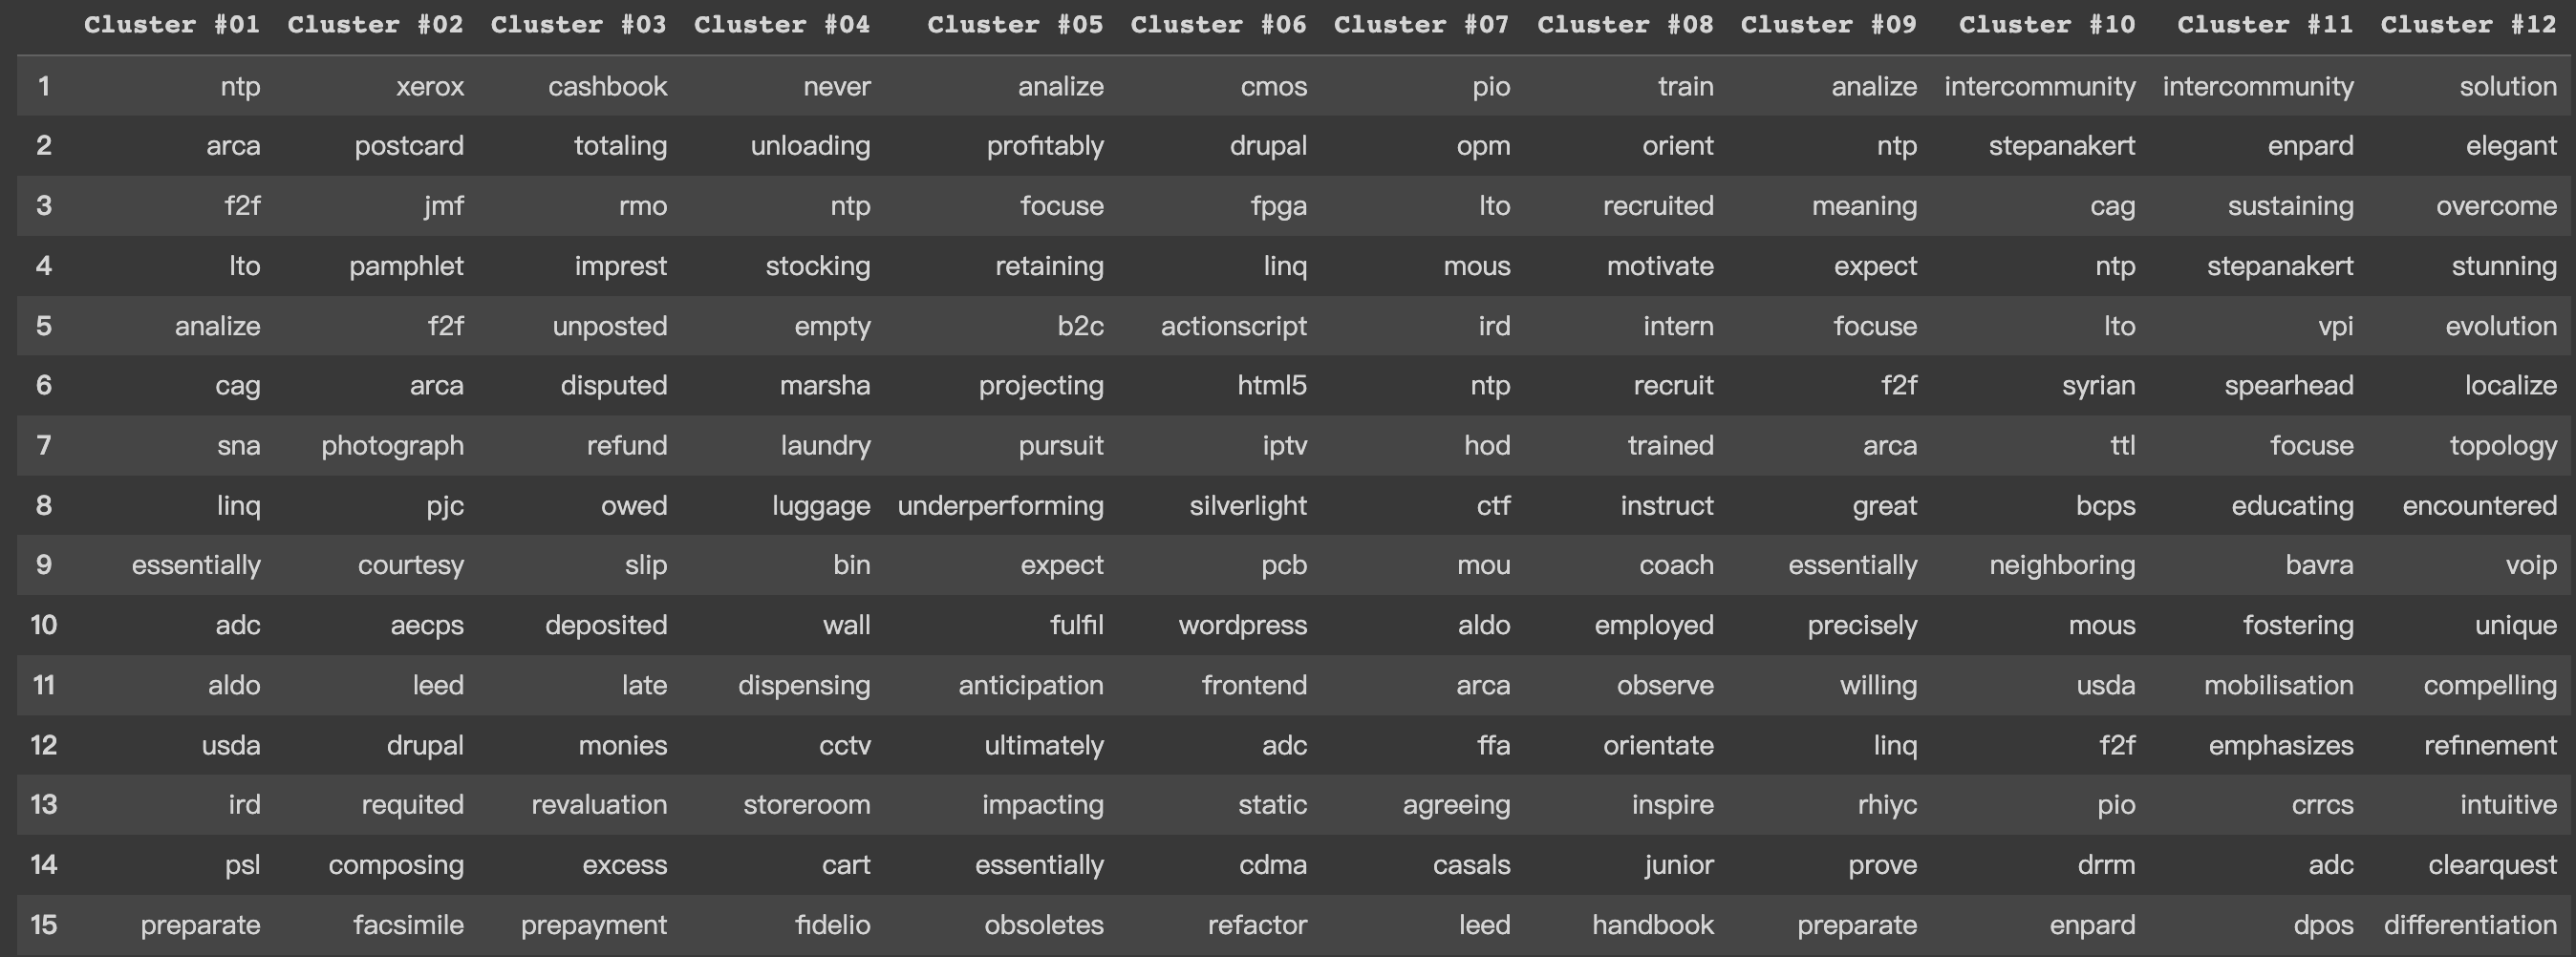
\includegraphics[width=1.0\textwidth]{images/kmeans_cluster.png}
%     \caption{K-means Clusters}
%     \label{fig:31}
% \end{figure}

\begin{table}[htbp]
\centering
\begin{tabular}{|c|c|}
\hline
Cluster ID & Top words\\
\hline
\#1 & ntp arca f2f lto analize cag sna linq\\
\hline
\#2 & xerox postcard jmf pamphlet f2f arca phtograph pjc\\
\hline
\#3 & cashbook totaling rmo imprest unposted disputed refund owed\\
\hline
\#4 & never unloading ntp stocking empty marsha laundry luggage\\
\hline
\#5 & analize profitably focuse retaining b2c projecting pursuit underperforming\\
\hline
\#6 & cmos drupal fpga linq actionscript html5 iptv silverlight\\
\hline
\#7 & plo opm lto mous ird ntp hod ctf\\
\hline
\#8 & train orient recruited motivate intern recruit trianed instruct \\
\hline
\#9 & analize ntp meaning expect focuse f2f arca great \\
\hline
\#10 & intercommunity stepanakert cag ntp lto syrian ttl bcps \\
\hline
\#11 & intercommunity enpard sustaining stepanakert vpi spearhead focuse educating \\
\hline
\#12 & solution elegant overcome stunning evolution localize topology encountered \\
\hline
\end{tabular}
\caption{K-menas Clusters}
\label{tbl:2}
\end{table}

\subsubsection{Topic Modeling}

Similar to the idea of K-means algorithm, topic modeling technique is also utilized to cluster the words in the corpus. The traditional topic model LDA models topics in each document and models words in each topic, which can make the cluster more meaningful and interpretable than K-means. A web application \href{https://palmetto.demos.dice-research.org}{Palmetto} is adopted to evaluate the coherence of obtained top words in each topic. With the input topic top words and a coherence measure selection, Palmetto service will calculate the different types of coherence and return the result. We chose $C_A$ to evaluate the topics, which computes the coherence based on word pairs, a context window, normalized pointwise mutual information (NPMI) and cosine similarity. The top words in each cluster generated by LDA with $topic\_number = 8$ and the coherence score are shown in the following Table \ref{tbl:3}. A few topics seem to be interpretable, and the top words from the LDA model represent the topic(cluster) more precisely than the central words from each centre of K-means model. Topic $\#2$ might be related to the descriptive words for market area and topic $\#5$ is like IT direction. However, the general coherence scores are low and still could not tell a cluster that points to skills. The result is not as expected since the unsupervised clustering algorithm generated the cluster most based on the meaning of the words instead of the category. Moreover, LDA can only model single words while many skill expressions appear as phrases. Therefore, LDA topic model is also not a good choice for this task, and the hybrid approach will be more appropriate.

\begin{table}[htbp]
\centering
\begin{tabular}{|c|c|c|}
\hline
Topic ID & Top words & $C_A$\\
\hline
\#1 & \tabincell{l}{responsible client report data \\develop new service test} & 0.17\\
\hline
\#2 & \tabincell{l}{product strategy manage market \\activity plan develop marketing} & 0.14 \\
\hline
\#3 & \tabincell{l}{information document make administrative \\perform duty provide staff} & 0.12\\
\hline
\#4 & \tabincell{l}{armenian material draft report \\project prepare assist provide} & 0.18\\
\hline
\#5 & \tabincell{l}{support employee database software \\procedure ensure equipment maintain} & 0.15 \\
\hline
\#6 & \tabincell{l}{plan staff training support development\\ implementation activity ensure} & 0.18\\
\hline
\#7 & \tabincell{l}{requirement develop application technical \\software project work development} & 0.28\\
\hline
\#8 & \tabincell{l}{procedure management credit ensure \\control accounting bank prepare} & 0.14\\
\hline
\end{tabular}
\caption{LDA Topics(Clusters)}
\label{tbl:3}
\end{table}


\subsubsection{Hybrid Approach}
\label{sec:bert}

Reviewing the details of the hybrid approach to extract skills in the job description, the main processes after preprocessing are: 1)POS tagging, 2) chunking by regular expressions to get potential skill expressions, 3)labeling the chunks to generate training data, 4)training Neural Network with BERT layer to binary classification.

Experimenting with chunking the data with the four regular expression patterns proposed by \cite{ketterer2}, the obtained chunks contain many unreasonable phrases such as meaningless nouns combination and long phrases with over five tokens, which are not as expected. We find out that in the originally proposed approach, they chunked the tokens directly without doing stop words removal and lemmatization for their dataset. In our implementation, the basic preprocessing steps were applied to our dataset to get a clearer result. Because of removing the stop words such as prepositions and pronouns, nouns and verbs were the main components of the dataset. In this case, the regular expression such as $\{<NN|NNS|NNP>+\}$ would not make sense anymore since there were many consecutive nouns in the dataset, but they should be separated into different chunks. Based on the observation during the experiment, the chunking rules are modified and the two patterns are used to extract the potential skill expressions, where we use constrained numbers to avoid long meaningless noun phrases:

\begin{enumerate}
    \item Noun Phrase: $\{<JJ>*<NN|NNS|NNP>\{1,3\}\}$
    
    \item Verb Phrase: $\{<VBG|VBZ|VBP|VBD|VB|VBN><JJ>*<NNS|NN>\{0,3\}\}$
\end{enumerate}

Over 50,000 chunks are generated in two pickle files with a ratio of 7:3 (Noun Phrase to Verb Phrase) by utilizing the above two regular expression patterns. Since the phrases need to be labeled manually, the sample size should be reduced as much as possible. In order to ensure the samples can represent the characteristics of the original data, the appropriate number of samples is drawn out from each pickle file based on the size ratio of the files. $DataFrame.sample()$ is applied to sample the data randomly. Eventually, around 2,500 phrases are sampled from the pickle files and combined with a text file which contains over 1,500 skills to enrich the training set. The final training data contains over 4,000 phrases, and after labeling, the balance of the training set is shown as the following Figure \ref{fig:32}. 

 \begin{figure}[H]
    \centering
    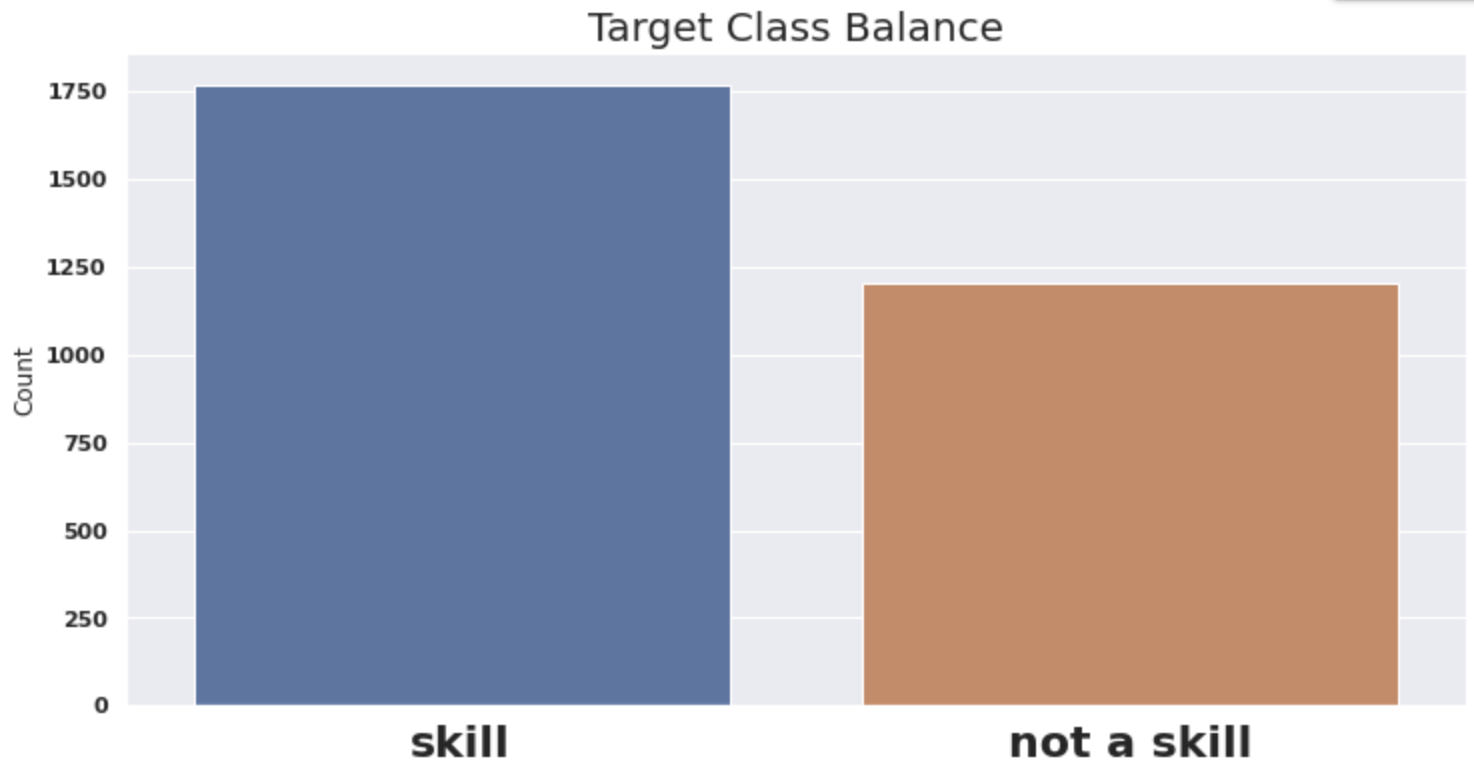
\includegraphics[width=0.8\textwidth]{images/training_set_balance.png}
    \caption{Training Set}
    \label{fig:32}
\end{figure}

Completing building the training dataset, the deep learning neural network with BERT layer is trained to classify the phrases to skill or not skill. The model is built based on Keras in Tensorflow, and the description of layers in the network is as follows:

 \begin{figure}[H]
    \centering
    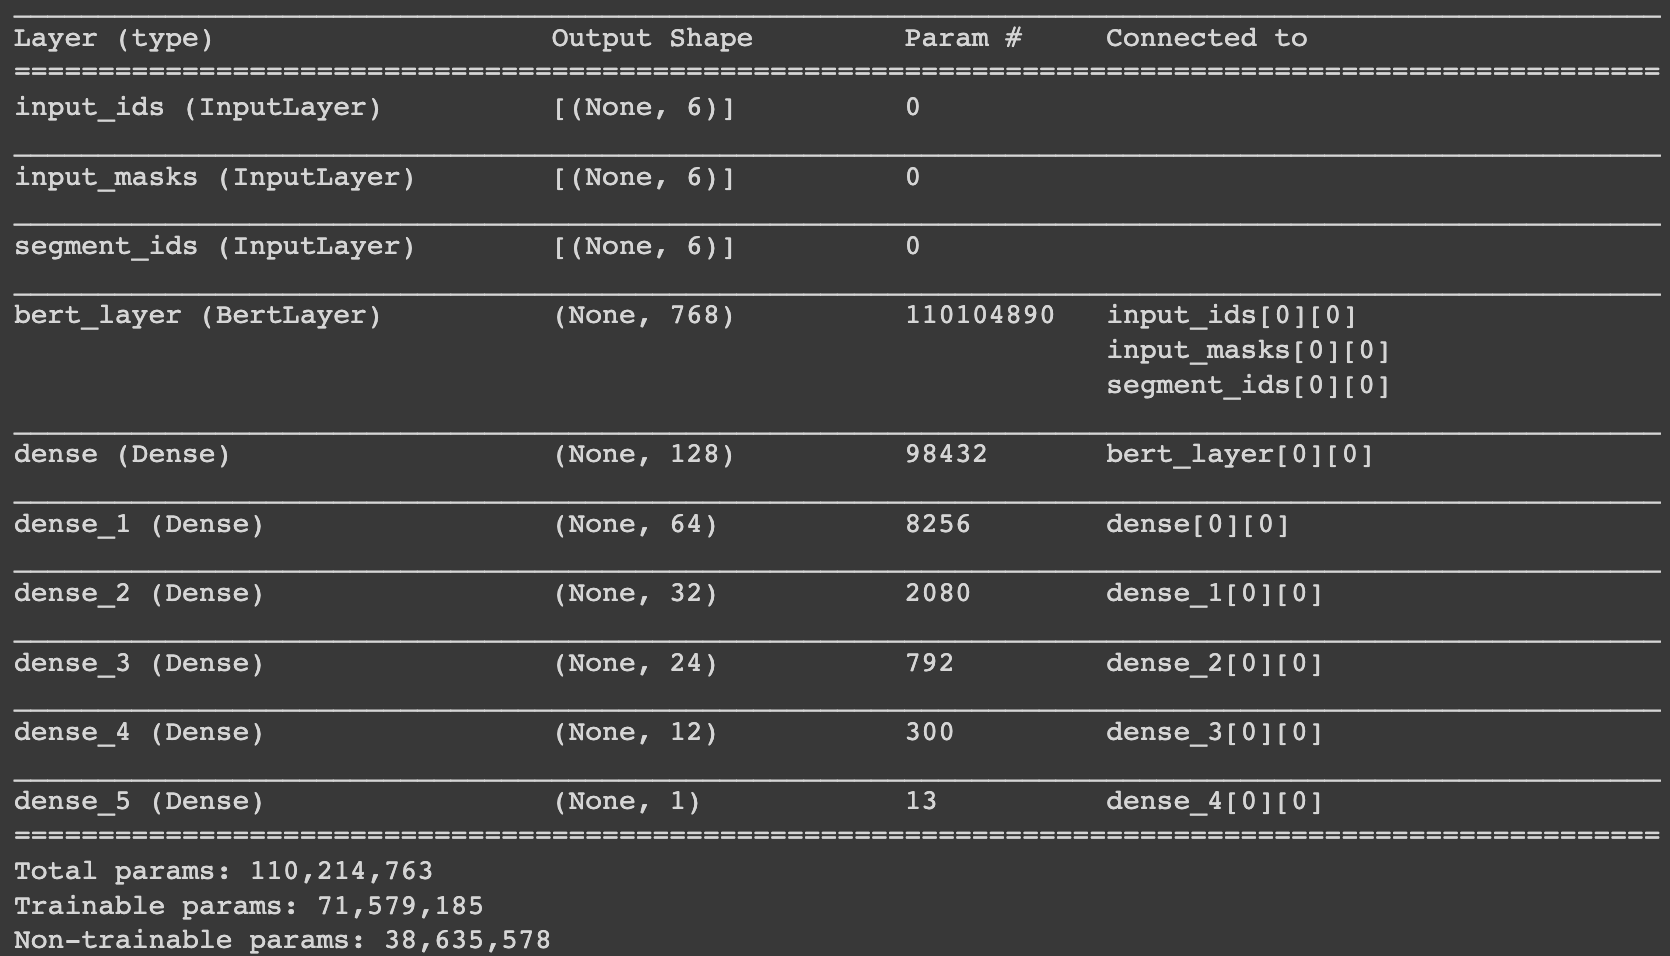
\includegraphics[width=1.0\textwidth]{images/layers_bert.png}
    \caption{Layers of the Classification Model}
    \label{fig:33}
\end{figure}

Splitting the dataset into training and validation data by the proportion of 0.8, the total loss and the accuracy results for both the training set and validation set during training in each epoch are demonstrated in the following figures.

\begin{figure}[H]
    \begin{minipage}[t]{0.5\linewidth}
        \centering
        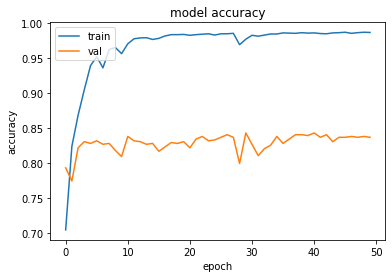
\includegraphics[scale=0.5]{images/acc_graph.png}
        % \caption{Bigram Frequency}
    \end{minipage}%
    \begin{minipage}[t]{0.5\linewidth}
        \centering
        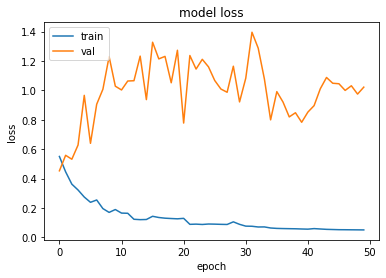
\includegraphics[scale=0.5]{images/loss_graph.png}
        % \caption{Trigram Frequency}
    \end{minipage}
    \label{fig:34}
    \caption{Accuracy \& Loss of the Classification Model}
\end{figure}


% \begin{table}[htbp]
% \centering
% \begin{tabular}{|c|c|c|c|c|}
% \hline
% Epoch & Train\_acc & Val\_acc & Train\_loss & Val\_loss\\
% \hline
% 5 & 0.95 & 0.83 & 0.16 & 0.62\\
% \hline
% 10 & 0.97 & 0.83 & 0.14 & 1.23\\
% \hline
% 15 & 0.98 & 0.83 & 0.04 & 0.91\\
% \hline
% 20 & 0.98 & 0.84 & 0.06 & 0.89\\
% \hline
% 30 & 0.99 & 0.82 & 0.05 & 1.11\\
% \hline
% \end{tabular}
% \caption{Result of Classification Model}
% \label{tbl:5}
% \end{table}

According to Figure \ref{fig:34}, the loss of validation data during 50 epochs is unstable and has a trend towards increasing, though the accuracy and loss of the training set continuously decline, which means the model might encounter the overfitting problem. To balance the total loss and the accuracy of both the train and validation data, the number of epochs is set to 20. Then, the BERT model got an accuracy of 0.98 with the training data, and 0.84 with the validation data.

In addition, another piece of job posting text from the Internet was tested as unseen data. After preprocessing and chunking the text, the extracted phrases from the data are manually labeled to get the prediction result. Dealing with this unseen data, our model got an accuracy of 0.75 and a loss of 3.88. The accuracy of the model on the testing data is acceptable. However, some phrases are not very interpretable, which will be discussed in Section \ref{sec:visual} with the visualization result. 




\subsection{Matching Result}

The original idea of matching the resume to the position is to match their skills on the condition that most skills are extracted. But as mentioned in Section \ref{sec:ner_result}, the performance of the NER model on recognizing skills in the resume was not as expected. Several real-world resumes were tested but few skills were extracted successfully. Therefore, we decided to use cosine similarity between the whole resume text and the job description to get the final match rate. The result is hard to be quantitatively evaluated since there is no standard measure to determine the match rate of two text data. So we compared our result with an existing robust CV checker \href{https://careerset.com/}{CareerSet} via different test cases to check whether our result is reasonable. The following table shows the match rate results from CareerSet and our application.

\begin{table}[htbp]
\centering
\begin{tabular}{|c|c|c|c|}
\hline
Test Case & CareerSet & Our Application\\
\hline
1 & 43\% & 50.42\%\\
\hline
2 & 75\% & 48.34\%\\
\hline
3 & 47\% & 62.1\% \\
\hline
\end{tabular}
\caption{Comparison of Match Rate Result}
\label{tbl:5}
\end{table}

The three test cases used the same resume and targeted to three different kinds of positions. According to the result, for low matching, such as test case 1, the result of our application is close to that from CareerSet. For case 2, the resume and the target position should have a high match, while our application generated a low match result. It is a limitation of regarding the cosine similarity of entire contents as the match rate between the resume and the target position. Because resume and job description data have totally different styles, the high match rate does not need the high similarity of the contents. 


\section{Overall Evaluation}
\label{sec:visual}



Based on the techniques for content checking and skill extraction, the visualization result of the application is shown in the following Figure \ref{fig:36}. The match rate from the resume to the job description is presented at the top of the page. As for the resume content check, according to the figure, the checklist contains Name, Email address, College, Degree, Designation and Skills. When recognizing the entities in the resume, the content of the named entity will be shown in the table. If the entity on the checklist has not been detected, the content column will print 'Not Detected' instead. The input resume contains all named entities on the checklist, but the email address and skills are not detected by our application, which is caused by the performance of the NER model. 

The extracted skills from the job description are listed at the bottom of the page. As illustrated in Section \ref{sec:bert}, though the deep learning model with BERT layer got high accuracy, the chunks predicted to be skills are not entirely reasonable and interpretable. According to the extracted skills listed in the figure, some irrelevant nouns were chunked together based on the regex patterns, and some chunks contained more than one skill. Setting more different regex for chunking might get a better result, but since the representation of skills is various, it is hard to define the most suitable regex chunking patterns. It can be regarded as the limitation of the regex-based chunking algorithm to extract phrases. Moreover, some phrases were not skill-related but were classified as skill, while some skills were predicted to be non-skill, which might be caused by the performance of the BERT model. The neural network training set needs to contain more job position fields to cover more skills in different areas. Furthermore, since the training data was labeled manually, labeling mistakes could not be eliminated, which would also affect the prediction result.


% 1. (limitation) chunks might got wrong, combinition of several skills
% 2. training set does not contain enough field of job
% 3. more or different regex might be found for better result
% 4. BERT NN part is fine
% 5. manual labeling with mistakes

 \begin{figure}[H]
    \centering
    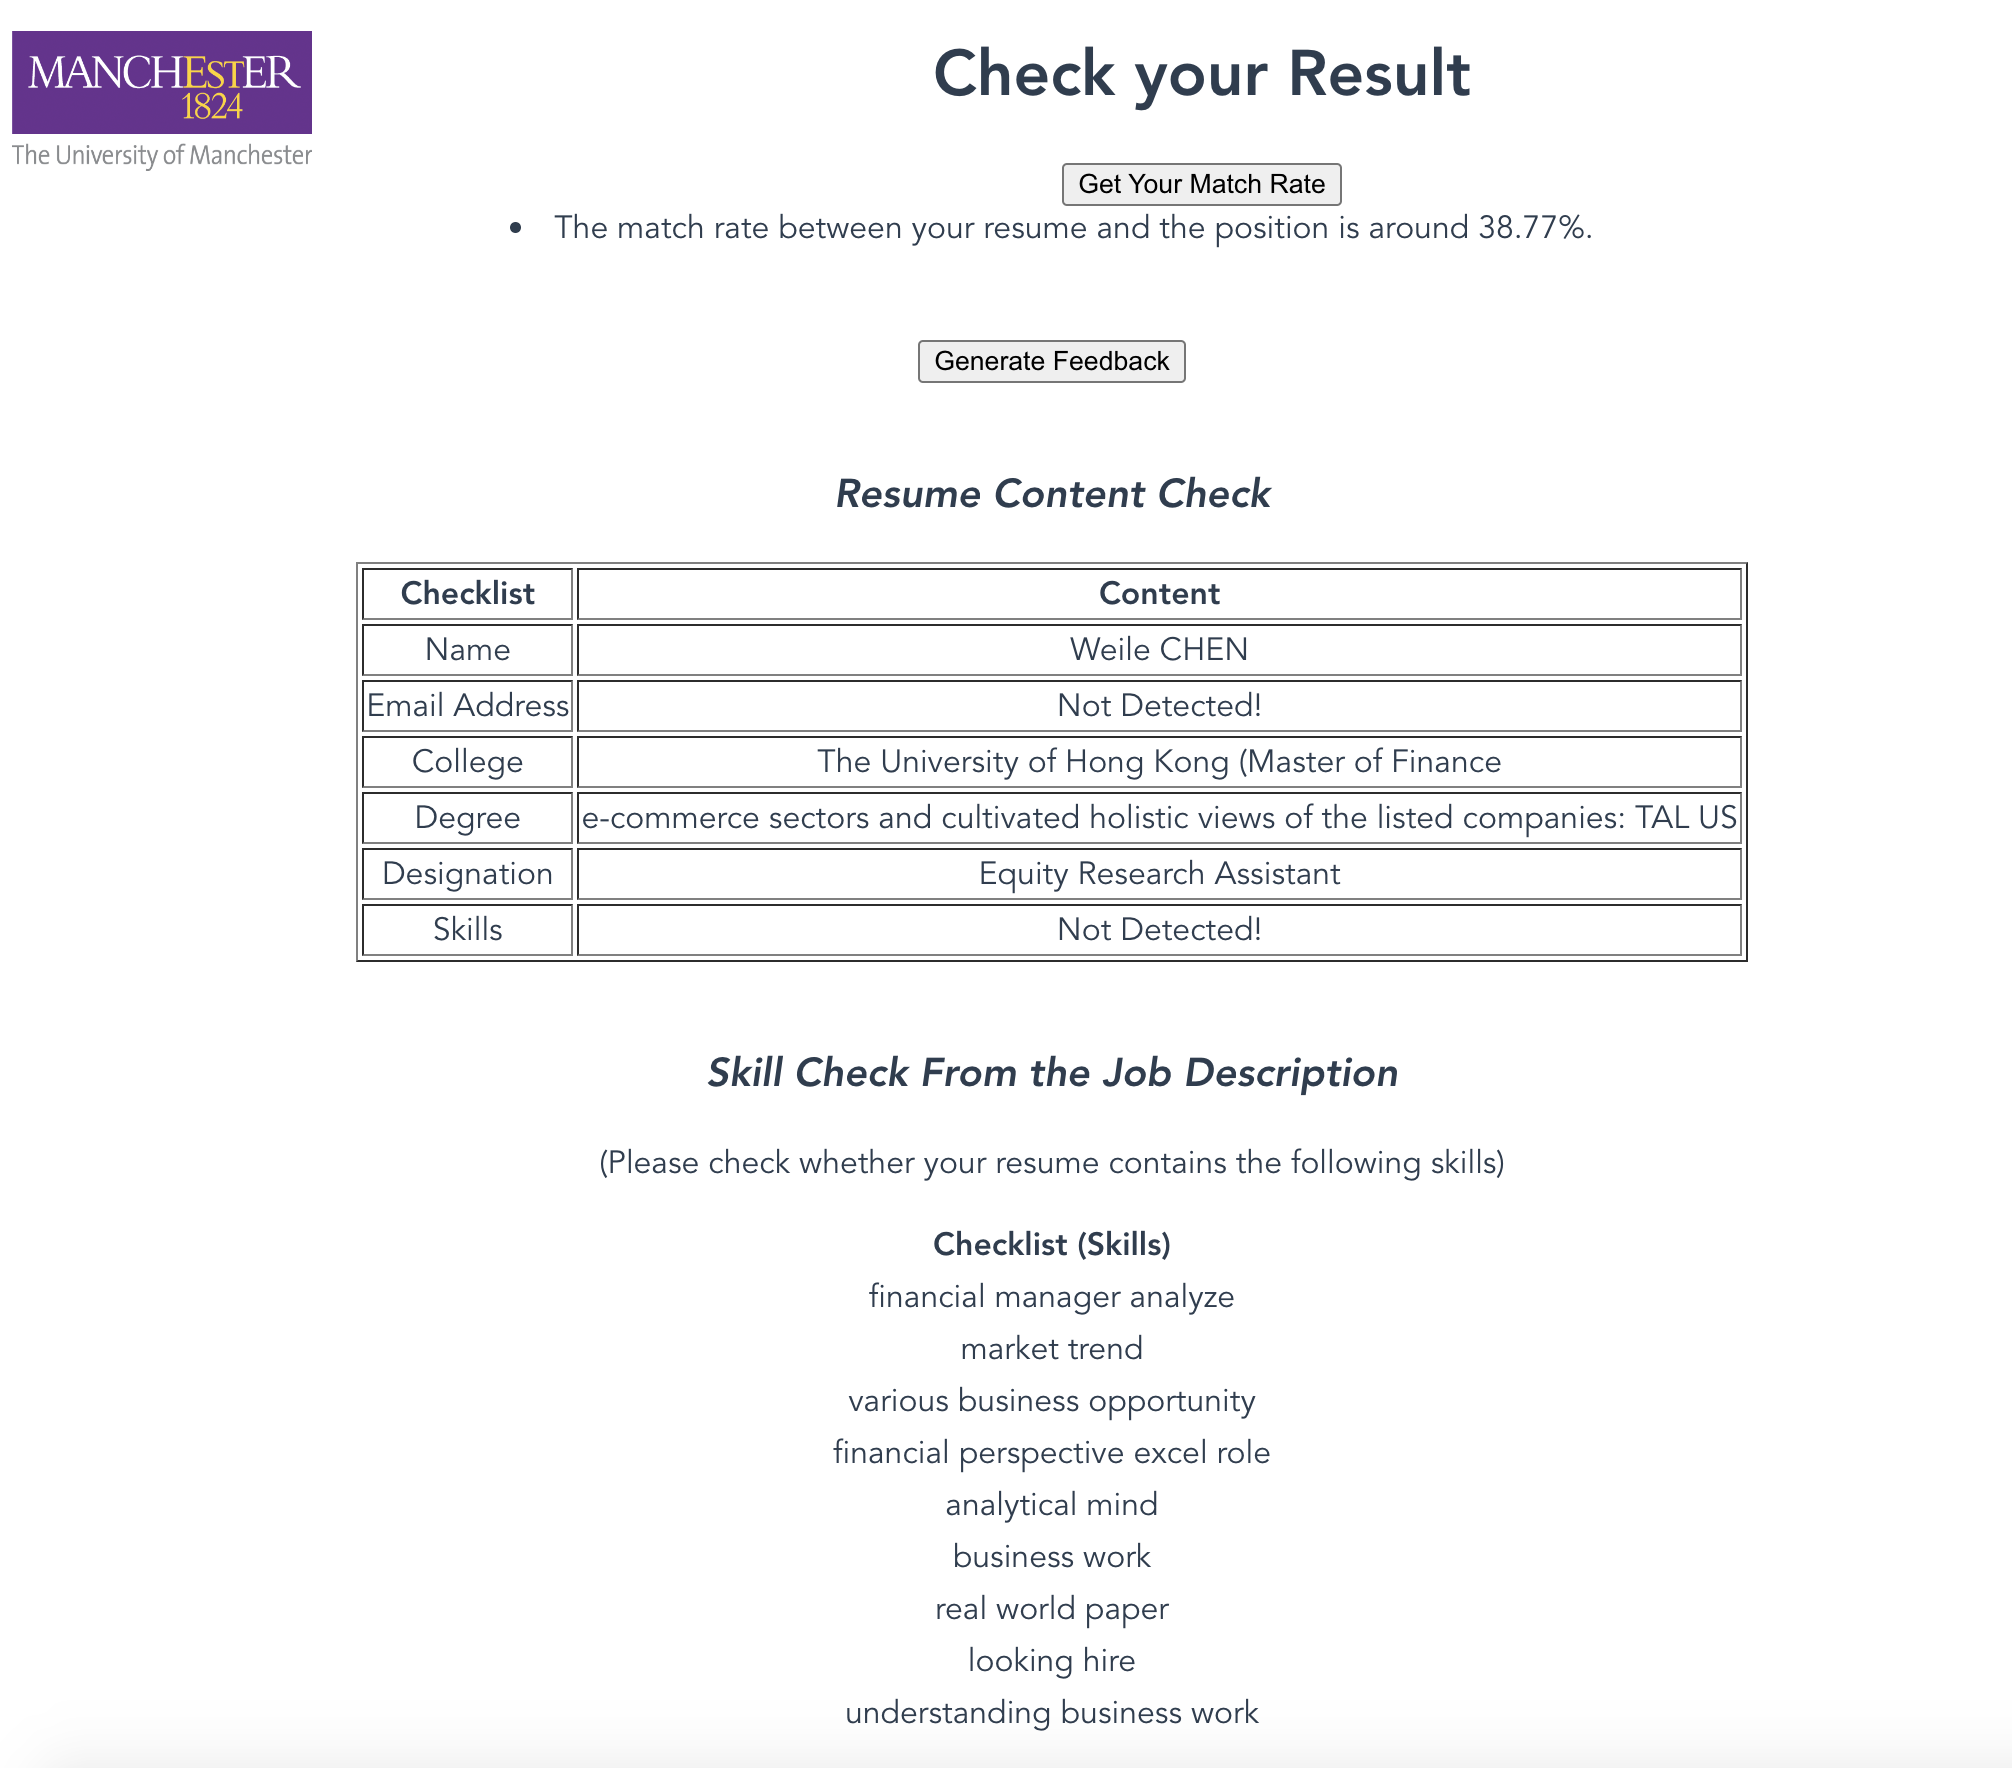
\includegraphics[width=1.1\textwidth]{images/visual.png}
    \caption{Screenshot of the Feedback Page}
    \label{fig:36}
\end{figure}

\chapter{Conclusion}
\label{ch:conclusion}
This chapter will summarize the project by concluding the achievements, discussing the reflections and limitations, and identifying the future work of the project. 


\section{Achievements \& Contribution}

In this project, we developed a web application for CV checking based on NLP techniques and Machine Learning algorithms. The main achievements can be divided into two parts, one is researching and implementing different techniques to achieve some of the functionalities in the existing CV checker, and the other is developing our own CV checker by applying those techniques. More specifically, the research and experimentation were mainly focused on the task of resume parsing, information identification, skill extraction and skill matching.

Firstly, we collected the resume and job description dataset, and chose suitable preprocessing techniques to prepare the data. Subsequently, to meet the requirements, we had in-depth research and experiments on the related techniques and systems of the target tasks. Based on an annotated resume dataset, we trained an NER model to recognize important named entities in the resume with a precision of over 0.95 in some kinds of named entities. As for the skill extraction task, we implemented K-means clustering, LDA topic model and a hybrid approach proposed by Ketterer \cite{ketterer}. After comparing the results, the hybrid approach was chosen for recognizing skills. In order to fit our dataset, we did modifications and improvements from the initially proposed algorithm, and got acceptable performance with an accuracy of over 0.8. Furthermore, applying the trained models, a web application was developed. The CV checker allows user to upload their CV and job description, then returns the feedback of the resume on both content check and the match details between the resume and the position. Despite the current limitations of the deliverable, this application met the basic requirements. 



\section{Reflection}

Through reviewing the entire experiments and development process, there are some limitations, and the project still has room for improvement. Firstly, as discussed in Section \ref{sec:match}, the match rate between the resume and the job description by computing the cosine similarity of the two texts is not robust. Matching the resume and job description keywords might get a more reasonable result. 

As mentioned in \ref{sec:ner_result}, though the NER model for information identification performed well in recognizing many named entities, the recognition ability was still weak. When testing new resumes which are not in the train and validation set, some important information was missing, and few recognized entities were not exactly correct. The insufficient and imbalanced training set for the NER model could be one effect of the recognition result. The patterns' similarity within a named entity could also influence the performance, where the performance might get worse if there are various patterns for one entity in different resumes. Moreover, to eliminate the entity-overlapping problem, we had to remove some annotations in the training set, which also affected the model performance.

There are some limitations on the implementation of the skill extraction task as well. Without a massive and reliable skill database, we utilized basic NLP techniques and a deep learning model to identify the skills in job description text with the idea from Ketterer \cite{ketterer}. The performance of the neural network to binary classify the phrases was acceptable, but the latent skill-related phrases extracted by regex chunking were not that satisfied. Using regular expression to obtain the potential skill chunks based on POS tags could identify some skill phrases, but might also get uninterpretable expressions; for instance, part of the phrase is skill while the rest is not related. Therefore, the skill extraction result is extremely reliant on the setting of the regex. But it is a hard task to define commonly used regular expressions of skills since the representation of skills is various. 

As for the application, the functionalities are limited. The current deliverable can get the matching result between the resume and the position, and can check the basic content of the resume, such as name, e-mail address, college name and degree. According to the existing powerful CV checkers, word use, writing style, and format also matter in the resume and need to be checked, which can be regarded as future work for our project. Additionally, the current parser could only parse the resume written in one column, which is also a limitation.

\section{Future Work}

According to the limitations pointed out in the previous section, improvements could be made in several aspects of this project. The first issue that needs to be focused on is refining the dataset. It is vital to extend the training set with consistency named entity labels to identify the important information in the resume more accurate and efficient with the NER model. In addition, a Bi-LSTM-CRF model for sequence labeling proposed by Huang et al. \cite{huang2015bidirectional} is said to be robust and result in state of art accuracy on the NER dataset, which can be referred to improve our NER model. 

As for the skill extraction task, our hybrid approach with BERT model can be enhanced by setting more specific regex and obtaining more interpretable chunks. Smith et al. \cite{smith2021skill} proposed a syntactic approach for word embedding enabling to model a significant distinction between skill terms and non-skill terms, which can be combined with our model. Generally, identifying skills in job description data is a complex and study-worthy research question. In order to get a precise result of extracting skills, more effort is needed for research and experimentation in the future. According to an existing skill extractor \href{https://github.com/AnasAito/SkillNER}{SkillNER}\cite{skillner}, rule-based NLP module can get excellent performance if there is a reliable and massive skill database. Therefore, our subsequent research should not be restricted to improving the output result of the machine learning model since building a dependable skill database might get a more efficient result. Furthermore, defining the soft skill and hard skill from the extracted skills should also be taken into consideration for further development. 

With regard to the usability of the application, there are many other functionalities can be implemented to get a more powerful CV checker in the future. Firstly, since this project put emphasis on the back-end algorithms, the user interface of the application is currently quite simple. Further development can be on optimizing the UI and the visualization result. Subsequently, checking word use, format, spelling and writing style could all be taken as the inspiration for further development. Additionally, a resume ranking system for companies to screen the candidates for a position is proposed by Amin et al \cite{amin2019web}. It can be defined as the future developing direction of our project, that extends the target users from only job seekers to both job seekers and recruiters by accepting multiple resumes as input and returning the ranking of them.


% skill extraction is a complex work, need reliable and huge dataset to get better result

% extend training data

% read different style of resume (e.g. two columns)

% for functionality of CV checker

% each part of the back-end algorithms

%\include{chapter_a}
%\include{chapter_b}
%\include{chapter_c}

\bibliography{refs}    % this causes the references to be listed

\bibliographystyle{plain}
% \bibliographystyle{abbrv}
% \bibliographystyle{apacite}
%% the bibliography style determines the format  in which both citations and references are printed,
%% other possible values are plain and abbrv
%%
%% If you want more control of the format of your citations you might want to take a look at
%% natbib.sty, which should be part of any standard LaTeX installation
%%
%% University regulations simply require that your citation style be consistent, so see what style
%% your supervisor recommends.

% Appendices start here

\appendix
% \chapter{Image Compositions in Blender}
\label{cha:appendix1}

% \chapter{Code Snippets of Wasserstein Loss with Gradient Penalty}
\label{cha:appendix2}


\end{document}
